% arara: pdflatex
% arara: bibtex
% arara: makeglossaries
% arara: pdflatex
% !arara: pdflatex
% !arara: indent: {overwrite: yes, trace: on}
\documentclass[11pt,twoside]{report}
%= == == == == == == == == == == =
%
% Document details: Program review for the mathematics department
%       at Portland Community College, Portland OR
%
%       Prepared in Fall 2013
%
%= == == == == == == == == == == =
\usepackage[headheight=14pt,left=3.5cm,right=2.0cm,showframe=false,
top=2cm,bottom=1.5cm,asymmetric=true,bindingoffset=1cm]{geometry}               
\usepackage{parskip}
\usepackage{titlesec}                   % customize headings
\usepackage{titletoc}                   % customize tableofcontents
\usepackage{multirow}                   % multirows in tables
\usepackage{booktabs}                   % beautiful tables
\usepackage{flafter}                    % floats won't appear until after they appear in the code
\usepackage[figuresright]{rotating}     % sideways table
\usepackage{longtable}                  % tables that can break across pages
\usepackage{fancyhdr}                   % headers and footers
\usepackage{standalone}                 % maintain graphs and tables in separate files
\usepackage{pdfpages}                   % include separate pdf documents
\usepackage{enumitem}                   % customization of list environments
\usepackage{changepage}                 % adjust margins for selected portions
\usepackage{tablefootnote}              % footnotes within tables
\usepackage[sc,hang]{caption}           % customize captions of tables and figures
\usepackage{subcaption}                 % subfigures and subtables
\usepackage[charter]{mathdesign}        % font choice
\usepackage{microtype}                  % better kerning
\usepackage{siunitx}                    % elegant handling of units
\usepackage{pgfplotstable}              % typeset tables intelligently
\usepackage{tcolorbox}
\usepackage{etoolbox}
\usepackage{epigraph}                   % for inspirational quotes
\usepackage[backend=bibtex,maxnames=99]{biblatex}   % bibliography
\usepackage{varioref}                   % good for referencing things 'far away'
\usepackage{hyperref}                   % hyperlinks
\usepackage{pdfcomment}		% for inserting of tooltips, like with fix this items
\usepackage{bookmark}
\usepackage{cleveref}                   % allows \cref and friends
\usepackage{refcheck}                   % checks if labels have been used remove once the document is completed
%\usepackage[left]{showlabels}
%\showlabels{hypertarget}
%\showlabels{hyperlink}

% tcolorbox libraries
\tcbuselibrary{breakable,skins}

% hyperlink setup
\hypersetup{colorlinks=true,
	linkcolor=blue,
	citecolor=black,
}

% bibliography settings
\addbibresource{pccbib}

% cleveref settings
\crefname{table}{Table}{Tables}
\Crefname{table}{Table}{Tables}
\crefname{figure}{Figure}{Figures}
\Crefname{figure}{Figure}{Figures}
\crefname{chapter}{Section}{Sections}
\Crefname{chapter}{Section}{Sections}
\crefname{section}{Section}{Sections}
\Crefname{section}{Section}{Sections}

% graphics path
\graphicspath{{./graphics/}}

% axis style, ticks, etc
\pgfplotsset{every axis/.append style={
	legend cell align=left,       % otherwise width won't be as intended: http://tex.stackexchange.com/questions/36297/pgfplots-how-can-i-scale-to-text-width
}}

% percentage style for tables
\pgfplotstableset{percentstyle/.style={
	preproc/expr={##1*100},
	dec sep align,fixed,fixed zerofill,
	postproc cell content/.append code={
		\ifx\\##1\\% check if ##1 is empty
		\else
		\ifnum1=\pgfplotstablepartno
		\pgfkeysalso{@cell content/.add={}{\,\%}}%
		\fi
		\fi
	},
	precision=0,
	},
	sectionFTPT/.style={
		every head row/.style={
			before row=,percentstyle},
		columns/above100/.style={column name={Above 100 level},column type=r},
		columns/a100percent/.style={column name={\%},percentstyle},
		columns/totpercent/.style={column name={\%},percentstyle},
		columns/total/.style={column name={Total},column type=r},
	}
}

% for the section counters for each chapter
\newcommand{\numbertotext}[1]{%
	\ifcase#1
	zero%
	\or
	one%
	\or
	two%
	\or
	three%
	\or
	four%
	\or
	five%
	\or
	six%
	\else
	% we don't care about the number of sections in chapters greater than 6
	unimportant
	\fi
}

% empty column type- very useful for big tables that ignore columns
\newcolumntype{H}{>{\setbox0=\hbox\bgroup}c<{\egroup}@{}}

% glossaries settings- load after hyperref: http://tex.stackexchange.com/questions/1863/which-packages-should-be-loaded-after-hyperref-instead-of-before
\usepackage[nonumberlist,section=chapter,toc]{glossaries}
% make the links black
\renewcommand*{\glstextformat}[1]{\textcolor{black}{#1}} 
% basic vocab
\newglossaryentry{ADA}{name=ADA,description={Americans with Disabilities Act}}
\newglossaryentry{ALC}{name=ALC,description={Alternative Learning Center. The Alternative Learning Center was the previous name given to the current Student Learning Center \fixthis{Alyson wants a better description}}}
\newglossaryentry{ALEKS}{name=ALEKS,description={ {\bfseries A}ssessment and {\bfseries LE}arning in {\bfseries K}nowledge {\bfseries S}paces interactive computer-based math-learning program owned by McGraw-Hill \url{http://www.aleks.com/}}}
\newglossaryentry{AMP}{name=AMP,description={Accelerated Mathematics Program}}
\newglossaryentry{AY}{name=AY,description={Academic Year}} 
\newglossaryentry{CIC}{name=CIC,description={Completion Investment Council}} 
\newglossaryentry{CTE}{name=CTE,description={Career Technical Education}} 
\newglossaryentry{OSD}{name=OSD,description={Office of Students with Disabilities}} 
\newglossaryentry{CCOG}{name=CCOG,description={Course Curriculum and Outcome Guide}} 
\newglossaryentry{DL}{name=DL,description={Distance Learning}} 
\newglossaryentry{DOI}{name=DOI,description={Deans Of Instruction}}
\newglossaryentry{F2F}{name=F2F,description={Face-to-face}} 
\newglossaryentry{FT}{name=FT,description={Full-time (usually in reference to faculty)}} 
\newglossaryentry{LAC}{name=LAC,description={Learning Assessment Council}} 
\newglossaryentry{LAS}{name=LAS,description={Learning Assessment Subcommittee (of the LAC)}} 
\newglossaryentry{LDC}{name=LDC,description={Lower Division Collegiate}} 
\newglossaryentry{MyMathLab}{name=MyMathLab,description={MyMathLab-- a commercial computer-based homework management system owned and distributed by Peason \url{http://www.pearsonmylabandmastering.com/northamerica/mymathlab/}}}
\newglossaryentry{PT}{name=PT,description={Part-time (usually in reference to faculty)}} 
\newglossaryentry{SAC}{name=SAC,description={Subject Area Committee}}
\newglossaryentry{WRC}{name=WRC,description={Women's Resource Center}}
\makeglossaries

% to do:
%   - shorten toc entries where necessary, indentation of toc, generally tidy it
%   - glossary items, and update glossary entries throughout using perl script
%   - add 'colophon' (maybe?): http://tex.stackexchange.com/questions/63468/what-is-best-way-to-mention-that-a-document-has-been-typeset-with-tex
%   - make consistent choice about on-campus, oncampus, on campus, online (online and on-campus are the winners)
%   - make consistent choice about full-time, full time, part-time, part time (full-time and part-time win)
%   - change all 'adjunct' to 'part time' (or 'part-time')
%   - make consistent choice about face 2 face or face-to-face (face-to-face wins, F2F can be used in tables; DL is fine anywhere)
%   - check that all sections in the appendix are referenced in the body 
%       (use refcheck package to check the output and grep the log file)
%   - address all fixthis issues (check output and .log file)
%   - check for undefined references, multiply defined labels- grep log file
%   - give headings to paragraphs when appropriate using \paragraph{}?
%   - do we need the bookmark package? are we getting bookmarks in the sidepane?
%   - check that vref, cref, etc know what to do with references at the subsection level; note: use page references instead
%   - check that no hyphens, em dashes, or en dashes have spaces before or after them (except hanging hyphens)
%   - check that hyphens, em dashes, en dashes are used appropriately
%   - go through log file- a few bibliography entries, too
%   - are we doing titles? e.g Mr, Dr, Ms? should be consistent. Decision from Steve, Alex, Chris: no titles
%   - hyperlink Q1, Q2, etc in chapter 6 to their respective questions in the appendix

% Define fix command
% 	- it puts a comment in the margin
% 	- it writes to a file with a list of things that need fixing
\newcommand{\fixthis}[1]
{%
	\marginpar{\huge \color{red} \pdftooltip{\framebox{FIX}}{#1}}%
	\typeout{FIXTHIS: Section \thechapter:  p\thepage : #1^^J}%
}

% for the section pictures
\makeatletter
\newcommand{\cmh}[2]{%
	% we need the first argument to be a number
	% http://tex.stackexchange.com/questions/50111/how-to-check-if-the-value-of-a-parameter-is-a-number
	\if\relax\detokenize\expandafter{\romannumeral-0#1}\relax
	\@ifundefined{c@totalsections@\numbertotext{#1}}%
	{%
		\newcounter{totalsections@\numbertotext{#1}}
		\setcounter{totalsections@\numbertotext{#1}}{#2}
		\typeout{Defining a new counter: totalsections@\numbertotext{#1}} 
	}%
	{%
		\ifnum\value{totalsections@\numbertotext{#1}}=#2
		\typeout{Total sections for Chapter #1 match auxilary file (#2)}
		\else
		\typeout{Warning: total sections for Chapter #1 updated from \the\value{totalsections@\numbertotext{#1}} to #2-- recompile to fix}  
		\fi
		\setcounter{totalsections@\numbertotext{#1}}{#2}
	}%
	\else
	\fi
}

% custom petal shape
% custom petal shape
% custom petal shape
% http://tex.stackexchange.com/questions/151962/rotating-a-custom-shape-independently-of-the-text/151978?noredirect=1#151978
\pgfkeys{/pgf/shape border rotate/.initial=0}

\pgfdeclareshape{petal}
{
	\inheritsavedanchors[from=circle] % this is nearly a circle
	\inheritanchorborder[from=circle]
	\inheritanchor[from=circle]{center}
	\inheritanchor[from=circle]{base}
	\savedmacro\petalparameters{%
		\pgfmathsetmacro\shapeborderrotate{\pgfkeysvalueof{/pgf/shape border rotate}}%
		\addtosavedmacro\shapeborderrotate%
	}
	\backgroundpath{
		% origin
		\petalparameters%
		{% Make sure transformations are  inside group.
			\pgftransformshift{\centerpoint}%
			\pgftransformrotate{\shapeborderrotate}%
			\pgfutil@tempdima=\radius%
			\pgfpathmoveto{\pgfqpoint{\pgfutil@tempdima}{0pt}}%
			\pgfpatharc{0}{180}{\pgfutil@tempdima}%
			\pgfpathcurveto{\pgfqpoint{-\pgfutil@tempdima}{-.5\pgfutil@tempdima}}%
			{\pgfqpoint{-.5\pgfutil@tempdima}{-.75\pgfutil@tempdima}}%
			{\pgfqpoint{0pt}{-1.5\pgfutil@tempdima}}
			\pgfpathcurveto{\pgfqpoint{0pt}{-.75\pgfutil@tempdima}}%
			{\pgfqpoint{\pgfutil@tempdima}{-.75\pgfutil@tempdima}}%
			{\pgfqpoint{\pgfutil@tempdima}{0pt}}%
		}%
	}
}

% boolean switch to tell if we're in the appendix or not
\newbool{inappendix}

% make epigraph italic
\let\oldepigraph\epigraph
\renewcommand{\epigraph}[2]{\oldepigraph{\itshape #1}{#2}}

% write to the auxilary file before each \chapter command
\preto\chapter{%
	\ifnum\value{chapter}>0
	\immediate\write\@auxout{%
		\string\cmh\string{\thechapter\string}\string{\the\value{section}\string}
	}
	\fi
}

% ... and the appendix- the above command won't work because the appendix
% command resets the chapter counter
\preto\appendix{%
    \booltrue{inappendix}
	\immediate\write\@auxout{%
		\string\cmh\string{\thechapter\string}\string{\the\value{section}\string}
	}
}

% colorbox settings
\tcbset{
	pccstyle/.style={
        % used in chapter headings and toc headings
		enhanced,flushright upper,
		boxrule=1.4pt,
		colback=white,colframe=black!50!yellow,
		drop fuzzy midday shadow=black!50!yellow
	},
    tocstyle/.style={
        % used to surround the tocs (main and appendix)
        breakable,enhanced,fonttitle=\bfseries\Large,
        colback=gray!10,colframe=gray,%colframe=red!50!black,
        before=\par\bigskip\noindent,
        pad at break=3mm,
        %left=0.75cm,
        %enlargepage=2\baselineskip,
        drop fuzzy shadow,
    }
}

% heading settings
% heading settings
% heading settings

% from the titlesec package
%\titleformat{ command }
%             [ shape ]
%             { format }{ label }{ sep }{ before-code }[ after-code ]
% custom chapter
\titleformat{\chapter}
{\normalfont\Large\filleft\bf}                          % format applied to label+text
{}                                                      % label
{1pc}                                                   % horizontal separation between label and title body
{%
		% add heading recommendation file
    \ifbool{inappendix}{}{%
    \ifnum\value{chapter}<7
    \ifnum\value{chapter}>0
    \addcontentsline{rec}{chapter}{Recommendations for section \thechapter}%
    \fi
    \fi
    }%
		% draw a box around the chapter number
	\begin{tcolorbox}[pccstyle,width=2.8cm]
		\resizebox{2cm}{!}{\color{gray!80}\thechapter}%
	\end{tcolorbox}\Huge} % before the title body
%\resizebox{2cm}{!}{\color{gray!80}\thechapter}\\\Huge} % before the title body
[]                                                      % after the title body

% \chapter*
\titleformat{name=\chapter,numberless}
{\normalfont\huge\bfseries}{}{-20pt}{\Huge}

% custom section
\titleformat{\section}
{%
    \hypertarget{section:petal:\thechapter:\thesection}%
    \large\bfseries%
}
{%
	% original line- maybe we'll just use it after all :)
	%\llap{\vbox to 5pt{\hbox{\resizebox{1cm}{!}{\normalfont\thesection.}}}\hskip 9pt}
	% new stuff
	\@ifundefined{c@totalsections@\numbertotext{\thechapter}}%
	{% if the total number of sections for this chapter is undefined
		\llap{\vbox to 5pt{\hbox{\resizebox{1cm}{!}{\normalfont\thesection.}}}\hskip 9pt}
	}%
	{% if the total number of sections for this chapter is DEFINED
		%Defined \thechapter: total sections: \thetotalsections@one 
		\llap{\vbox to 0pt{\vss\hbox{%
			\begin{tikzpicture}[
					scale=0.8,
					every node/.style={draw,
						petal,
						double,
						minimum width=0.5cm,
						shape border rotate=-(\i-1)*360/\mymax,
				}]
				\def\mymax{\the\value{totalsections@\numbertotext{\thechapter}}}
                % define the radius dependent on the total petals
                \ifnum\mymax=6
                \def\myradius{1.0cm}
                \else
                \def\myradius{0.9cm}
                \fi
				\foreach \i in {1,2,...,\mymax}
				{
					\pgfmathparse{90-(\i-1)*360/\mymax}
					\ifnum\i=\the\value{section}
					\node[fill=red!70] at (\pgfmathresult:\myradius)  {\bfseries\@Alph{\i}};
					\else
                    \node[draw=gray!50,fill=gray!50] at (\pgfmathresult:\myradius)  {\hypersetup{linkcolor=gray}\hyperlink{section:petal:\thechapter:\@Alph{\i}}{\@Alph{\i}}};
					\fi
				}
			\end{tikzpicture}%
			\hskip 9pt
			}%
			\vss%
			}%
		}%
	}%
}
{0pt}
{}

% custom paragraph heading
\titleformat{\paragraph}[leftmargin]
{\normalfont
	\scshape\filleft}
{}
{0pt}
{}

% spacing around headings
% From the titlesec package
% \titlespacing{command}{left spacing}{before spacing}{after spacing}[right]
% spacing: how to read {12pt plus 4pt minus 2pt}
%           12pt is what we would like the spacing to be
%           plus 4pt means that TeX can stretch it by at most 4pt
%           minus 2pt means that TeX can shrink it by at most 2pt
%       This is one example of the concept of, 'glue', in TeX
\titlespacing{\chapter}{0pt}{0pt}{0.1cm}
\titlespacing\section{0pt}{12pt plus 4pt minus 2pt}{-6pt plus 2pt minus 2pt}
\titlespacing\subsection{0pt}{12pt plus 4pt minus 2pt}{-6pt plus 2pt minus 2pt}
\titlespacing\subsubsection{0pt}{-3pt plus 4pt minus 2pt}{-6pt plus 2pt minus 2pt}
\titlespacing{\paragraph}{4pc}{1.5ex plus .1ex minus .2ex}{1pc}

% secnumdepth dictates which headings get enumerated- setting it 
% to 1 means that chapters and sections get enumerated, but 
% no headings below them will (such as subsection, subsubsection, paragraph, etc)
\setcounter{secnumdepth}{1}

% toc settings
% toc settings
% toc settings
%
% \titlecontents{<heading>}
%   [] % left margin
%   {} % before code
%   {} % formatting for numbered entries of this type
%   {} % formatting for UNnumbered entries of this type
%   {} % filler page format
\titlecontents{chapter}%
[0pc]       % left margin
{\vspace{.5cm}}
{%          % numbered format
	\llap{\vbox to 10pt{%
		\hbox{%
			%    \resizebox{1cm}{!}{\color{gray}\thecontentslabel}\hskip 0.5cm
			\begin{tcolorbox}[pccstyle,width=1.8cm]
				\resizebox{1cm}{!}{\color{gray}\thecontentslabel}\hskip 1.5cm
			\end{tcolorbox}
		}%
		}%
		}\color{blue!40}\large\sc\bfseries%
}
{\large\sc}          % unnumbered format
{\titlerule*[.5pc]{.}\large\sc Page \bfseries\contentspage}%

% headers and footers
\fancyhf{} % delete current header and footer
\fancyhead[LE,RO]{\bfseries\thepage}
\fancyhead[LO,RE]{\leftmark}
\fancyheadoffset[LE,LO]{3cm}
\pagestyle{fancy}

% remove the word Chapter from the header
\def\chaptermark#1{\markboth{\textsc{\thechapter. \  #1}}{}}

%%% make refcheck and cleveref play nicely together: 
% http://tex.stackexchange.com/questions/87610/making-refcheck-work-with-cleveref
\makeatletter
\newcommand{\refcheckize}[1]{%
	\expandafter\let\csname @@\string#1\endcsname#1%
	\expandafter\DeclareRobustCommand\csname relax\string#1\endcsname[1]{%
		\csname @@\string#1\endcsname{##1}\wrtusdrf{##1}}%
	\expandafter\let\expandafter#1\csname relax\string#1\endcsname
}
% Now we add the reference commands we want refcheck to be aware of
\refcheckize{\vref}
\refcheckize{\cref}
\refcheckize{\Cref}
\refcheckize{\cpageref}
%%%

% wide page for side by side figures, tables, etc
\newlength{\offsetpage}
\setlength{\offsetpage}{3.0cm}
\newenvironment{widepage}{\begin{adjustwidth}{-\offsetpage}{}%{-.5\offsetpage}%
	\addtolength{\textwidth}{2\offsetpage}}%
{\end{adjustwidth}}

% renew the quote environment to make it italic
\let\oldquote\quote
\let\oldendquote\endquote
\renewenvironment{quote}{\oldquote \itshape}{\oldendquote}

% for quotations with an attributed source
\def\signed #1{{\leavevmode\unskip\nobreak\hfil\penalty50\hskip2em
	\hbox{}\nobreak\hfil#1%
	\parfillskip=0pt \finalhyphendemerits=0 \endgraf}}

\newsavebox\mybox
\newenvironment{aquote}[1]
{\savebox\mybox{#1}\begin{quote}}
{\signed{\usebox\mybox}\end{quote}}

% recommendations
\newcommand\listofrecommendations{\@starttoc{rec}}

% command to output recommendation on the page, and also add it
% to the list of recommendations
\newcommand{\recommendation}[2][]{%
#2%
\ifx\\#1\\% if the first argument is empty then use the second (default)
      \addcontentsline{rec}{subsection}{#2}%
      \else % if we want to put something else in the list of recommendations
      \addcontentsline{rec}{subsection}{#1}%
      \fi%
      }

%\includeonly{Overview,appendices/ALEKSpilot}
%\includeonly{OutcomesAndAssessment,OtherCurricularIssues}
%\includeonly{OtherCurricularIssues}
%\includeonly{NeedsOfStudentsAndCommunity}
%\includeonly{FacultyReflection,appendices/instructorQualifications}
%\includeonly{FacilitiesAndSupport}
%\includeonly{appendices/dlSuccessfulCompletion}
%\includeonly{Recommendations}

% special characters in url in footnote: http://tex.stackexchange.com/questions/12230/getting-percent-sign-into-an-url-in-a-footnote
\urldef\awardsurl\url{http://www.pcc.edu/resources/academic/learning-assessment/sac-resources.html#assessmentwin}

\begin{document}

% title page

\includepdf{graphics/titlePage}

% The following lines should be uncommented in the final (production) version
%\maketitle
%\tableofcontents

% this bit puts a tcolorbox around the toc
\begin{tcolorbox}[tocstyle,
                  title={Contents},
                  %watermark text={\bfseries\Large Contents},
                  %watermark color=yellow!75!red!25!white,
                  ]
            \makeatletter
            \@starttoc{toc}
            \makeatother
          \end{tcolorbox}

\glsaddall
\printglossary

%= == == == == == == == == == == =
% main chapters
%= == == == == == == == == == == =
\renewcommand{\thesection}{\Alph{section}}
% arara: pdflatex: {files: [MathSACpr2014]}
\chapter{Program/Discipline Overview}

\epigraph{In two years, Portland Community College will be nationally known for
progress from developmental math to college level courses and completion.}
{Chris Chairsell, Vice President of Academic and Student Affairs; Portland 
Community College Inservice, September 16, 2013}

\section{What are the educational goals or objectives of this
program/discipline.   How do these compare with national or professional
program/discipline trends or guidelines?   Have they changed since the last
review, or are they expected to change in the next five years? }

As with any undergraduate or developmental education department, the primary
goal of the faculty in the mathematics SAC can be summarized as follows: we hope
to support students' life goals by imparting the skills and cognitive
abilities necessary for continued success as they navigate their way through the
education system and into the workforce.

As evidenced in the remainder of this document, we have an active faculty who
are continually trying innovative strategies to achieve this goal.  Many of
these strategies have been targeted directly at increasing student success and
completion, such as
\begin{itemize}
  \item Accelerated Math Placement and other placement enhancement tools;
  \item study-skills focused classroom activities;
  \item experimentation with interactive homework/learning systems as well as
  \item development of said systems targeted to our students;
  \item establishment and dissemination of best practices for online accessibility.
\end{itemize}

While each of these are worthy strategies, it has become increasingly apparent
that something of greater scope needs to take place if we hope to see dramatic
changes in the success and completion rates for students taking mathematics
courses - especially those who initially place into developmental math courses.
The call for change nationwide in community colleges from access to access and
completion reinforces the Math SAC's awareness of the vital role we play in
creating an environment of student success and completion.  We were pleased to
hear Dr. Chairsell call for the creation of a college-wide culture for math
success, and we are very encouraged by the way in which this challenge has been
embraced by divisions such as student services.  We in the Math SAC also embrace
Dr. Chairsell's call for the creation of a college-wide culture for math
success and are dedicated to making the necessary changes to our mathematics
curriculum in order to maximize success and completion rates for our students.
By necessity, the most dramatic changes will need to take place in our
developmental mathematics courses.  As we restructure, we are focused on
integrating the evidence-based best practices in order to achieve the highest
rates of success and completion for our students. 

\subsection{Developmental Education (DE)}
Historically viewed as `remediation', developmental education has often
been marginalized by higher education entities.  In fact, developmental
education demonstrates a core of knowledge that is backed by extensive research.
The two largest organizations involved in developmental education research and
professional development, National Council of Developmental Education (NCDE) and
National Association of Developmental Education (NADE), define developmental
education as \emph{a comprehensive process that focuses on the intellectual,
social, and emotional growth and development of all students}.

The number of reasons students place into pre-college courses are too numerous
to list. However, a large number of students entering at the DE mathematics
level have the added burden of an intense anxiety that hinders their ability to
be successful in a mathematics course.  In combination with the academic,
social, economic, and psychological issues facing students in DE math courses,
we must approach any changes with the whole student in mind.

Over the last several years, there has been a growing sense that the traditional
algebra content, as currently taught in our DE math courses, was not meeting the
needs of many of our students. The fact that in Fall 2013 over twenty-five SAC
members joined the DE Math subcommittee  formed specifically to take a deeper
look at developmental math sequence is a strong indicator of the interest and
concern we hold.

\subsection{Science, Technology, Engineering, and Mathematics (STEM)}
Another emerging trend over the past five years has been a nationwide spotlight
on STEM education and the dire need to increase the
number of college students who ultimately obtain undergraduate degrees in STEM fields. In
fact, increasing the number of undergraduate STEM majors by 1 million over the
next decade has been formally designated as a Cross-Agency Priority (CAP) goal
by President Obama.
\footnote{\url{http://www.whitehouse.gov/blog/2012/12/18/one-decade-one-million-more-stem-graduates}}

The CAP goal proposes to focus efforts in five promising areas of opportunity:
\begin{itemize}
  \item Identifying and implementing evidence-based practices to improve STEM teaching
    and to attract students to STEM courses (see
    \cpageref{webworkposter,reflect:page:stem});
\item Providing more opportunities for students to engage in meaningful  STEM
activities through research experiences, especially in their first two years of
college;
\item Addressing the mathematics preparation gap that students face when they arrive
at college, using evidence-based practices that generate improved results;
\item Providing educational opportunities and supports for women and historically
underrepresented minorities; and 
\fixthis{Alysons comment below}
% can you add a (see pages _DE reform_)
% before the semi-colon, like you did for the first bullet I mean?
\item Identifying and supporting innovation in higher
education.
\end{itemize}

The Math SAC realizes that for many students entering at the developmental
education level, math courses serve as a barrier for those who might otherwise
choose to pursue careers in STEM; this is well documented in studies such as
PCAST: Engage to Excel \cite{engagetoexcel}. As we work to recreate our developmental math curriculum, we are mindful of
the need to reform our courses in such a way that they no longer serve as a
barrier to the success of our students, but that they also serve as a gateway to
STEM careers for students who may have steered away from math in the past.  Most
of the goals stated as CAP \emph{areas of opportunity} include elements that
can be addressed in our courses, and we hope to create courses that support
attainment of those goals.

In doing this work, we have an eye not only toward students who (eventually)
pursue four-year STEM degrees, but we also have a focus on students enrolled in
PCC's many CTE programs.  We are committed to creating courses that support
success and completion for students enrolled in CTE programs.  Our courses must
not only promote successful completion of the math course, but they must also
impart skills that are specifically needed by the students in their CTE
courses and ultimately in their chosen careers.

\subsection{The future of DE and Undergraduate Math at PCC}
While we are still in conversation, some themes have begun to emerge.
Preliminary discussions have transpired that might lead us to
revamp our developmental education courses with an emphasis on 
\begin{itemize}
  \item evidence-based best practices;
streamline the developmental education sequence;
create developmental education sequences which support STEM education and,
ideally, promotes STEM education; 
\item integrating content into our developmental math
courses that will create a math literate populace (intelligent consumers of data
and problem solvers);
\item tracking our progress through data-analysis and assessment that ensures that
completion measures of  pass/fail rates do not mask a decrease in quality
education.
\end{itemize}

While our current focus is on DE and STEM, we are also mindful of the need to
reexamine our undergraduate level courses. The content and teaching practices we
adopt for our developmental  education courses need to be created with a clear
understanding of the potential effects those changes will have on the students
enrolled in our undergraduate level courses. Additionally, we need to ensure
that our commitment to using evidence-based best practices makes its way into
the classroom for all of our courses, not just our developmental education
courses.

We are excited by this opportunity to restructure our courses in ways that
better support student success and completion. We realize that this change
cannot be developed or implemented in isolation and we look forward to
discussing our ideas for DE restructure at the program review meeting. We also look
forward to continuing collaborative conversations with all
stakeholders including, yet not limited to, administration, CTE faculty,
advising, counseling, testing, student services, union representatives, and -
ultimately - the students themselves.

\section{Please summarize changes that have been made since the last
review.}
The mathematics department faculty is continually striving to improve our
courses.  The recommendations from the 2003--2008 Program Review (PR) \cite{mathprogramreview2003}
resulted in several changes as outlined in \vref{over:sec:changesresult}.  Some of the following 
changes that are mentioned in this section also appear at different sections of this document
as noted.
\begin{description}
  \item[Discontinue MTH 231 and MTH 232 our discrete mathematics courses] In the Spring of 2009 
    the mathematics SAC voted to discontinue offering MTH
    231 and 232, our discrete mathematics courses.  The students taking these
    courses were mostly computer science students fulfilling requirements at
    PSU.  In order for the courses to transfer, the math department coordinated
    with the PCC and PSU computer science departments with respect to
    curriculum.  For various reasons it was mutually decided that the PCC
    computer science department should run the courses that are recognized
    statewide as CS 250 and 251. 
  \item[Formed the standing subcommittee, Learning Assessment Subcommittee
    (LAS)]
     The committee was formed to address the college's assessment of the core
    outcomes.  \Cref{chap:outcomes} of this document (\cpageref{chap:outcomes}) 
    outlines the results of this committee.    
  \item[Created MTH 84] In the Fall of 2010 a pilot course was created to provide
    instruction in the use of the professional freeware publishing software
    \LaTeX.   While the emphasis of the course is creating professional
    mathematical documents, the skills learned can be used in a general context.
    One online course was run each term and we received positive responses by
    students and faculty that took the course.  Students mention using the
    program in courses other than mathematics.   In May 2011 the math SAC
    approved to make the one-credit course permanent (MTH 84) and we continue to run one
    online course every term-- see \cpageref{other:sec:mth84} for more details.
  \item[Created MTH 111H] We approved the creation of a College Algebra honors
    course in the Fall of 2010.   A description can be found on \cpageref{cur:sub:111H}.
  \item[Creation of Co-chairs] At the Cascade, Rock Creek and Sylvania campuses we
    offer between 100 to 150 class offerings per term, and
    thus we require a large adjunct faculty pool to run these courses.    The
    formula used to measure the department chair load showed that each campus
    was either close to double if not more than double compared to the next
    highest faculty-chair load for any other discipline.   Starting in the Fall
    of 2010, the department chair positions at each of the mentioned campuses
    were split into co-chair positions.   Cascade, Rock Creek and Sylvania
    campuses each have two department co-chairs.
    \fixthis{from Alyson below}
    % Also consider adding your awesome idea to make the Math SAC chair position
    % a shared position as well?
  \item[Use of WeBWorK] To further increase student accessibility and lower costs,
    in spring 2009 Alex Jordan, brought to our attention the freeware program
    WeBWorK  partially supported by  National Science Foundation grants.    The
    software is an online homework/testing
    system that can provide \emph{immediate} feedback to the student.   Spearheaded by Alex
    Jordan faculty have been working on creating databases that fit our current
    curriculum. 
    
    It is currently being used by several faculty in courses
    offered at PCC.  The advantages to the \emph{student} are that it is free and it is
    accessible to students with disabilities.   The advantages to \emph{faculty} are that
    we can adapt it to our own curriculum and can be used for other purposes
    besides the classroom.   Ideas being proposed would allow for students to
    use it for preparation before taking placement exams.  We still are in the
    beginning phases as such a proposal would need to overcome technical
    difficulties.   Winter 2014 was the first term that we were able to
    run the program using PCC servers which allowed us to control the platform
    of this program.  Up to this point we had relied upon University of Oregon
    servers which limited the capabilities of this program. Further details 
    are given on \cpageref{other:sec:webwork}.
  \item[Social Justice workgroup] Four math faculty attended the conference
    Creating Balance in an Unjust World in San Francisco in the Winter of 2012
    and were inspired to form an ongoing collaboration of math faculty to create
    assignments and projects that have a social justice theme.  These faculty
    members share their assignments with others and encourage all math faculty
    to join them when they meet; see \cpageref{cur:sub:socialJustic} for 
    more details.
  \item[Credit hour change to MTH 243] Students brought to our attention that our
    MTH 243 course was not transferring cleanly to some institutions.  To
    address this issue, MTH 243 changed from four to five credits effective Fall
    of 2012.  An explanation for the change can be found in \vref{cur:sec:other}.
  \item[Offer ALC courses at South East] To better serve students at the South
    East center, in the Fall of 2012 the South East Center started offering
    self-paced introductory algebra courses that were previously only offered at
    Sylvania, Alternative Learning Center courses (ALC). \Vref{cur:sec:other} 
    contains further explanation of these courses. 
\end{description}
Since many of our changes are of a curricular nature we address them in
different parts of this document, notably \vref{chap:otherissues}.


\section{Were any of the changes made as a result of the last review? If so,
please describe the rationale and result.}\label{over:sec:changesresult}

In the 2003--2008 PR, and the corresponding Administrative
Response (AR) a large number of recommendations were given from the Math SAC and
the Administration.  This section will look at changes that have been made due
to those recommendations and some recommendations that are still being
addressed.

One of the recommendations from the 2003--2008 PR (\cite{mathprogramreview2003}, page 30) was to transfer MTH
20 from the Developmental Education department to the Mathematics department.
That change has taken effect starting Fall 2013.  The change helped to align
Sylvania with the rest of the campuses as to how this course was viewed.   Due
to lack of resources (at other campuses) MTH 20 was, for all practical purposes,
under the jurisdiction of the Math department.  Due to this change instructors
teaching ALC math courses asked to also be incorporated into the Math
department, housing all math courses under one legislative body.  The move was
completed as of January 2013 (see \vref{app:sec:alc}).
\fixthis{is this reference correct}

The AR gave a list of recommendations (page 3) relating to alternative methods
of moving students through the math sequence and accelerated math sequences.  In
response to this recommendation MTH 07, 08 Accelerated Math Review (See appendix
\fixthis{reference} Creation of Two Accelerated Review Courses) were created by the Math SAC.
Now that these classes are available we are hoping to offer more sections.  This
will require more advertising when students are placed into a math class.
Additionally since the ALC classes have been moved into the Math SAC the math
faculty has become more aware of these courses.  The ALC classes were once only
available at Sylvania, but now South East Center has incorporated the sequence
and other campuses are looking into it.

Page 2 of the AR asks the Math SAC to look at assessment more and take our
Course Outcomes to the next level.  Please see \vref{chap:outcomes} (of this
document) for
details, but we have made major improvements on this front and have a standing
assessment committee and action committee.  Some of our faculty members have
roles in the college wide assessment strategies.

The success rates for MTH 91 and 92 and additionally MTH 61, 62, and 63 were
mentioned on page 2 of the AR.  After looking at the success rates of MTH 91 and
92, the Math SAC no longer offers these sections.   MTH 61, 62, and 63 are still
being offered but the Math SAC continues to work on Developmental Math and we
currently have two committees looking at Math Pathways.
\fixthis{from Alyson below}
% Have math 91 and 92 been ``deactivated'' yet?  If so, please mention that.

Page 28 of the PR (\cite{mathprogramreview2003}) recommended that an orientation to `Studying at college'
be part of the general orientation process.  Since the college has yet to make
changes in this area, Jessica Benards created study skills videos and activities
that are currently being used by math faculty in Developmental Math Classes;
further details are discussed on \cpageref{cur:sub:studyskills}.
\fixthis{from Alyson below}
% here would be a great place to discuss the 2-credit CG class that is under
% discussion with student services.  Then Jessica's work would be a strong starter
% to this need, and the CG course would show ongoing cooperation across
% academic/student services lines.

A recommendation in the PR (\cite{mathprogramreview2003} page 31) wanted department chairs to look at math
105's low enrollment. Since then MTH 111 B and C have been merged into a single
MTH 111 class and the enrollment numbers in MTH 105 have increased.  Additionally two committees are
currently looking at math pathways from the precollege classes that might also
increase 105 numbers.  This change also led to the adoption of a new MTH 111
textbook.  Normally changing a book wouldn't merit mention in a PR, but this book
has a different philosophy and has therefore added additional changes to the
college level math sequence.

A large number of recommendations from the last PR (\cite{mathprogramreview2003} pages 32-34) are related to
Distance Learning. We currently have a DL standing committee that looks into
these matters.  See \vref{other:sec:distancelearning} (of this document) for a list of changes and concerns
that the Distance Learning Standing Committee is currently working on.

Finally, the last PR (\cite{mathprogramreview2003}, pages 30-31) made suggestions related to faculty contact with
students outside the classroom and in the learning center.  The math faculty has
continued to support the learning center over the last five years.  At Cascade
Campus the math faculty have been working with retention specialists by creating
academic interventions for students of concern.  This program shows promise and
the specialists now have an office in the math department and three staff members.


% arara: pdflatex: {files: [MathSACpr2014]}
\chapter[Outcomes and Assessment]{Reflect on learning outcomes and assessment,
teaching methodologies, and content in order to improve the quality of teaching,
learning and student success.}

\section[Course-Level Outcomes]{Identify and give examples of assessment-driven
changes made to improve attainment of course-level student learning outcomes.
Where key sequences exist, also include information about assessment-driven
changes to those sequences.}

There has been little direct assessment of course-level outcomes in the last
five years for the following two reasons: 
\begin{enumerate}
\item The Curriculum Committee currently requires an ``out there''
  (\cite{courseoutcomes}) focus for course-level learning outcomes, with no
  requirement that outcomes be assessable or measurable.  
\item The annual assessment reporting for the Learning Assessment Council (LAC)
  has focused on the college's core outcomes, not course outcomes.  
\end{enumerate}


However, we are fortunate to have math faculty involved with the Learning
Assessment Council (LAC) and the Curriculum Committee. This involvement has kept
our SAC aware of the college's ongoing discussions regarding a possible future
change for the focus of course-level learning outcomes  (i.e., expectation of
measurability) and related accreditation standards (e.g., \cite[Standard
4.A.3]{NWCCU}).

Many of our current learning outcomes were developed to satisfy the requirements
of an ``out there'' focus and this has resulted in oddly worded or aspirational
outcomes.  Here are two examples from MTH 251 (Calculus 1):

\begin{quote}
Appreciate derivatives and limit-related concepts that are encountered in the
real world, [and] understand and be able to communicate the underlying
mathematics involved to help another person gain insight into the situation.
\end{quote}
\begin{quote}
Enjoy a life enriched by exposure to Calculus.
\end{quote}

While we hope that our students will be able to ``help another person gain
insight into the situation'' and that they will ``enjoy a life enriched by
exposure to Calculus,'' we recognize that outcomes like these are not easily
measured. Before our SAC can make assessment-driven changes to improve students'
attainment of outcomes, we need to first develop measurable outcomes that
represent the intent of our courses.

In 2012/13 the MTH 60/65 CCOG subcommittee decided to develop course-level
outcomes that were meaningful and assessable; this was done despite concerns
that Curriculum Committee might reject them because they lacked the required
``out there'' focus.  The Math SAC was largely supportive of the shift to
assessable outcomes, suggesting that we are supportive of the college
transitioning toward a culture assessable outcomes at all levels.  

While crafting the new (\emph{draft}) course outcomes, the MTH 60/65 CCOG
subcommittee connected each proposed outcome to an actual assessment activity
used by a member of the committee in order to ensure that each outcome was truly
measurable.  What follows are a few of the resultant (\emph{draft}) outcomes.
\begin{description}
\item[Argument Construction:] Construct and judge the validity of an argument.
  (e.g., Why does a particular symbolic representation match a particular
  graphical representation?)

\item[Representational Fluency:] Demonstrate the ability to distinguish
  different meanings of `variable', e.g., a variable can represent a varying
  quantity in an expression or an unknown quantity in an equation.

\item[Problem Solving:] Use appropriate (mathematical) tools in the context of
  problem solving, modeling, interpreting, etc. (Know what approach to take,
  what information you have, what information you need, what techniques you have
  to solve the problem, what the graph tells you, what the formula tells you,
  what model you can build).
\end{description}

The current layout of the CCOGs does not differentiate critical content from
less critical content.  To address this, the committee discussed the option of
formatting the content area of the CCOGs in a pyramid structure with the most
critical content highlighted at the bottom of the pyramid.  

The current CCOGs also do not align the content to the course outcomes. To help
make the CCOG a better communication tool, the committee discussed making
explicit connections between the course content and the course outcomes as well
as explicit connections between the course outcomes and the college's core
outcomes.  This work was in progress when we realized that this shift in
outcomes should not be done in isolation from other courses in the pre-college
math sequence; in response, we formed a DE Math Subcommittee with the goal of
creating vertically aligned outcomes that created a coherent progression from
MTH 20 through MTH 95.

In summary, we are interested in developing rich, meaningful, and measurable
outcomes that better represent the intent of our courses than our current
outcomes do. Since course outcomes are required in syllabi, properly
representing the intended focus for the course in the the course outcomes is
critical. We hope that the conversations in the LAC and Curriculum Committee
concerning course-level learning outcomes will lead to Curriculum accepting more
flexible wording of course outcomes in the near future.\fixthis{Is there a
Recommendation here?}

\section{Addressing College Core Outcomes}

\subsection{Describe how each of the College Core Outcomes are addressed in
courses, and/or aligned with program and/or course outcomes.}

The colleges Core outcomes may be found at \cite{coreoutcomes}.

\begin{description}
\item[Communication] is stated in many of our CCOGs as a course outcome. We
  believe it is important for students to communicate ideas using mathematics in
  a meaningful manner through appropriate use of notation and concise accurate
  statements.  Here are some excerpts from course outcomes in MTH CCOGs: 
\begin{aquote}{MTH 111-112, MTH 211-213, MTH 251-254}
{\ldots}and then interpret and clearly communicate the results. 
\end{aquote}

\begin{aquote}{MTH 243-244}
{\ldots}and clearly interpret the results via written or oral communication. 
\end{aquote}

\begin{aquote}{MTH 111-112, MTH 243-244, MTH 251-254}
{\ldots}understand and be able to communicate the underlying mathematics
involved to help another person gain insight into the situation.
\end{aquote}

\item[Community and Environmental Responsibility] is not directly addressed in
  our courses or outcomes. Our Social Justice Workgroup
  (see \cpageref{cur:sub:socialJustic} and \vref{app:sec:socialJustic}) discusses issues
  related to teaching with community and environmental responsibility in mind.
  Also, sections of MTH 111H (see \cpageref{cur:sub:111H}) have a related component
  involving tutoring math to someone in a student's community. 

\item[Critical Thinking and Problem Solving] is fundamental to mathematics, so
  at first glance it may seem that mathematics would be an easy fit for this
  core outcome.  However, traditionally most pre-college and lower division
  college courses treat math as though it is a mostly a procedural activity and
  there is very little focus on critical thinking and problem solving.  Recent
  discussions concerning our assessment of this core outcome have broadened our
  view and helped motivate a deeper consideration about what Critical Thinking
  and Problem Solving should entail for mathematics.  Some ideas that are being
  considered are:
\begin{itemize}
\item inquiry-based or project-based learning
\item problems with too much or missing information that has to be identified
  (just as the problems we encounter in the real world)
\item pattern recognition
\end{itemize}

\item[Cultural Awareness] is not formally covered in any of our courses.  Some
  individual instructors may incorporate elements of cultural awareness into
  their classes.  Some examples of how cultural awareness could be addressed by
  individual math instructors instructors are: 
\begin{itemize}
\item differences in notations and procedures used by different cultures
\item similarities and differences with regard to the use of mathematics as a
  tool 
\item attitudes toward mathematics in various cultures (e.g., math anxiety is
  not a worldwide issue) 
\item history of mathematical  development in various cultures and how it was
  influenced by dominant philosophical attitudes of the region
\item use of mathematics as an agent of social change by shining a light on
  inequity with regard to treatment of, and resource allocation for,
  marginalized populations as compared to the dominant culture; the social
  justice workgroup considers this-- see \cpageref{cur:sub:socialJustic} and
  \vref{app:sec:socialJustic}. 
\end{itemize}

\item[Professional Competence] is described by PCC as the ability to
  ``demonstrate and apply the knowledge, skills and attitudes necessary to enter
  and succeed in a defined profession or advanced academic program.'' To obtain
  a four-year degree from a public university in the State of Oregon, almost
  every major requires that students complete at least one college-level math
  course.  As such, successful completion of a math course is an indicator of
  professional competence.  Similarly, many CTE programs have a MTH requirement
  for their program, so successful completion of a math course is also an
  indicator of those students' professional competence. 

We offer one sequence that directly addresses professional competence for one
group of students.  Our  MTH 211-213 (Foundations of Elementary Mathematics)
sequence of courses are taken by students interested in pursuing a career in
teaching in the K-12 education system.  At minimum, two of the three courses are
prerequisites for obtaining a degree in Education in Oregon.  Each course
emphasizes specific topics of mathematical theory that are the basic building
blocks of mathematics instruction in the K-12 system.  Additionally, students in
some classes are required to maintain a portfolio, learn multiple assessment
techniques, do field observations of teachers in the K-12 system, learn about
the Common Core Standards and trends in education both state and nation-wide,
and are given guidance in areas such as preparing for the CBEST and PRAXIS as
well as decision making in the various avenues for pursuing a degree in
education.  This exposure to what the field of education actually entails  helps
students make sound career choices early in their academic pursuits.

\item[Self-Reflection] is an outcome that needs more discussion within the SAC
  to develop a shared understanding of what it means in the context of a
  mathematics course.  Many SAC members believe that helping students develop
  strong study skills will involve improving their ability to self-reflect;
  consequently, the SAC has discussed adding study skills as formal components
  of MTH 20 (see \cpageref{cur:sub:mth20}).  Also,  see \cpageref{cur:sub:studyskills}
  for more information on study skills material that incorporates student
  self-reflection. 

In 2011/12 the Math Learning Assessment Subcommittee (Math LAS) explored
Self-Regulated Learning where students were guided in a self-reflective process
that helped them evaluate their depth of understanding (or lack thereof).
Although Self-Regulated Learning was not incorporated into the assessment
activity (due to the complexity and the lack of time remaining), members of the
members of Math LAS who explored this believe it is worthy of future
consideration.

\end{description}

\subsection[Update the Core Outcomes Mapping Matrix for your SAC as
appropriate.]{Update the Core Outcomes Mapping Matrix for your SAC as
appropriate.\footnote{\url{http://www.pcc.edu/resources/academic/core-outcomes/mapping-index.html}}}

\fixthis{link to core outcome mapping matrix in appendix}
\fixthis{It appears this section is blank? Have asked Michele for clarification.}

\section[Assessment of College Core Outcomes]{For Lower Division Collegiate
(Transfer) and Developmental Education Disciplines:  Assessment of College Core
Outcomes    (note:  Please include the full text of your annual reports as
appendices, and summarize them here).}\label{ass:sec:coreoutcomes}

Our full annual Learning Assessment reports can be found at these links. 
\begin{description}
  \item[2009/10:] \cite{annualLASreport2009}
  \item[2010/11:] \cite{annualLASreport2010}
  \item[2011/12:] \cite{annualLASreport2011}
  \item[2012/13:] \cite{annualLASreport2012}
\end{description}

\subsection{Describe the assessment design and processes that are used to
determine how well students are meeting the College Core Outcomes}

\begin{description}
\item [2009/10: Critical Thinking  \& Problem Solving]

This was the first year the LAC asked SACs to assess a core outcome. Our
assessment activity was developed by a small group of interested math faculty
with minimal coordination with the full SAC. The student work that was obtained
came from student volunteers enrolled in sections with the involved faculty; it
was not a statistically sound sample.  The activity involved both direct and
indirect assessment: 
\begin{itemize}
\item The direct assessment involved finding and correcting conceptual,
  arithmetic, and formatting mistakes in expected procedural skills for MTH 65
  and MTH 95. Students must know how to do the problem before they are able to
  to identify and correct mistakes. This level of analysis is typically very
  difficult for students and is a high on Bloom's taxonomy.

\item The indirect assessment involved asking students to respond to questions
  like, ``Do you feel this class has improved your critical thinking and problem
  solving skills?''
\end{itemize}

\item[2010/11:  Critical Thinking \& Problem Solving and Communication]

At the beginning of fall 2010, the Math SAC decided to create a standing
committee to ensure assessment work was a high priority. The Math Learning
Assessment Subcommittee (Math LAS) was born.  There were 14 members, most of
whom were full-time faculty. This was a big improvement from last year's work
where only a small group of faculty participated.

Although our previous year's CT \& PS activity had been high on Bloom's
Taxonomy, we decided that procedural skills did not fully capture how we want
our student to think critically about mathematics.  Instead of continuing with
the previous year's work, we decided to develop a new activity for CT \& PS. 

Still very new to assessment, we did not know what type of activity might
generate the most useful information.  To help us decide, we developed three
assessment activities and collected student artifacts for each activity.  The
chosen activity was randomly given to 12 of the 72 sections of MTH 65 held in
Winter 2011.  (Note: We also created an activity for MTH 244, but there was an
error in one of the questions.  Although a portion of the artifacts were
evaluated, we ultimately decided to abandon this attempt and focus our limited
resources toward the MTH 65 analysis.)

For the MTH 65 assessment, we collected 240 student artifacts.  To help ensure
that data would be a true SAC-level assessment (vs.\ an evaluation of individual
instructors), faculty members were instructed to remove identifying information
from student work and submit their artifacts to an administrative assistant who
tracked submission of work only.  Sixteen members of the SAC were normed to the
rubric that had been developed by the Math LAS.  Two members of the LAC's
Program Assessment for Learning (PAL) facilitated this work and guided faculty
through a trend analysis.  (Note: Our process and involvement of Math SAC
members was so impressive as compared to other large SACs that the Learning
Assessment Council awarded the Math SAC an ``Oscar'' at their Spring circus
event.)

\item[2011/12: Self Reflection and Professional Competence]

This year we sent a survey to all students enrolled in a math class in the first
week of Spring 2012.  The Math LAS was awarded a LAC grant and we used these
funds to hire a consultant, Una Chi, to help us refine the survey and evaluate
the student responses to the survey.  We also discussed the wording of the
questions with the DE Reading and Writing faculty members to help ensure the
questions would be understood by all students. Approximately 2300 students
respond to the survey, and the response rates for particular courses mirrored
student enrollment in those courses and other demographic information.  The
survey was an indirect measure of students' perceptions.  

For Self Reflection, we focused on questions that we felt would fit the
following three areas:
\begin{enumerate}
\item Reflection -- Core reflective thinking items; autonomy and relatedness
  aspects from self-determination theory
\item Orientation -- Mastery/performance, internal/external locus of control
  (hold self responsible vs. holding others responsible)
\item Competency -- Belief about self-ability to perform in math
\end{enumerate}
Sample Self Reflection items on the survey:
\begin{quote}
\item I know when I need help on a math concept.
\end{quote}
\begin{quote}
\item When I get a math test back, my grade is what I expect it to be.
\end{quote}
\begin{quote}
\item My feelings about math affect my learning of math.
\end{quote}

For Professional Competence, we used the suggestions of our LAC coach to craft
questions about students' perceptions of math in terms of their future
job/career goals. 

Sample Professional Competence items on the survey:
\begin{quote}
The skills I learn in a math class are not important to me or my future goals --
I just need to pass the course.
\end{quote}
\begin{quote}
In PCC math classes, what knowledge, skills, habits or ways of thinking have you
practiced that might help you in the work place? [Choices included punctuality,
problem solving, working in groups, self discipline, career specific math
skills, interpret graphs/charts]
\end{quote}
\begin{quote}
My career interest requires some mathematical knowledge.
\end{quote}

\item[2012/13:  Critical Thinking \& Problem-Solving and Professional Competence]

This was our third investigation into CT \& PS.  Our previous attempt had given
us rich data, but this year we decided to investigate students' ability to solve
nine math problems that specifically represent the topics covered in MTH 95 that
we consider essential for success in MTH 111.  The assessment activity was
administered to every face-to-face section of MTH 95 at all PCC campuses in the
Winter of 2013.  We collected 677 student responses from 33 different sections
across the college; all identifying information for both instructors and
students were removed.

The math problems included in the assessment were selected by faculty from our
current MTH 95 textbook.
\begin{itemize}
\item For CT \& PS: We incorporated problems that contain units and involve a
  real-world context.
\item For PC:  We incorporated problems that emphasize the content needed to be
  successful in the next course, MTH 111.  For this activity, Professional
  Competence was interpreted as the, ``knowledge, skills and attitudes necessary
  to enter and succeed in a defined profession or advanced academic program''
  (\cite{coreoutcomes}).
\end{itemize}
During the LAC's summer peer review process, our report won awards in two
categories: ``Assessment Design'' and ``Planned Improvements to Increase Student
Attainment of Outcomes''.  The awards were announced at 2013 SAC Chair
Inservice. \footnote{\awardsurl}
\end{description}

\subsection{Summarize the results of assessments of the Core Outcomes}
As a reminder, the full reports for our assessment activity are available using
the links on \cpageref{ass:sec:coreoutcomes}.


\begin{description}
\item[2009/10: Critical Thinking \& Problem Solving]
We did not evaluate the student artifacts due lack of time during the 2009/10
academic year. We intended on completing the work during 2010/11; however, since
we did not have a statistically valid sample and since we wished to try a
different type of assessment during 2010/11, we decided to not evaluate these
artifacts.  Even though we did not evaluate student learning, the faculty
members gleaned valuable information about the process of assessment. The
assessment artifacts have been saved in case the Math LAS wishes to review them
to guide future work.
\item[2010/11:  Critical Thinking \& Problem Solving and Communication]
\Cref{ass:tab:201011scores} presents the results of the rubric scores for our
2011 assessment of Critical Thinking \& Problem Solving and Communication in 13
sections of MTH 65.
\begin{table}[!htb]
\centering
\caption{2010/11 Assessment Scores}\label{ass:tab:201011scores}
\begin{tabular}{llll}
\toprule
Rubric Score & 1 or 2 & 3 & 4 or 5\\
&(below expectations)&(met expectation)&(exceeded expectation)\\
\midrule
CT\&PS &55\%&35\%&10\%\\
Communication &50\%&28\%&22\%\\
\bottomrule
\end{tabular}
\end{table}

We realized that the rubric scores did not tell us specific information (e.g.,
\emph{why} did the artifact score ``below expectation'' or ``exceeded
expectation''?).  The LAC Program Assessment for Learning (PAL) facilitators
suggested that we do a trend analysis which produced more meaningful
information. Here are some results of the trend analysis:
\begin{itemize}
\item Many students did not seem to realize that not all data are linear.
\item Many students were not able to give a well-supported conclusion.
\item Students typically do not represent equivalence correctly.
\item Many students incorrectly applied the idea of percentage.
\end{itemize}

%%Alex is here

\item[2011/12: Self Reflection and Professional Competence]
  For much more detail, see the full report, \cite{annualLASreport2011} .

For Self Reflection: 
\begin{itemize}
\item Students are not self-critical enough
\item There was a significant group mean difference between self-reported grade
  and self-reflection behavior on all grade level differences.  Note: ``grade
  level'' is the self-reported grade (A, B, C, D, F, P, NP, other) for the
  student's previous math class.
\item There is a clear difference in the reflective thinking ability of students
  in high-level math courses versus students in low-level math courses (like MTH
  20).
\end{itemize}
For Professional Competence:
\begin{itemize}
\item It was surprising that Engineering was chosen as ``my career interest'' by
  11\% of respondents (the plurality). Nursing and Business were both in second
  at 7\%.\
\item Presentation skills ranked low by students as helpful in the workplace.
  This may be OK, but a good SAC discussion could center around this. We may not
  wish to ``force'' students to present in lower level courses where math
  anxiety is increased.
\end{itemize}

\item[2012/13:  Critical Thinking \& Problem-Solving and Professional Competence]

Our assessment consisted of nine math problems.  After all submissions were
graded, the average score was approximately 3.8 out of 9.  On a class-to-class
basis the average had a low of 1.7 out of 9 to a high of 5.4 out of 9.  We were
unsure of why the average of all classes was so low, and we found it alarming.
Did students not take the activity seriously since most instructors did not
assign points to it?  Would it have been better to give it with the final exam
when most students were prepared for a mathematics assessment? 

Data in more detail is presented graphically and with tables in section 3 of the
full report, \cite{annualLASreport2012}. Some summary points follow:

\begin{itemize}
\item The problems that involve working with function notation were answered
  correctly at a much lower rate than we expected given the amount of time
  dedicated to that topic in MTH 95.
\item A problem that involved linear equations was also answered correctly at a
  much lower rate than we expected, as that topic is covered in MTH 60, 65 and
  95.
\item Given that time constraints made it difficult to discern a student's
  conceptual understanding of a topic and our decision to mark answers as
  correct or incorrect (with no ``partial credit''), we should consider altering
  this activity if used again.
\end{itemize}


\end{description}

\subsection{Identify and give examples of assessment-driven changes that have
been made to improve students' attainment of the Core Outcomes.}

Below we discuss the assessment-driven changes that came out of our annual
assessment projects in academic years 2009/10, 2010/11, 2011/12, and 2012/13:

\begin{description}
\item[2009/10: Critical Thinking \& Problem Solving]

We chose to start anew rather than analyze data that was not statistically
significant.  No assessment-driven SAC-wide changes came from this year's work.

\item[2010/11:  Critical Thinking \& Problem Solving and Communication]

During 2010/11, it became clear that the Math LAS members would not be able to
develop/conduct assessment \emph{and} lead the SAC with assessment-driven
changes from the prior year's work.  At the end of this academic year, the SAC
created another assessment standing committee, called the Action Subcommittee.
This subcommittee will take the results and the recommendations from the
previous year's Math LAS research and lead the SAC in deciding what should be
changed and how to implement that change.  For 2010/11 work, only individual
changes to instruction occurred from the assessment results.  (See section 1
from the full report, \cite{annualLASreport2010}.) 

\item[2011/12: Self Reflection and Professional Competence]

The Action Subcommittee brainstormed a list of actionable items from the 2012
research and decided work on the following item: ``disseminate successful ideas
already used by our faculty for improving self-reflection via study skills and
student-centered learning.''  The goal was to create activities that faculty
could easily incorporate into their classes that would help students develop
self-reflection behaviors that would lead to better study skills.  Math SAC
members were asked to submit activities that were already being used
successfully, and the committee received 25 different activities.  During an
all-day SAC meeting we split into breakout sessions and each group was asked to
look over the activities and create a list of best practices for incorporating
them into the classroom. These worksheets are available for instructors to
download and incorporate into their classes at \cite{selfcenteredlearning}.
Additionally, a faculty member created a series of self-reflection and study
skills videos that are being used in a lot of developmental classes (see
\cpageref{cur:sub:studyskills}).

\item[2012/13:  Critical Thinking \& Problem-Solving and Professional Competence]

For the complete list of actionable items from this year's research, see section
4 in the full report, \cite{annualLASreport2012}. 

\begin{itemize}
\item Add to the CCOGs the expectation that students check the reasonableness of
  their results (e.g., a result of $-5$ or $1{,}000{,}496$ would not be a
  reasonable result for ``the number of hours driven on a weekend trip'').
  Ideally, students should be encouraged to develop a habit of verifying their
  results regardless of whether or not the problem is a contextualized problem
  or not.
\item Create a minimum skills test for MTH 95.
\item Discuss methods of course content delivery in a way that supports both
  full- and part-time faculty.
\item Form a Developmental Math Committee that will research different ways we
  might be able to redesign our pre-college curriculum in order to better
  prepare students for college-level math as well as better serve students in
  CTE programs.
\end{itemize}

\end{description}

The Action Subcommittee is currently reviewing the 2012/13 assessment work and
may propose to the SAC other ideas for implementation.

% arara: pdflatex: {files: [MathSACpr2014]}
\chapter{Other  Curricular Issues}\label{chap:otherissues}
\epigraph{Education is the only business still debating the usefulness of technology.}{Rod Paige, former U.S. Secretary of Education (2002)}
\section[Distance education]{To what degree are courses offered in a Distance
modality (online, hybrid, interactive television, etc)? For courses offered
both via DL and on-campus, are there differences in student success? (Contact
the Office of Institutional Effectiveness, either Laura Massey or Rob Vergun,
for course-level data). If so, how are you, or will you address these
differences? What significant revelations, concerns or questions arise in the
area of DL delivery?}\label{other:sec:distancelearning}

\subsection{Presence of DL offerings}
The Math SAC offers Distance Learning (DL) courses in online, hybrid, and
interactive television (ITV) modalities.  We strive to make our DL course
experience simulate the face-to-face course experience with respect to
instructor presence, feedback, and assessment. We use discussion boards to
simulate the classroom learning environment, and an array of online homework
platforms to assess and prepare our students effectively. A Math SAC DL standing
committee is charged with discussing the structure of our current DL courses, as
well as developing and maintaining current DL best practices and standards.

All of our pre-college level math courses (except a calculator skills course)
have a DL offering, as do most of our lower-division collegiate courses.
Courses that are not offered using a distance modality fall into two categories:
those on the high end of our collegiate courses, and specialty courses with low
enrollments; \cref{tab:sec3:DLofferings} shows complete details.

\begin{table}
\caption{Course Offerings through Distance Learning}\label{tab:sec3:DLofferings}
\centering
\begin{tabular}{ccccccccc}
\toprule
\multicolumn{3}{p{1in}}{Offered as DL} & \multicolumn{3}{p{1in}}{Not offered  DL upper division} & \multicolumn{3}{p{1in}}{Not offered  DL specialty}\\
\midrule
020& 030& 060& 		251& 252& 253&		015& 25C& 26C\\
065& 070& 084& 		254& 256& 261&		061& 062& 063\\
095& 111& 112& 		&&&					093& 105& 211\\
241& 243& 244&		&&&					212& 213\\
\bottomrule
\end{tabular}
\end{table}

Approximately 14.1\% of PCC math enrollments were DL based during the
academic year 2012/13 compared to only 9.1\% in the 2007/08 academic year.
This percentage increase is coupled with a general enrollment surge over the
past five years, and the number of DL enrollments has grown by over 150\% in
this time period. \Cref{fig:sec3:DLenrollments,fig:sec3:F2Fenrollments} show
student enrollment in face-to-face courses compared to online courses over six
academic years. Note that even while overall enrollment has declined some since
its peak in 2011/12, that absolute enrollment in DL courses has still grown.
\Cref{tab:sec3:F2FandDLdata2007,tab:sec3:F2FandDLdata2010} give more detailed data---note that we do not offer classes above MTH 244 in a DL modality.

\begin{figure}[!htb]
    \begin{minipage}{.5\textwidth}
          %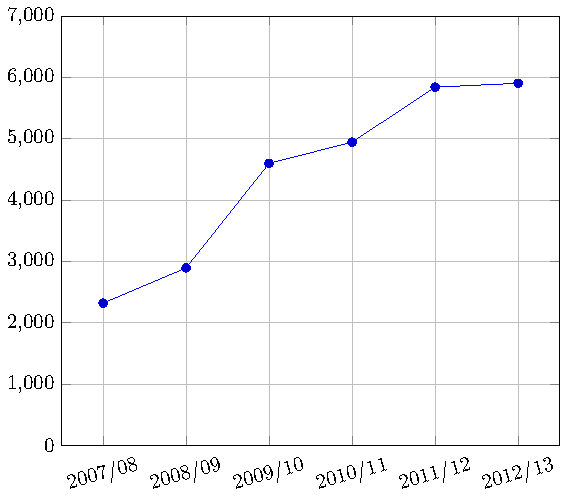
\includegraphics[width=\textwidth]{graphics/enrollmentInDL.pdf}
          % arara: pdflatex
% !arara: indent: {overwrite: yes}
\documentclass{standalone}
% Caption: Enrollment in DL
% 2007/08-2012/13

\usepackage{pgfplots}
\usepackage{pgfplotstable}
\pgfplotsset{compat=newest}


\begin{document}

% http://tex.stackexchange.com/questions/128468/problems-with-pgfplotstableread-and-relative-paths
\IfStandalone{
	\newcommand{\fromRoot}[1]{../data/#1}
	}{
	\newcommand{\fromRoot}[1]{./data/#1}
}

% need to have the read command in the main document, otherwise it will 
% be ignored when used with standalone
\pgfplotstableread[col sep=comma]{\fromRoot{ProcessedGradesData.csv}}\enrollmentdata

\begin{tikzpicture}
	\begin{axis}[
			%ybar,
			symbolic x coords={2007/08, 2008/09, 2009/10, 2010/11, 2011/12, 2012/13, NaN},
			xtick=data,
			minor ytick={1000,2000,...,7000},
			enlarge x limits,
			%scale only axis,       
			grid = both,
			ymin=0,ymax=7000,
			scaled ticks=false, 
			tick label style={/pgf/number format/fixed},
			legend pos=outer north east,
			restrict x to domain=0:5,
			x tick label style={rotate=25},
			width=\textwidth,
		]
		\addplot table[x=AY,y=DL_Enrollments]{\enrollmentdata};
		%\legend{DL}
	\end{axis}
\end{tikzpicture}
\end{document}

          \caption{Enrollments in DL}\label{fig:sec3:DLenrollments}
    \end{minipage}%
    \begin{minipage}{.5\textwidth}
          %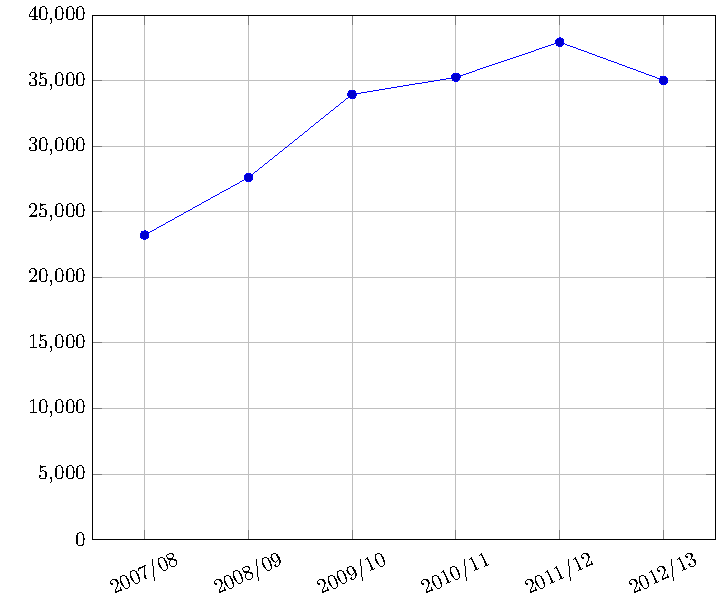
\includegraphics[width=\textwidth]{graphics/enrollmentInF2F.pdf}
          % arara: pdflatex
% !arara: indent: {overwrite: yes}
\documentclass{standalone}
% Caption: Enrollment in F2F
% 2007/08-2012/13

\usepackage{pgfplots}
\usepackage{pgfplotstable}
\pgfplotsset{compat=newest}

\pgfplotstableread[col sep=comma]{../data/ProcessedGradesData.csv}\enrollmentdata

\begin{document}

\begin{tikzpicture}
	\begin{axis}[
			%ybar,
			symbolic x coords={2007/08, 2008/09, 2009/10, 2010/11, 2011/12, 2012/13, NaN},
			xtick=data,
			%minor ytick={1000,5000,...,40000},
			enlarge x limits,
			scale only axis,       
			grid = both,
			ymin=0,ymax=40000,
			scaled ticks=false, 
			tick label style={/pgf/number format/fixed},
			legend pos=outer north east,
			restrict x to domain=0:5,
			x tick label style={rotate=15},
		]
		\addplot table[x=AY,y=F2F_Enrollments]{\enrollmentdata};
		%\legend{DL}
	\end{axis}
\end{tikzpicture}
\end{document}

          \caption{Enrollments in face-to-face classes}\label{fig:sec3:F2Fenrollments}
    \end{minipage}
\end{figure}

\begin{table}[!htb]
	\begin{widepage}
	\centering
  	\caption{DL \& Face-to-face (F2F) enrollments and pass rates 2007--2010}
    \label{tab:sec3:F2FandDLdata2007}
          % arara: pdflatex
\documentclass[varwidth]{standalone}
\usepackage{pgfplotstable}
\usepackage{booktabs}
\usepackage{multirow}

% caption: pass rates by class for DL vs F2F 2007-2008

% empty column type- very useful
\newcolumntype{H}{>{\setbox0=\hbox\bgroup}c<{\egroup}@{}}

\pgfplotstableset{percentstyle/.style={
    preproc/expr={##1*100},
    dec sep align,fixed,fixed zerofill,
postproc cell content/.append code={
            \ifx\\##1\\% check if ##1 is empty
            \else
            \ifnum1=\pgfplotstablepartno
                \pgfkeysalso{@cell content/.add={}{\,\%}}%
            \fi
            \fi
        },
    precision=0,
}
}

% references:
%   http://tex.stackexchange.com/questions/65760/pgfplotstable-how-can-i-add-percent-signs-and-respect-dec-sep-align
%   http://tex.stackexchange.com/questions/16604/easiest-way-to-delete-a-column/16607#16607
%   http://tex.stackexchange.com/questions/89365/check-for-empty-macro-argument

\begin{document}

% http://tex.stackexchange.com/questions/128468/problems-with-pgfplotstableread-and-relative-paths
\IfStandalone{
	\newcommand{\fromRoot}[1]{../data/#1}
	}{
	\newcommand{\fromRoot}[1]{./data/#1}
}

\pgfplotstableread[col sep=comma]{\fromRoot{dlvsF2FenrollmentPassRates.csv}}\dlvsftofdata

\pgfplotstabletypeset[
every head row/.style={
        before row={%
        \toprule
        \multirow{2}{*}{Course}
        & \multicolumn{7}{c}{2007--2008} 
        & \multicolumn{7}{c}{2008--2009} 
        & \multicolumn{22}{c}{2009--2010} 
        \\},
        after row=\midrule},
every last row/.style={after row=\bottomrule},
columns/Course/.style={string type,column name={},column type=r},
    % 2007-08
    % 2007-08
    % 2007-08
    columns/2007-08/.style={column type=H},
    columns/DL2007-08/.style={column name={DL},column type=r},
    columns/DL Pass rate2007-08/.style={column name={\% Pass},percentstyle},
    columns/FtoF2007-08/.style={column name={F2F},column type=r},
    columns/FtoF Pass rate2007-08/.style={column name={\% Pass},percentstyle},
    % 2008-09
    % 2008-09
    % 2008-09
    columns/2008-09/.style={column type=H},
    columns/DL2008-09/.style={column name={DL},column type=r},
    columns/DL Pass rate2008-09/.style={column name={\% Pass},percentstyle},
    columns/FtoF2008-09/.style={column name={F2F},column type=r},
    columns/FtoF Pass rate2008-09/.style={column name={\% Pass},percentstyle},
    % 2009-10
    % 2009-10
    % 2009-10
    columns/2009-10/.style={column type=H},
    columns/DL2009-10/.style={column name={DL},column type=r},
    columns/DL Pass rate2009-10/.style={column name={\% Pass},percentstyle},
    columns/FtoF2009-10/.style={column name={F2F},column type=r},
    columns/FtoF Pass rate2009-10/.style={column name={\% Pass},percentstyle},
    % 2010-11
    % 2010-11
    % 2010-11
    columns/2010-11/.style={column type=H},
    columns/DL2010-11/.style={column type=H},
    columns/DL Pass rate2010-11/.style={column type=H},
    columns/FtoF2010-11/.style={column type=H},
    columns/FtoF Pass rate2010-11/.style={column type=H},
    % 2011-12
    % 2011-12
    % 2011-12
    columns/2011-12/.style={column type=H},
    columns/DL2011-12/.style={column type=H},
    columns/DL Pass rate2011-12/.style={column type=H},
    columns/FtoF2011-12/.style={column type=H},
    columns/FtoF Pass rate2011-12/.style={column type=H},
    % 2012-13
    % 2012-13
    % 2012-13
    columns/2012-13/.style={column type=H},
    columns/DL2012-13/.style={column type=H},
    columns/DL Pass rate2012-13/.style={column type=H},
    columns/FtoF2012-13/.style={column type=H},
    columns/FtoF Pass rate2012-13/.style={column type=H},
    % ignore these columns
    columns/2008-09/.style={column type=H},
    columns/2009-10/.style={column type=H},
    columns/2010-11/.style={column type=H},
    columns/2011-12/.style={column type=H},
    columns/2012-13/.style={column type=H},
]{\dlvsftofdata}

\end{document}

          \vspace{2pc}
  	\caption{DL \& Face-to-face (F2F) enrollments and pass rates 2010--2013}
    \label{tab:sec3:F2FandDLdata2010}
          % arara: pdflatex
\documentclass[varwidth]{standalone}
\usepackage{pgfplotstable}
\usepackage{booktabs}
\usepackage{multirow}

% caption: pass rates by class for DL vs F2F 2010-2013

% empty column type- very useful
\newcolumntype{H}{>{\setbox0=\hbox\bgroup}c<{\egroup}@{}}

\pgfplotstableset{percentstyle/.style={
    preproc/expr={##1*100},
    dec sep align,fixed,fixed zerofill,
postproc cell content/.append code={
            \ifx\\##1\\% check if ##1 is empty
            \else
            \ifnum1=\pgfplotstablepartno
                \pgfkeysalso{@cell content/.add={}{\,\%}}%
            \fi
            \fi
        },
    precision=0,
}
}

% references:
%   http://tex.stackexchange.com/questions/65760/pgfplotstable-how-can-i-add-percent-signs-and-respect-dec-sep-align
%   http://tex.stackexchange.com/questions/16604/easiest-way-to-delete-a-column/16607#16607
%   http://tex.stackexchange.com/questions/89365/check-for-empty-macro-argument

\begin{document}

% http://tex.stackexchange.com/questions/128468/problems-with-pgfplotstableread-and-relative-paths
\IfStandalone{
	\newcommand{\fromRoot}[1]{../data/#1}
	}{
	\newcommand{\fromRoot}[1]{./data/#1}
}

\pgfplotstableread[col sep=comma]{\fromRoot{dlvsF2FenrollmentPassRates.csv}}\dlvsftofdata


\pgfplotstabletypeset[
every head row/.style={
        before row={%
        \toprule
        \multirow{2}{*}{Course}
        & \multicolumn{22}{c}{2010--2011} 
        & \multicolumn{7}{c}{2011--2012} 
        & \multicolumn{7}{c}{2012--2013} 
        \\},
        after row=\midrule},
every last row/.style={after row=\bottomrule},
columns/Course/.style={string type,column name={},column type=r},
    % 2007-08
    % 2007-08
    % 2007-08
    columns/2007-08/.style={column type=H},
    columns/DL2007-08/.style={column type=H},
    columns/DL Pass rate2007-08/.style={column type=H},
    columns/FtoF2007-08/.style={column type=H},
    columns/FtoF Pass rate2007-08/.style={column type=H},
    % 2008-09
    % 2008-09
    % 2008-09
    columns/2008-09/.style={column type=H},
    columns/DL2008-09/.style={column type=H},
    columns/DL Pass rate2008-09/.style={column type=H},
    columns/FtoF2008-09/.style={column type=H},
    columns/FtoF Pass rate2008-09/.style={column type=H},
    % 2009-10
    % 2009-10
    % 2009-10
    columns/2009-10/.style={column type=H},
    columns/DL2009-10/.style={column type=H},
    columns/DL Pass rate2009-10/.style={column type=H},
    columns/FtoF2009-10/.style={column type=H},
    columns/FtoF Pass rate2009-10/.style={column type=H},
    % 2010-11
    % 2010-11
    % 2010-11
    columns/2010-11/.style={column type=H},
    columns/DL2010-11/.style={column name={DL},column type=r},
    columns/DL Pass rate2010-11/.style={column name={\% Pass},percentstyle},
    columns/FtoF2010-11/.style={column name={F2F},column type=r},
    columns/FtoF Pass rate2010-11/.style={column name={\% Pass},percentstyle},
    % 2011-12
    % 2011-12
    % 2011-12
    columns/2011-12/.style={column type=H},
    columns/DL2011-12/.style={column name={DL},column type=r},
    columns/DL Pass rate2011-12/.style={column name={\% Pass},percentstyle},
    columns/FtoF2011-12/.style={column name={F2F},column type=r},
    columns/FtoF Pass rate2011-12/.style={column name={\% Pass},percentstyle},
    % 2012-13
    % 2012-13
    % 2012-13
    columns/2012-13/.style={column type=H},
    columns/DL2012-13/.style={column name={DL},column type=r},
    columns/DL Pass rate2012-13/.style={column name={\% Pass},percentstyle},
    columns/FtoF2012-13/.style={column name={F2F},column type=r},
    columns/FtoF Pass rate2012-13/.style={column name={\% Pass},percentstyle},
    % ignore these columns
    columns/2008-09/.style={column type=H},
    columns/2009-10/.style={column type=H},
    columns/2010-11/.style={column type=H},
    columns/2011-12/.style={column type=H},
    columns/2012-13/.style={column type=H},
]{\dlvsftofdata}

\end{document}

          \end{widepage}
\end{table}

As enrollment demand for DL math courses has increased, we have increased the
number of sections that we offer and trained more interested faculty in managing
DL courses.  Between the academic years of 2003/04 and 2007/08, the annual
number of sections offered increased from 51 to 87.  In the 2012/13 academic
year, we offered 185 DL sections.   The resulting increase in sections offers
access to students that can succeed in this modality and need this option due to
outside constraints such as work and family.


\subsection{Success rates in DL courses}
Pass rates in DL courses are quite noticeably lower than those for their
face-to-face counterparts. \Cref{fig:sec3:F2FandDLpassRates} visualizes the
difference in pass rates between the highest enrollment DL courses that we offer
and their face-to-face counterparts. More detailed data for all DL offerings can
be seen in \cref{tab:sec3:F2FandDLdata2007,tab:sec3:F2FandDLdata2010}. We recognize that students need a
certain level of self-discipline, better study skills, and comfort engaging with
technology to succeed in a DL course. However we currently have no method for
screening which students are less likely to succeed using a distance modality;
our recommendations on \cpageref{other:sec:recommendations} attempt to address this issue.


Referencing \cref{fig:sec3:F2FandDLpassRates}, 
it is clear that, in the six academic years shown, the pass rates 
generally decrease regardless of delivery mode.  We hypothesize that this
overall trend is mostly the result of the economic collapse of 2008 which led to
increased enrollment and changes in our student demographics (see demographics
data in \vref{app:sec:demographicdata}).  But the pass rates in DL courses are
as much as 30\% lower than in face-to-face counterparts and this large
discrepancy needs to be addressed.

\begin{figure}[!htb]
  \begin{widepage}
    \begin{subfigure}{.3\textwidth}
          % arara: pdflatex
% !arara: indent: {overwrite: yes}
\documentclass{standalone}
% Caption: Enrollment in DL
% 2007/08-2012/13

\usepackage{pgfplots}
\usepackage{pgfplotstable}
\pgfplotsset{compat=newest}

\pgfplotstableread[col sep=comma]{../data/ProcessedGradesData.csv}\enrollmentdata

\begin{document}

\begin{tikzpicture}
	\begin{axis}[
			%ybar,
			symbolic x coords={2007/08, 2008/09, 2009/10, 2010/11, 2011/12, 2012/13, NaN},
			xtick=data,
			%minor ytick={1000,2000,...,7000},
			enlarge x limits,
			scale only axis,       
			grid = both,
			ymin=0.3,ymax=0.85,
			axis y discontinuity=crunch,
			scaled ticks=false, 
			tick label style={/pgf/number format/fixed},
			legend pos=outer north east,
			restrict x to domain=0:5,
			x tick label style={rotate=15},
		]
		\addplot table[x=AY,y=020_DL_Pass_Rate]{\enrollmentdata};
		\addplot table[x=AY,y=020_F2F_Pass_Rate]{\enrollmentdata};
		\legend{DL 020, F2F 020}
	\end{axis}
\end{tikzpicture}
\end{document}

          \captionof{figure}{MTH 20}
    \end{subfigure}%
    \begin{subfigure}{.3\textwidth}
          % arara: pdflatex
% !arara: indent: {overwrite: yes}
\documentclass{standalone}
% Caption: Enrollment in DL
% 2007/08-2012/13

\usepackage{pgfplots}
\usepackage{pgfplotstable}
\pgfplotsset{compat=newest}

\pgfplotstableread[col sep=comma]{../data/ProcessedGradesData.csv}\enrollmentdata

\begin{document}

\begin{tikzpicture}
	\begin{axis}[
			%ybar,
			symbolic x coords={2007/08, 2008/09, 2009/10, 2010/11, 2011/12, 2012/13, NaN},
			xtick=data,
			%minor ytick={1000,2000,...,7000},
			enlarge x limits,
			scale only axis,       
			grid = both,
			ymin=0.3,ymax=0.85,
			axis y discontinuity=crunch,
			scaled ticks=false, 
			tick label style={/pgf/number format/fixed},
			legend pos=outer north east,
			restrict x to domain=0:5,
			x tick label style={rotate=15},
		]
		\addplot table[x=AY,y=060_DL_Pass_Rate]{\enrollmentdata};
		\addplot table[x=AY,y=060_F2F_Pass_Rate]{\enrollmentdata};
		\legend{DL 060, F2F 060}
	\end{axis}
\end{tikzpicture}
\end{document}

          \captionof{figure}{MTH 60}
    \end{subfigure}%
    \begin{subfigure}{.3\textwidth}
          % arara: pdflatex
% !arara: indent: {overwrite: yes}
\documentclass{standalone}
% Caption: Enrollment in DL
% 2007/08-2012/13

\usepackage{pgfplots}
\usepackage{pgfplotstable}
\pgfplotsset{compat=newest}


\begin{document}

% http://tex.stackexchange.com/questions/128468/problems-with-pgfplotstableread-and-relative-paths
\IfStandalone{
	\newcommand{\fromRoot}[1]{../data/#1}
	}{
	\newcommand{\fromRoot}[1]{./data/#1}
}
\pgfplotstableread[col sep=comma]{\fromRoot{ProcessedGradesData.csv}}\enrollmentdata

\begin{tikzpicture}
	\begin{axis}[
			%ybar,
			symbolic x coords={2007/08, 2008/09, 2009/10, 2010/11, 2011/12, 2012/13, NaN},
			xtick=data,
			%minor ytick={1000,2000,...,7000},
			enlarge x limits,
			%scale only axis,       
			grid = both,
			ymin=0.3,ymax=0.85,
			axis y discontinuity=crunch,
			scaled ticks=false, 
			tick label style={/pgf/number format/fixed},
			legend pos=south west,
			restrict x to domain=0:5,
			x tick label style={rotate=25},
            width=\textwidth,
		]
		\addplot table[x=AY,y=065_DL_Pass_Rate]{\enrollmentdata};
		\addplot table[x=AY,y=065_F2F_Pass_Rate]{\enrollmentdata};
		\legend{DL 065, F2F 065}
	\end{axis}
\end{tikzpicture}
\end{document}

          \captionof{figure}{MTH 65}
    \end{subfigure}

\vspace{2pc}

    \begin{subfigure}{.3\textwidth}
          % arara: pdflatex
% !arara: indent: {overwrite: yes}
\documentclass{standalone}
% Caption: Enrollment in DL
% 2007/08-2012/13

\usepackage{pgfplots}
\usepackage{pgfplotstable}
\pgfplotsset{compat=newest}


\begin{document}
% http://tex.stackexchange.com/questions/128468/problems-with-pgfplotstableread-and-relative-paths
\IfStandalone{
	\newcommand{\fromRoot}[1]{../data/#1}
	}{
	\newcommand{\fromRoot}[1]{./data/#1}
}
\pgfplotstableread[col sep=comma]{\fromRoot{ProcessedGradesData.csv}}\enrollmentdata

\begin{tikzpicture}
	\begin{axis}[
			%ybar,
			symbolic x coords={2007/08, 2008/09, 2009/10, 2010/11, 2011/12, 2012/13, NaN},
			xtick=data,
			%minor ytick={1000,2000,...,7000},
			enlarge x limits,
			%scale only axis,       
			grid = both,
			ymin=0.3,ymax=0.85,
			axis y discontinuity=crunch,
			scaled ticks=false, 
			tick label style={/pgf/number format/fixed},
			legend pos=north east,
			restrict x to domain=0:5,
			x tick label style={rotate=25},
            width=\textwidth,
		]
		\addplot table[x=AY,y=095_DL_Pass_Rate]{\enrollmentdata};
		\addplot table[x=AY,y=095_F2F_Pass_Rate]{\enrollmentdata};
		\legend{DL 095, F2F 095}
	\end{axis}
\end{tikzpicture}
\end{document}

          \captionof{figure}{MTH 95}
    \end{subfigure}%
    \begin{subfigure}{.3\textwidth}
          % arara: pdflatex
% !arara: indent: {overwrite: yes}
\documentclass{standalone}
% Caption: Enrollment in DL
% 2007/08-2012/13

\usepackage{pgfplots}
\usepackage{pgfplotstable}
\pgfplotsset{compat=newest}

\pgfplotstableread[col sep=comma]{../data/ProcessedGradesData.csv}\enrollmentdata

\begin{document}

\begin{tikzpicture}
	\begin{axis}[
			%ybar,
			symbolic x coords={2007/08, 2008/09, 2009/10, 2010/11, 2011/12, 2012/13, NaN},
			xtick=data,
			%minor ytick={1000,2000,...,7000},
			enlarge x limits,
			scale only axis,       
			grid = both,
			ymin=0.3,ymax=0.85,
			axis y discontinuity=crunch,
			scaled ticks=false, 
			tick label style={/pgf/number format/fixed},
			legend pos=outer north east,
			restrict x to domain=0:5,
			x tick label style={rotate=15},
		]
		\addplot table[x=AY,y=111_DL_Pass_Rate]{\enrollmentdata};
		\addplot table[x=AY,y=111_F2F_Pass_Rate]{\enrollmentdata};
		\legend{DL 111, F2F 111}
	\end{axis}
\end{tikzpicture}
\end{document}

          \captionof{figure}{MTH 111}
    \end{subfigure}%
    \begin{subfigure}{.3\textwidth}
          % arara: pdflatex
% !arara: indent: {overwrite: yes}
\documentclass{standalone}
% Caption: Enrollment in DL
% 2007/08-2012/13

\usepackage{pgfplots}
\usepackage{pgfplotstable}
\pgfplotsset{compat=newest}

\pgfplotstableread[col sep=comma]{../data/ProcessedGradesData.csv}\enrollmentdata

\begin{document}

\begin{tikzpicture}
	\begin{axis}[
			%ybar,
			symbolic x coords={2007/08, 2008/09, 2009/10, 2010/11, 2011/12, 2012/13, NaN},
			xtick=data,
			%minor ytick={1000,2000,...,7000},
			enlarge x limits,
			scale only axis,       
			grid = both,
			ymin=0.3,ymax=0.85,
			axis y discontinuity=crunch,
			scaled ticks=false, 
			tick label style={/pgf/number format/fixed},
			legend pos=outer north east,
			restrict x to domain=0:5,
			x tick label style={rotate=15},
		]
		\addplot table[x=AY,y=243_DL_Pass_Rate]{\enrollmentdata};
		\addplot table[x=AY,y=243_F2F_Pass_Rate]{\enrollmentdata};
		\legend{DL 243, F2F 243}
	\end{axis}
\end{tikzpicture}
\end{document}

          \captionof{figure}{MTH 243}
    \end{subfigure}
    \caption{Pass Rates By Modality}
    \label{fig:sec3:F2FandDLpassRates}
  \end{widepage}
\end{figure}

The difference in student-success rates between on-campus courses and DL courses
is an important issue for the Math SAC.  The Distance Learning Standing
Committee has met to consider this issue and the factors that lead to this
difference in success rates.  We can only speculate the reason for the disparity
based on anecdotal evidence and professional experience.  Students may no longer
see DL courses as unusual, so they may be unaware that successful DL math
students should have stronger study skills, self-discipline, and time management
skills than face-to-face math students absolutely need to be successful. We
believe that many students register for DL math courses without adequate
understanding of the study habits, time commitment, learning styles, and
technical skills that are necessary for success in these classes. Anecdotal
evidence suggests that some students who are aware of these issues and who would
otherwise enroll in a face-to-face section still enroll in a DL section due to a
lack of space in face-to-face sections.

There is currently a DL orientation available for DL students, but there is no
requirement that students complete it. Furthermore, there is no information in
the orientation to help students understand the particular challenges of
studying \emph{mathematics} using the DL delivery methods.  In many disciplines,
reading, writing, and discussion can be sufficient for learning. Students in
mathematics typically do not learn best until they have also acted, by working
through exercises or active problem-solving. In face-to-face classes,
instructors can monitor that this learning-through-action is happening more
easily. In DL courses, there is more of a need for students to rely on
self-discipline to complete this portion of their learning, and this is not
communicated in the existing DL orientation.


\subsection{Informing DL students}
The Course Information Page (CIP) is accessible to students registering for DL
courses and is meant to give section-specific information to students as they
decide which sections to register for.   Many faculty members use this system to
inform students of issues related to an online mathematics course.  For example,
faculty address the misconception that a DL class requires fewer hours of
attention per week than a face-to-face class. We believe that many students do
not visit the CIP for DL classes and continue to be unaware of the tools they
will need to be successful in a DL mathematics course.   Some faculty members
send emails to registered students before the term starts, asking them to read
the CIP;  it is not clear, however, how many students read this email or act on
it.  The link to a CIP is only available via the online class, and not via
MyPCC; this lack of presence may contribute to the issue.

Other methods that are employed by DL faculty to directly communicate with their
students include:
\begin{itemize}
\item using the Course Progress Notifications (CPNs);
\item placing telephone calls to students;
\item using Collaborate to hold online office hours in a kind of visual and aural chat session.
\end{itemize}

\subsection{Online homework platforms}
Faculty have sought to increase engagement by DL students through use of online
homework platforms. An online homework platform can provide students with
immediate feedback and also hold the student accountable for completion of
assigned exercises. Faculty can monitor progress and employ formative assessment
from a distance.

The SAC recognizes that program changes should come from research toward best
practices.  Faculty members Wendy Fresh, Rebecca Ross, Tammy Louie, Jessica
Bernards, and Diane Edwards have investigated the effects of use of an online
homework system in several experiments in both DL and face-to-face courses. In most
cases, results from these experiments suggest there may be positive effects to
using an online platform, but it remains too early to declare statistical
significance. To demonstrate statistical significance in studies of this nature
requires considerably large sample sizes. 

However Jessica Bernards has been able to measure one positive effect to a
significant degree. Instructor Bernards taught several online sections of MTH
111, with control groups doing homework from the textbook and submitting paper
write-ups, and experimental groups using online homework. The withdrawal rate
was 32\% for the control group and only 16\% for the experimental group, and
this difference was statistically significant ($P<1\%$).  Instructor Wendy Fresh
ran a very similar experiment with online sections of MTH 60. There may still be
an effect at that level, but more data is necessary to confirm with statistical
significance. Both instructors noted modest improvement in exam scores among the
experimental group, but again more data is being gathered to confirm with
significance.

For more information on research by Instructors Bernards and Fresh for DL
courses, see \vref{app:sec:onlinehwstudy}. For information on research by
instructors Edwards and Louie, see \vref{app:sec:aleks} and also
\cpageref{sec3:subset:alekspilot}. Research on the efficacy of WeBWorK (an online
homework platform discussed on \cpageref{other:sec:webwork}) was done in
\cite{focuswebwork}.  In \cite{brewer} it was found that when students are
segregated by incoming ability, those who were less prepared when entering a
course do benefit significantly from online homework use. As a community
college, we have more under prepared students than universities, so this
finding suggests that use of online homework may be more helpful at PCC. It is
important to note that each of these studies were done with face-to-face
courses; in DL courses the traditional homework alternative presents the
challenge of delivery, complicating the question in favor of using online
homework.

\subsection{WeBWorK}\label{other:sec:webwork}
Recent exciting developments at PCC have centered around the free and
open-source online homework platform called WeBWorK that is partially funded by
the National Science Foundation and maintained by the Mathematical Association
of America. By Spring 2014 we expect that over 20 faculty will be using WeBWorK
in their courses. The math SAC is also loaning out the services of Alex Jordan
to CTE and LDC science SACs to create free online homework review programs. We
envision using WeBWorK for future Learning Assessment research and placement
advising. We are working with Dual Credit instructors to offer WeBWorK services
to Portland Public Schools.

Most of the textbooks currently in use by the Math SAC are published by Pearson
Publishing, which offers MyMathLab for its online homework platform. While
MyMathLab and similar commercial products come as a bundled expense with new
textbook purchases, a separate online account for pairing with a used textbook
purchase is rather expensive. For this reason, face-to-face instructors rarely
require MyMathLab in their courses. On the other hand, Distance Learning
instructors have a stronger need for an online homework platform and the
majority of DL instructors do require that students use (and pay for) MyMathLab.

By contrast, WeBWorK is a platform for online homework that is free and
open-source. As there is no central headquarters for WeBWorK, it must be
installed on a server somewhere. Since joining the Math SAC in Spring 2009,
Alex Jordan has championed the implementation and use of WeBWorK at PCC. Some
PCC math faculty have used WeBWorK in various capacities by borrowing server
space from the University of Oregon, a relationship formed and maintained by
Jordan. This partnership between two Oregon state institutions has been
mutually beneficial. While PCC gained server access, PCC faculty members were
programming content that the University of Oregon has been able to take advantage of. Each term since
Fall 2011, roughly 10 sections of PCC math courses have used the UO server.

Over this period, WeBWorK users in the Math SAC lobbied Technology Solution
Services to provide the Math SAC with its own WeBWorK server. While the UO
server provided service to us, it came with certain restrictions and
complications that prevented WeBWorK at PCC from reaching its full potential.
For a time there was a chicken-and-egg situation, as TSS requested a greater
usage by PCC faculty before arranging for a server while some faculty chose not
to use WeBWorK because of the inconvenience of using the UO server.

In the 2012/13 academic year, faculty Chris Hughes and Scot Leavitt researched
accessibility issues (in the ADA sense) alongside Disability Services. See
\cite{accessibilityproject} for the full report. Among many other findings, they
found that MyMathLab (at the time of the project) had many significant
accessibility problems while WeBWorK was quite close to being fully ADA
compliant. The open-source nature of WeBWorK meant that the few remaining
obstacles to accessibility could be addressed. They recommended that the SAC
cease using MyMathLab for newly developed courses and newly developed online
shells. They also recommended that faculty migrate from MyMathLab to WeBWorK.
Disability Services supported their recommendations, and also began lobbying TSS
for a PCC WeBWorK server. Within the WeBWorK community PCC is now seen as a
leader when it comes to accessibility issues. See \cite{webworkblog} for a post
about this on the WeBWorK news blog. As a result of this, PCC is hosting a
WeBWorK development camp in August 2014 with a central theme of addressing
accessibility issues and enhancing its accessibility.\label{other:page:disabilityservices}

TSS partnered with the Clackamas Education Service District to deliver a WeBWorK
server that has been fully implemented since Winter 2014.  SAC members Alex Jordan,
Chris Hughes, and Xiaolong Yao have prepared
\href{http://webwork.pcc.edu}{webwork.pcc.edu} for regular use starting Winter
2014 term. A backup server at
\href{http://webwork-dev.pcc.edu}{webwork-dev.pcc.edu} is in place for faculty
to experiment with. 

The arrival of our own WeBWorK installation has significant implications beyond
homework management, particularly in the advising department. We envisage that
advisors would enroll students in a `review course' that contains (mostly)
pre-college practice problems, and that the student would be encouraged to sit
the COMPASS placement test only when they are comfortable with the problems in
WeBWorK. Furthermore, we can easily use WeBWorK as an advising tool to replace
Hughes' Placement Advisory Test (\cite{mathprogramreview2003}, pages 12--13) in situations when students are not happy with
their placement from COMPASS.  The SAC should work with advising to implement
this. 

\subsection{PCC WeBWorK problem library}
WeBWorK has been in use at universities for some time now, and an extensive
library exists of math problems for college-level courses. However there was
weak content support for basic algebra and other pre-college topics. Over Summer 2013, Alex Jordan, Chris Hughes, and Xiaolong Yao oversaw an effort to create
a library of high-quality, algorithmically generated, basic algebra WeBWorK
exercises which was partly funded with an IIP development grant; they received
support from math instructors Kandace Kling, Debbie Neft, Jeremy Shaw, and Danielle Rice.  These
exercises currently cover topics from MTH 60 and 65, and the team continues to
add problems to the library for MTH 95. The library development was a success
because of the strong collaboration and dedication of the three faculty members,
and the foundations that Jordan had laid in previous years. Jordan, Hughes,
and Yao presented their work at the STEM showcase (Rock Creek) in Fall 2013 (see
\cref{webworkposter}). It was at this showcase that the idea was hatched to
create free online homework review programs for CTE and LDC science SACs.

\begin{figure}[!htb]
	\centering
	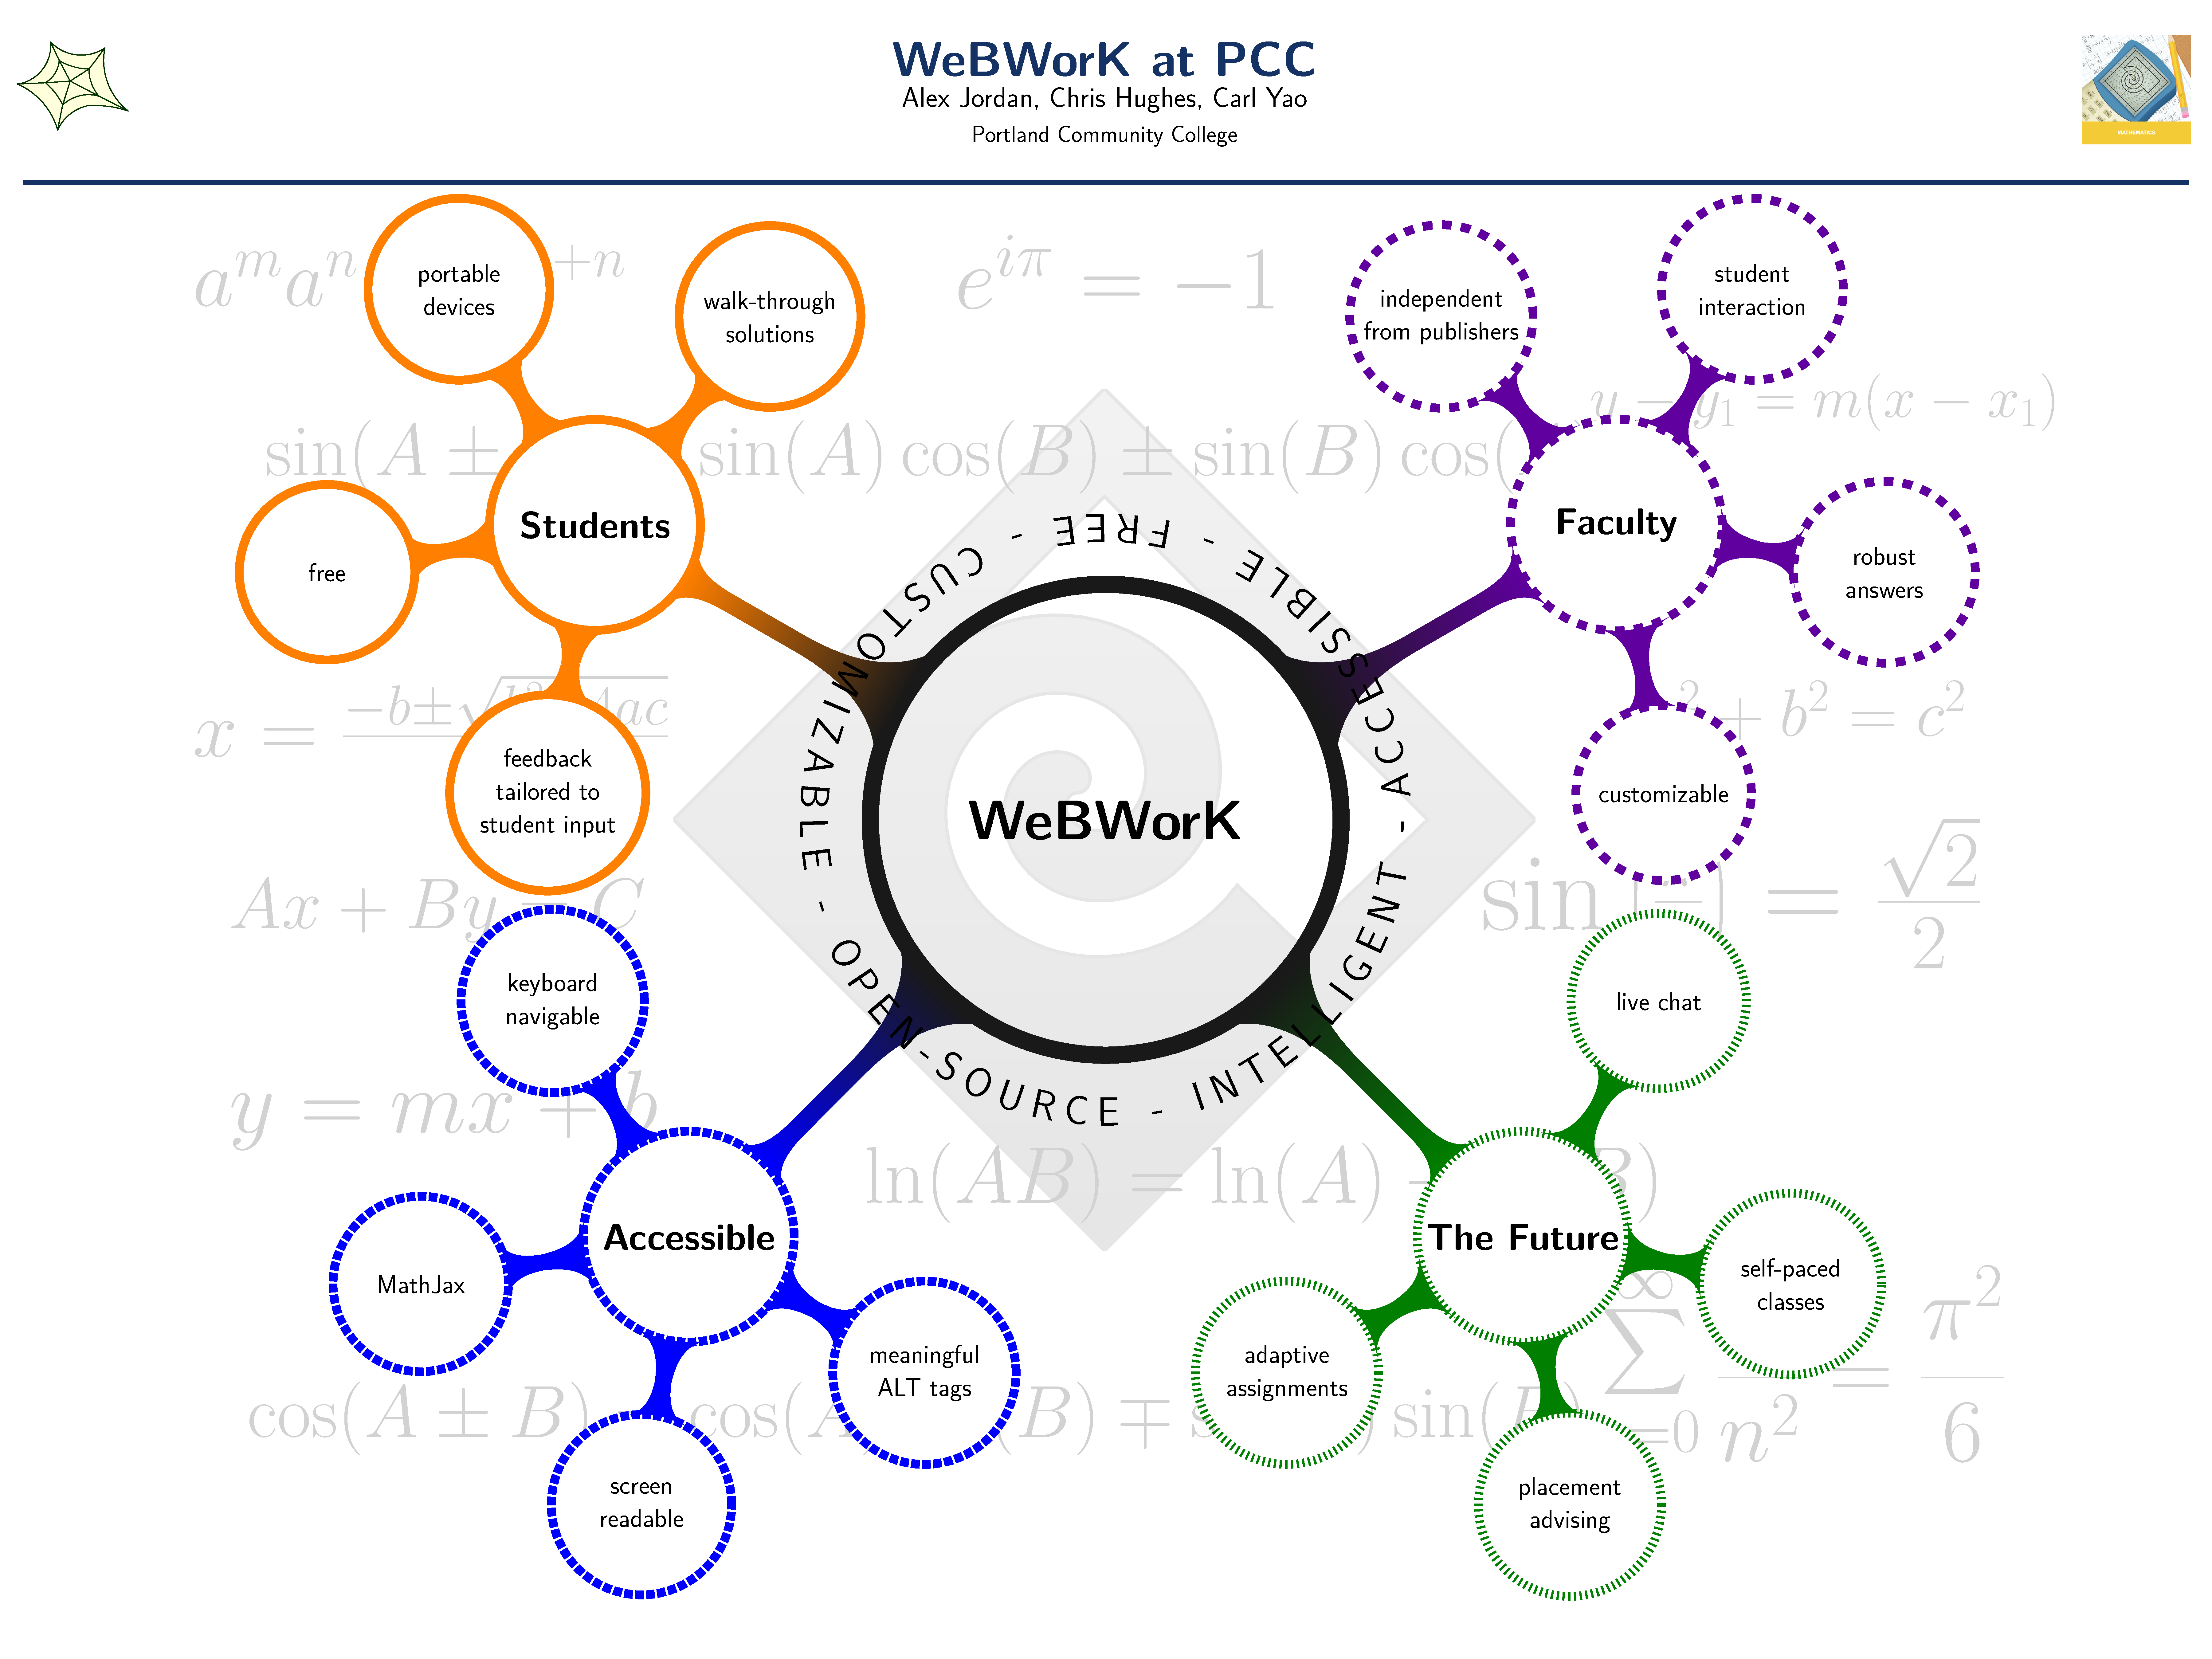
\includegraphics[width=0.5\textwidth]{webworkposter.pdf}
	\caption{WeBWorK poster from the PCC STEM Showcase}\label{webworkposter}
\end{figure}

As time and funding progress, SAC members with the requisite coding experience
hope to add more problems to this PCC library, expanding into the arenas of MTH
courses 20, 111, 112, 243, and 244. It is important to note the level of quality
of the problems from this library. Each problem has a full walk-through solution
coded along side the question which can be put to use by faculty in a number of
ways. Each problem is given fine attention to detail so that automated feedback
messages to the students are as informative as modern technology can allow. This
high level of quality requires time and experience to achieve. However it is
necessary if any instructor hopes to use WeBWorK as a teaching tool and not just
an assessment tool.

\subsection{Concerns about DL offerings}
Each of the following three issues have been raised by SAC members, and during
the 2012/13 academic year a group of concerned faculty met to discuss them. The
meetings were informal and no binding decisions were reached.
\begin{itemize}
\item Faculty are concerned about whether or not Distance Learning is an
  effective way to deliver math content, especially in light of the low pass
  rate statistics seen in \cref{fig:sec3:F2FandDLpassRates}. Successfully
  learning mathematics generally requires heavy active engagement. Face-to-face
  courses facilitate this engagement by requiring students to be in the physical
  presence of their instructor and fellow students. In DL courses, the
  imperative to remain engaged must come mostly from the student's own sense of
  responsibility and interest.
\item Faculty are concerned about the quality and consistency of current DL
  courses. Some faculty rely on publisher content such as electronic versions of
  textbooks, while other faculty have created complete sets of online notes
  themselves and use e-books only as secondary resources. Instructor Chris
  Hughes serves as an advisor to online faculty creating new courses, and makes
  recommendations to improve course quality and observe accessibility standards.
  However there is no enforcement of the online advisor's recommendations.
\item Faculty are concerned about the portion of a student's grade that may be
  computed from online homework. Compared to traditional homework, online
  homework is more readily vulnerable to cheating. With many math exercises, the
  exercise can literally be typed in to Google and the search engine itself
  provides an answer. Online homework provides fewer obstacles for a dishonest
  student to employ someone else to do their homework for them. In fact, in
  Craigslist sites nationwide, all one need do is search for `mymathlab' to find
  advertisements from those who will `take your online math course for you' at a
  cost. The math SAC has always wanted its online courses to mirror its
  face-to-face courses, and as a consequence has never created CCOGs that treat
  face-to-face and online courses differently. This has made it difficult to
  place any cap on the portion of a grade that may be computed from online
  homework. There is also no consensus on what an appropriate cap would be.
\end{itemize}

\subsection{Recommendations}\label{other:sec:recommendations}
\recommendation{Our main recommendations concern how to best inform students about the
particular skills that a distance learning student should have or adopt in order
to be successful. We also recommend enacting some prerequisite items for DL
registration to help give these skills to students. Lastly there are some
recommendations that do not fit these descriptions. Many of these
recommendations hold for face-to-face courses as well, and may be repeated elsewhere in
this program review.}
\begin{description}
\item For the Math SAC:
\begin{itemize}[label={}]
\item \recommendation{Collaborate with advising to implement a WeBWorK-based review mechanism
  for would-be placement test-takers.}
\item \recommendation{Consider how the quality of online courses could be improved by more effective regulation by the SAC. }
\end{itemize}
\item For Administration/Advising:
\begin{itemize}[label={}]
\item \recommendation{Collaborate with the Math SAC to implement a WeBWorK-based review
  mechanism for would-be placement test-takers.}
\item \recommendation{Give students more information on DL responsibilities and make students
  aware of the difference in student-success statistics between DL and face to
  face courses.}
\item \recommendation{Encourage students to contemplate why they seek to take a DL course and
  reflect upon whether it will align well with their learning style and
  personal skill sets.}
\end{itemize}
\item For Administration/DL/TSS:
\begin{itemize}[label={}]
\item \recommendation{Have the online orientation linked from the registration tool in MyPCC and
  require that students complete this orientation before registering for a DL
  class.}
\item \recommendation{Include a section in the DL orientation that addresses the specific
  challenges that DL brings to mathematics courses. Perhaps only students
  seeking to register for a mathematics DL course would be required to complete
  this section.}
\item \recommendation{Add redundant access to the Course Information Page. Along with access
  through the online Class Schedule, the CIP could be available through MyPCC on
  the home page for a course and through Desire To Learn.}
\item \recommendation{Include a pop-up or hover-over window that is activated when a student
  tries to register for a DL MTH class that gives specific information about the
  challenges of DL Math courses. }
\end{itemize}
\item For Administration/Other:
\begin{itemize}[label={}]
\item \recommendation{Require students to demonstrate pre-requisite computer literacy skills
  such as those taught in basic internet skills (CAS 104), beginning Word (CAS
  216), beginning keyboard (CAS 121), and basic computer skills/MS Office (CAS
  133).}
\item \recommendation{Develop and require a basic DL/computer skills competency course, possibly
  offered during week 0 of the term.  }
\item \recommendation{Provide opportunities for faculty professional development in research
  design and data analysis to help with research efforts on the efficacy of
  online homework.}
\item \recommendation{Provide support for further development of WeBWorK related projects,
  including a larger library of math problems for courses beyond 60/65/95,
  enhancements of the WeBWorK engine, and content for placement advising/review.}
\end{itemize}
\end{description}

\section[Curricular changes resulting from educational initiatives]{Has the SAC
made any curricular changes as a result of exploring/adopting educational
initiatives (e.g., Service Learning, Internationalization of the Curriculum,
Inquiry-Based Learning, Honors, etc.)?  If so, please describe.}


\subsection{Math 111H College Algebra: Honors}\label{cur:sub:111H}

The course has been offered only at Sylvania campus---Winter 2012 (12
students), Winter 2013 (22 students), Spring 2013 (15 students), and Fall 2013
(17 students).  Ronda Lively was the instructor the first three terms, which
allowed her to evolve her materials and activities.  Ann Cary taught the
Fall 2013 term, and has collaborated closely with Ronda Lively. 

The honors course must cover the same material as the regular course. It
is stressed that honors versions of a course should not be ``harder'', but
different in the use of class time and activities/assignments.  There should
also be a component of Community and Environmental Responsibility, which is a
PCC core outcome that is usually difficult to place in math courses.  Instructor
Lively regularly teaches MTH 111 and MTH 111H during the same term.  The same
exams were given in both courses.  There were differences in the other evaluation
criteria used in the courses.  In the MTH 111 class, students submitted take
home graded worksheets and participated in an in-class graded group activity.
The evaluation of the students in the MTH 111H class included:
\begin{itemize}
\item a collaborative computer project involving math history and investigation
  of several applications of math
\item a team quiz-grading activity where each group wrote a key and grading
  rubric, then applied it to two (fictional) students' quizzes
\item a community tutoring project:  over several weeks, each student found someone to
  tutor in math (friend, neighbor, family member, \ldots) and then wrote a paper
  on their experience
\end{itemize}
Since the overall student ability level was high, there was time in class to
investigate other topics of interest related to college algebra.  Each term
there were several students that enrolled because of the time slot,
not because they were strong in math.  Encouragingly, the
stronger students took the less prepared students under their wings and helped
them to be successful.


\subsection{Social justice workgroup}\label{cur:sub:socialJustic}
A Math and Social Justice workgroup was formed by Ann Cary and Emiliano Vega in
response to a national convention they attended. The group has collected and
disseminated data sets and activities to participating math instructors and has
gained interest and participants from other disciplines at PCC, as well as area
high school math instructors and community activists in Portland. More
importantly, the group has the focus of providing a forum on how to discuss
potentially sensitive subjects in a classroom setting when using application
problems and how to be more culturally and socially aware of individual students
and classes. The information they gathered has improved the pool of activities and application problems
available, improved the ability of instructors to work effectively with the
broad demographic of students and co-workers, and also continues the college's
focus on two Core Outcomes: Community and Environmental Responsibility and
Cultural Awareness. For a sample of material from this workgroup, see
\vref{app:sec:socialJustic}.

\subsection{Service learning}\label{other:sec:servicelearning}
Service Learning has been a part of many math instructors' courses at PCC, but
has been deepened through the Service Learning website
which includes additional resources and syllabi submitted
by participating Instructors at PCC. In addition, Service Learning will be
added to some CCOGs evaluation criteria to encourage instructors to incorporate
Service Learning in their math classes. Jeff Pettit participated as
an observer in the Service Learning training cohort at Sylvania campus,
connecting with instructors in other disciplines and gaining an understanding of 
how Service Learning is employed in other courses. This has led to new curriculum in his
Statistics courses and upper-division courses where Service Learning was not
originally employed.

\subsection{Developmental Education math study group}
A new committee was formed by the SAC to address developmental math completion
rates. The committee is researching the feasibility, cost and difficulty
associated with implementing ``pathways'' beyond the current calculus focused
MTH60--95 courses. The committee is considering options for employing
career-based math course series and a statistics-based math course series.

\subsection{Placement test reform group}\label{other:sec:placementreform}
A committee has been formed to address placement test reform. The
group intends to better measure students' needs beyond the current math-skills
COMPASS test. We hope to find a way to measure key traits and needs of students
to connect student populations with the support needed to better guarantee
success.
% I had encouraged these guys to work with student services, who are also
% addressing these concerns.  I don't know if they are or not though.  I do
% know that student services is working with the NSF Grant proposal team on
% these issues.  Perhaps a little more should be said here?

\section[Present dual credit relationships]{Are there any courses in the program
that are offered as Dual Credit at area High Schools?  If so, describe how 
the SAC develops and maintains relationships with the HS faculty in support of
quality instruction. Please note any best practices you have found, or ideas
about how to strengthen this interaction.  }

During the 2012/13 academic year, PCC dual credit was awarded
for seven mathematics courses.  Classes were offered at seven high schools and
there were a total of twelve instructors certified to teach PCC dual credit
mathematics classes.  There were a total of 750 unduplicated students who
enrolled in at least one PCC dual credit mathematics class and collectively
those students earned 6032 mathematics credits through PCC.
In Fall 2012, an ad hoc committee was formed in the mathematics SAC to investigate the status of our dual credit program.  The formation of this committee was prompted, in part, by the discovery that several of the posted dual credit syllabi described courses that bore little resemblance to the course for which students were earning PCC credit.  The committee decided that the root cause of this disconnect was a lack of robust support on our part.  Three concrete actions were taken to address the disconnect:
\begin{itemize}
\item Each dual credit mathematics instructor was assigned a team of two support
  faculty from the mathematics departments at PCC.  Each pair of support faculty
  visited their assigned instructor at that instructor's high school.  These
  meetings were rather informal; the intent being to establish a concrete
  support team for each high school instructor.
\item A two-day mandatory summer workshop was organized by the committee in
  conjunction with Beth Molenkamp, who at that time was the coordinator of
  PCC's dual credit program.  At the workshop each dual credit instructor was
  tasked to complete a robust (and accurate) syllabus for each of their dual
  credit classes.  The PCC faculty helped with this task and all of the dual
  credit instructors now have syllabi that truly reflect the nature of the
  course for which the students are earning PCC credit.  The remainder of the
  workshop was spent sharing resources and pedagogical tactics used by various
  PCC faculty in the courses for which dual credit is also offered.
\item A Google Drive site was created to share resources.  Although the
  inspiration for this site was to give our dual credit faculty easy access to
  shared resources, the pooling of resources is obviously of great benefit for
  PCC faculty as well.
\end{itemize}

\section[Future dual credit relationships]{Does the SAC plan to develop any
additional Dual Credit agreements with area high schools?  If so please
describe.   If not, what does the SAC see as barriers to developing further dual
credit agreements. }
Students at Central Catholic High School will get their first opportunity to
earn PCC mathematics dual credit during the 2013/14 academic year.  This
adoption was coordinated through the dual credit program; that is, the math SAC
played no active role in the creation of this dual credit agreement.

There is concern in the mathematics SAC that the state's 40-40-20 initiative,
and the accompanying bills aimed at encouraging high school students to earn
college credits, might lead to a dramatic increase in the number of high
schools offering dual credit for mathematics courses. The greatest challenge is
that there are not that many high school mathematics instructors who meet PCC's
qualifications to teach post-100 level mathematics courses.  We are concerned
that the day might come where we are pressured to lower those standards or, of
even more concern, we are pressured to start awarding PCC dual credit for
developmental mathematics courses (MTH 95 or below).

\subsubsection{Addendum}
As feared, we are now being asked to allow high school instructors who do not
satisfy minimum qualifications to teach transfer level courses.  As currently
proposed, the under-qualified high school instructor would be paired with an
``instructor of record'' who does meet the qualifications;  we are concerned by
this proposal on many levels.  

The first is fundamental: this proposal makes a
mockery of the phrase ``minimum qualifications.'' While we realize that the
pressure to make this change originates from the State of Oregon, we need to be
mindful that our accreditation is also at stake.  

Additionally, there are
fears that the concept will seep into the manner in which we staff classes on
our own campuses; an alternative minimum qualification such as ``demonstrated
competency'' cannot be exclusive to teachers in the high school classrooms.

Finally, if the concept takes off at the  dual credit level, there are serious
workload concerns for the faculty at PCC.  
The title of ``instructor of record''
comes with a serious amount of responsibility and accountability;  authentic
and ongoing involvement in these courses will require time from a faculty that
is already stretched for time.  We are presently being asked to revamp
our entire DE curriculum (and are actively involved in that pursuit), but  adding
increased dual credit involvement to our list of duties will take away time
from that agenda; priorities need to be established.  If the college chooses to
pursue this change in dual credit policy we hope that the changes are
instituted in a manageable and reputable way.

\section[Other significant curricular changes]{Identify and explain any other
significant curricular changes that have been made since the last
review.}\label{cur:sec:other}

\subsection{MTH 20 moved to the Math SAC from the DE SAC}
The MTH 20 curriculum was moved into the Math SAC from the DE SAC in Fall 2012,
bringing all math curriculum under the same SAC.  This move was meant to help
create consistency in the CCOGs across the spectrum of math courses, as well as
ensure that the MTH 20 curriculum is adequately preparing students for the next
math course.

Sylvania Campus, which had a separate DE Math department altogether,
transitioned its DE Math instructors into the Math Department in Fall 2013.  A
Math Integration Work Group was formed and charged with creating a seamless path
for this transition.  With the DE Math instructors in the Math SAC and the
current college focus on success in pre-college math courses, the Math SAC's focus is
on producing high-yield instructional practices, student success, and completion
across the span of math courses offered by the college.
 
\subsection{MTH 20 proposed credit change: 4- to 5-credit}\label{cur:sub:mth20}
MTH 20 (Basic Math) is a content-heavy course that covers topics such as
fractions, decimals, signed number operations, geometry, proportions, and
percents.  It can be argued that the amount of material covered in MTH 20 is
greater than in any of our other mathematics courses.  At times, instructors are
forced to either minimize required topics or occasionally cut them entirely due
to time constraints.  Because of this, for years many MTH 20 instructors have
wanted to increase the number of credits for the course.  

In October 2012, the SAC received a memo from the DOIs related to class sizes in
which we were encouraged to consider converting MTH 20 from 4- to 5-credits;  a subcommittee was formed by the SAC to investigate the benefits and
consequences of increasing the number of credits.  The committee
looked into the financial aid impact on students, the impact on
degree/certificate programs, and the impact on classroom availability.  It also
rewrote the CCOG to include study skills and increase the emphasis on reading
graphs and geometry in the course.  

In April 2013, the Mathematics SAC approved the conversion of MTH 20 from a
4-credit course to a 5-credit course.  The conversion was then approved by the
Curriculum Committee in November 2013.  Unfortunately, the current DOIs denied
the recommendation in late November 2013;  since the original recommendation came to
the Math SAC in 2012, the college leadership has changed at many levels, and
with these changes have come changes in perspectives and goals for the math
curriculum.
The Math SAC is currently engaged in reevaluating and reorganizing pre-college
level math at all levels; it is highly likely that the first course will
require 5 credits for optimal student success.

\subsection{MTH 60/65/70/95 curriculum alignment}
The Math SAC recognized that students successfully completing MTH 65 often had
difficulty passing MTH 95.  The same was true for students transitioning between
MTH 95 and MTH 111.

It was thought that creating more continuity between the MTH 60/65 series and
MTH 95 would improve student success.  To this end, during 2008/09, a committee
was created to redesign the 60/65/95 curriculum with an eye toward carefully
preparing students for the rigor of college level mathematics.  While MTH 60,
MTH 65 and MTH 95 had been traditionally taught as algebraically focused
classes, the committee adjusted the curriculum to reflect the need for students
to be able to understand mathematical information via the `rule of four':
algebraically, graphically, numerically and verbally.  This was done to prepare
students for the demands of college level math and to align with the best
practices of our field.  Importance was also placed on the use of a graphing
calculator in MTH 95 to aid in this.  These changes were also reflected in the
intermediary course in the MTH 60/65/95 series: MTH 70.
 
As with all curricular changes, there continues to be a need for ensuring that
all of the instructors receive the necessary communication and support in
implementing these changes.  This is especially true for the part-time
instructors who are teaching a large proportion of the MTH 60--95 courses.  However,
with the nature of the part-time instructor's working conditions, this continues
to be a challenge.  The Math SAC requests more support from the administration
to provide the necessary funding for part-time instructors to attend
course-specific meetings similar to the one held for MTH 95 instructors at the
Sylvania Campus prior to the Fall 2013 term.
 
\subsection{Replaced MTH 111A/111B/111C with MTH 105 and MTH 111}
In 1997 the Math SAC split MTH 111 into three courses in order to target
different student populations: MTH 111A for liberal art students, MTH 111B for
business and other non-technical majors, and MTH 111C for Science and
Engineering.  In our last Program Review, \cite{mathprogramreview2003}, 
it was mentioned that we eliminated MTH 111A and resurrected MTH 105 (see \cite{mathprogramreview2003} page 19).  
Since then, MTH 111B and 111C have merged again into MTH 111.  

The CCOGs for MTH 111B and MTH 111C had grown
increasingly similar; since both were prerequisites for the same courses
(MTH 243 and MTH 112), they needed to cover the same content.  MTH 111B had a
reputation for being an easier course and many instructors noticed that students
in MTH 112 who had taken MTH 111B instead of MTH 111C were less prepared.  Since
the two courses no longer served different purposes, and were creating problems 
with student preparation for subsequent courses, we decided to unify MTH 111B and MTH 111C into a single
college algebra course starting in Fall 2012: MTH 111.
 
\subsection{MTH 243 credit change: 4- to 5-credit}\label{other:sec:mth243}
The Math SAC increased credits for MTH 243 (Statistics I) from 4-credits to
5-credits for several reasons, most of which were related to a need to increase
the contact hours from four hours to five hours.  In order to address the needs
of future coursework in statistics as well as sufficient coverage of material
for transfer to many universities, it was essential to add more material to the
4-credit MTH 243 course.  Increasing the credit hours allowed for the necessary
contact time to cover such material appropriately.
 
 
Five contact hours allows for more integration of technology into the classroom,
since these technology skills are best learned with hands-on guidance from 
the instructor. Formerly, it
was often difficult to have meaningful technology-oriented statistical classroom
exercises due to the lack of contact time.
 
The change to five contact hours also gives sufficient time to fully engage the
students with critical thinking exercises and quantitative and statistical
literacy discussions.

\subsection[Creation of AMP/MTH008]{Creation of two accelerated review courses
(also referred to as the Accelerated Math Program, or AMP) MTH 07 and MTH 08}
\label{other:sec:amp} 
\begin{description}
\item[MTH 07: Accelerated Basic Math Review]  This course presents a review of
  basic math skills and provides the opportunity for guided practice.  Topics
  include operations with whole numbers, fractions, decimals, proportions and
  percents.

\item[MTH 08: Accelerated Introductory Algebra Review] This course presents a
  brief review of basic algebra skills and provides the opportunity for guided
  practice.  Topics include real number operations, manipulating linear
  expressions, solving linear equations, and graphing linear equations in two
  variables.
\end{description}

These two courses were designed to meet the needs of the following two student
populations:
\begin{itemize}
\item students who have previously learned the material and are able to test
  into the next level of math as a result of a brief review;
\item students who have difficulty with the materials and can work on a variety
  of the regular course material in advance of taking the regular course.
\end{itemize}

Both courses are offered for one week in-between terms and are 15 non-credit lab
hours.  They are taught with a combination of mini lectures and computer
practice/instruction.  At the completion of each course, students retake the
COMPASS placement test.  Each term a significant number of students taking these
courses have placed into a MTH course above their previous COMPASS placement.

Sections have been offered at the Rock Creek, Southeast, and Cascade Campuses,
with most offerings at the Cascade Campus, where the courses were initially conceived and implemented by math instructors Holli Adams and  Michael Marciniak. Data from the sections taught at
Cascade Campus since 2010 can be viewed in \vref{app:sec:ampdata}.
 
\subsection{Clarified CCOGs requirements and CCOG addendums}
It was found that there were numerous discrepancies among different sections of
the same course having different instructors regarding the material being
presented. In an effort to ensure that students completing different sections of
the same course had similar mathematical competencies, the SAC determined that
communicating the requirements for a course needed to be made more concise.
Also, since the curriculum had significantly changed, we wanted instructors who
had previously taught the course to know about these changes.  The CCOG for each
course was intentionally written more clearly and now includes specific minimum
requirements for testing and grading.  In addition, each CCOG now has an
addendum that clearly shows examples of what is expected in terms of content,
mathematical notation and presentation as well as well-defined assessment
strategies.  This practice has now been adopted for most of our CCOGs.
 
\subsection{Elimination of MTH 91 and MTH 92}
MTH 91 and MTH 92 were created to address the issue of the high failure rate in
MTH 95 by splitting up the content of MTH 95 into two terms.  The course
sequence was discontinued after data showed that students taking MTH 91 and 92
were not successful in the subsequent course, MTH 111; it was found that after
taking these slower paced classes, the students were not prepared for the speed
of the MTH 111 course.
 
\subsection{Changes in MTH 251--254}
The calculus series has been more strongly split into Calculus I/II and Calculus
III/IV by requesting the publisher split the current text into two sections.
This change altered the need for Maple in MTH 251 and MTH 252.  Maple is an
expensive graphing software package that students buy for one year but generally
use only for Calculus IV. Attaching Maple to the new second half of the book
solved the issue of students losing access to it if they took more than one year
to complete the Calculus series.

\subsection{Math study skills material development}\label{cur:sub:studyskills}
Research has shown that students with strong study skills are more successful in
their academic pursuits than their counterparts; however, many
students entering developmental mathematics courses lack these skills.
In an effort to help students build a stronger awareness of how a successful
student studies, math SAC member Jessica Bernards from the Rock Creek Campus
created a Math Study Skills program to be used in our developmental math
courses.  This program consists of seven topics all relating to study skills
specific to mathematics: how learning math is different, resources available for
help at PCC, time management, listening and note-taking skills, how to do
homework, test taking strategies, and overcoming math and test anxiety.  

Each lesson has three parts: a short video to be watched by students
outside of class, a student worksheet to be completed in conjunction with the
video, and an in-class discussion lead by the instructor. Additionally, each
topic has quotes from successful students which help strengthen the ideas in
each video.  Many math instructors across all campuses piloted the program in
the Spring 2013 and are continuing to use it this Fall 2013. For Winter 2014,
fourteen DE math instructors have reported that they will be using it. The study
skills website can be found at \cite{studyskills}.
 
\subsection{MTH 111/112 document project}\label{cur:sec:111/112doc}
In Winter 2010, Math SAC member Chris Hughes proposed that the SAC write its own
MTH 111/112 textbook. This idea arose from a general frustration with
commercially available textbooks for this sequence.  Available books tend to
fall on one end or another of a spectrum ranging from template-based and lacking
in conceptual understanding to abstract and lacking in guidance for students.
We seek something with better balance.  Such a 
textbook could also be provided to students at a much lower cost than any commercial 
product.

Initially over 10 members of the Math SAC became involved, submitting ideas and
small sections of what might someday become a textbook.  As time passed, four
SAC members (Chris Hughes, Alex Jordan, Ann Cary, and Steve Simonds) maintained
serious interest in the project.  Piecing together earlier work from the larger
group, expanding on that work, and editing, these four produced a rough draft
chapter representing about 10\% of a final product. (Given that this draft would
need editing, we estimate that it represents 5\% of the work necessary for
completion.)

At this point the four remaining editors put active work on hold until some level of
release time can be secured that would enable completion in a timely manner.  A
completed textbook for the entire sequence could be drafted with three faculty
taking one-third release time for two consecutive terms.  An additional such
term would provide for peripherals such as guided lecture notes, an online
homework library, and LiveScribe videos. The progress to date can be found at
\cite{mth111project}.
% Math 111 textbook, recommendations/request:  I hope that this is among your
% recommendations in chapter 6?
 
\subsection{Supplemental course packets}
Textbooks that the Math SAC selects for courses often have gaps when
compared to the CCOGs for that course.  Supplemental course packets were created
to fill in the gaps and are required for those specific classes.  These include
explanations of topics not covered in the textbook as well as example
problems to fully cover a topic that might be lacking in the textbook examples.
Supplemental course packets have been created for MTH 60, 65, 95, 111 and 112,
and can be (freely) downloaded from the Math department's web site
\cite{pccmathdept}.
 
\subsection{MTH 251 lab manual}
Since the late 1990s, MTH 251 has been taught in a lecture/lab format.  From
that time through the late 2000s the materials used during the lab portion of
the course were frequentyly modified.  By 2009 the lab manual had
devolved into a collection of random problems and there was simply no connection 
between one set of problems and the next; there also were limited central themes to any one set of problems.

In Summer 2009 faculty member Steve Simonds rewrote the lab manual from
scratch.  The problem sets were written in a deliberate way to help students
develop deep understanding of key concepts covered in the course.  The majority
of the problems from the prior lab manual were then shuttled to the appendix as
practice problems for outside of class.  All of the practice problems were fully
keyed so that the students could continue thinking about the ideas (and
practicing the skills) covered in lab and then determine for themselves if they
had come to reasonable conclusions.

\subsection{MTH 105 course material flexibility}
Each math course has traditionally used the same SAC approved textbook
district-wide.  The Math SAC broke from this tradition and voted to allow MTH
105 instructors to choose their own course material, provided it meets the
approval of the MTH 105 CCOG committee.  Unlike other math classes, MTH 105 is not a
prerequisite for other math courses, and is a terminal math course for many
of our students.  Each term, the instructor selects three to five topics from a
list of 17.  This allows the instructors flexibility to teach material
appropriate for the student population of each class.

\subsection{ALC math courses}
The ALC math courses are self-paced pre-college math courses\footnote{The Alternative
Learning Center (ALC) was an old name for the current Sylvania Student Learning Center.}.
They are designed for students to work independently at their own pace and allow
them to focus on specific topics.  Consequently, a wide range of students take
these courses: students who are afraid to take a math class and want to get back
into math slowly; students who failed a math class once or several times; students
who feel that they placed too low on the placement test and just need a review;
students who want to get through the material quickly; and international
students who know the math but not the English terminology for it.  At Sylvania,
the majority of students who take ALC Math are students who have failed math classes,
sometimes many times.

Historically, the ALC math courses have been offered at Sylvania Campus, housed
by the Developmental Education SAC, and covered math content through MTH 65.
Since Summer 2012, they have also been offered at Southeast Campus.  Since
Winter 2013, ALC is housed in the Math SAC and, since Fall 2013, it also
includes MTH 95. For a more thorough look at these changes see
\vref{app:sec:alc}. Considerations are currently being made to find ways to have
ALC Math at Cascade and Rock Creek.  Students from these campuses are
already using ALC Math at Sylvania and Southeast and are undergoing the hardship
of travel just so they can take these courses.

Enrollments at Sylvania and Southeast both show that there is clearly a need for
these courses.  Research done by PCC's Institutional Effectiveness on data from
five years at Sylvania shows that students who complete ALC Math successfully
pass their math classes at a higher rate than before taking ALC Math  (see
\vref{app:sec:effectivenessALC}).  It would therefore be well worth looking into
using the ALC math classes as an early intervention when students fail math classes.
At Sylvania, for instance, some
full-time advisors have made themselves very familiar with the ALC math courses and
suggest them to students early on.  Others send students to the Math Coordinator for
further advising regarding successfully completing math classes.
 
\subsection{MTH 84: Introduction to \LaTeX}\label{other:sec:mth84}
In Spring 2010, Math SAC members Alex Jordan and Chris Hughes proposed a pilot
course to teach the typesetting software \LaTeX.  The experimental, one-credit course was piloted for
three consecutive terms (Fall 2010, Winter 2011, and Spring 2011) and then
adopted by the SAC as MTH 84.  The course was first run (as MTH 84) in Winter
2012, and has run each term since with one section per term. MTH 84 is a one-credit 
pass/no-pass course. Its modality has been DL, although the CCOG does not
prevent a face-to-face version.  The course serves students and faculty alike in many areas.
\LaTeX\ is a useful tool in math, the sciences, in graphic design, and in
publishing; it can easily be used to typeset internal documents, such as Program Reviews.
 
\subsection{MTH 76 Math SAC approval}
The SAC approved the CCOG for a one-credit `Introduction to GeoGebra' course. The course is
planned to run as a pilot course in Spring 2014 and Summer 2014, with tentative
approval to let it run as a permanent course Fall 2014.  The audience for the
course includes PCC students, PCC instructors who wish to use it as a teaching
tool, and K--12 teachers who wish to use it as a teaching tool.  The course was
requested by high school teachers participating in the Dual Credit workshop in Summer 2013.

\subsection[ALEKS pilot]{Pilot using ALEKS technology in two math courses during AY 2012/13}\label{sec3:subset:alekspilot}
ALEKS technology requires students to complete each mathematics topic
successfully, keeps track of student work time, provides instant feedback,
routinely assesses students and requires them to revisit previously learned
material.  It allows students to study a variety of topics at a time and
minimizes practice of mastered material. Two pilots of ALEKS in MTH 20 and MTH
112 were conducted.

\begin{description}
\item[MTH 20: Basic Mathematics] ALEKS was incorporated into six online and six
  on-campus MTH 20 classes.  Data was compared to the previous year's MTH 20
  classes taught by the same two instructors, Diane Edwards and Marilyn
  Marshall.  On average, courses using ALEKS had noticeably higher pass rates
  than non-ALEKS courses.  For example, there was an 11\% increase in pass rates
  in on-campus ALEKS classes in Fall 2012 compared to non-ALEKS Fall 2011
  classes.  Both on-campus and DL classes showed increased passing rates using
  ALEKS.  In addition, a few students each term were able to complete two
  courses during one term, finishing Basic Mathematics early and then
  successfully completing MTH 60.

\item[MTH 112: Elementary Functions] ALEKS was incorporated into one Elementary
  Functions section and compared with two traditional sections, all taught by
  faculty member Tammy Louie.  In this small sample, both the grade distribution
  and pass rates were similar.  However the student retention rate in the ALEKS
  class was 17.3\% higher than in the non-ALEKS classes.  
 
 \end{description}
 
In both pilots students were observed to enjoy using ALEKS and increase their
study time while using ALEKS.  More detailed data can be found in the
\vref{app:sec:aleks} concerning both pilot projects. These pilots of ALEKS had
noticeable success with student perception and involvement.  Further
exploration of ALEKS technology should be pursued as a possible option to
improving student success in mathematics courses.
 
\subsection{MTH 112 formula sheet}
The SAC approved a standardized ``formula sheet'' for use in MTH 112.  Math SAC
member Wendy Fresh revised and submitted a formula sheet edited from one
provided by SAC member Pete Haberman.  The page was added to the course CCOGs to
help guide instructors and clarify evaluation expectations.
 
\subsection{MTH 212 proficiency exam}
With SAC approval, the MTH 211--213 instructors added a basic skills proficiency
exam to MTH 212 that must be passed with no less than a 90\% in order to pass
the course.  MTH 212 is the second of a three part series of courses for
students preparing to enter a teacher education field. The proficiency exam
covers basic operations on integers, fractions, decimals, and percents.
Although there is a MTH 95 prerequisite for the MTH 211--213 series, many of the
students do not remember these basic operations. Since these are topics covered
in MTH 212, it was felt that holding the students responsible for the basic
skills would help them grasp the concepts with more success.  This approach has
been adopted by several of the Oregon community colleges and four-year
universities that offer the MTH 211--213 sequence.

\subsection{Casio Classpad}
The SAC approved of the Casio Classpad as an additional accepted graphing
calculator in MTH 95 and Lower Division Transfer courses. In addition, the CCOG
for MTH 93, the one-credit graphing calculator class, was revised to reflect topics
specific to the Casio Classpad. Faculty members Tammy Louie and Alex Jordan
created a PCC-specific user guide for the Classpad, which is available for
download (along with earlier PCC calculator manuals) at the math department web
site \cite{pccmathdept}. 

\subsection{Piloting of DE courses geared to a specific subset of CTE students}
In 2009, Choul Wou, a Perkins advisor, asked Michele Marden collaborate with her to create a reference document to support CTE students in the Building Inspection, Interior Design, Architecture, and Drafting programs. There was a particular need to bridge from MTH 65 coursework to ARCH 122. Michele observed an ARCH 122 section and a document was created. Soon after, Michele was approved to teach two sections of MTH 60 and one section of MTH 65 reserved for CTE students in the programs stated above. The course focus was limited by the requirements of the CCOGs, but whenever possible, material was geared to support the mathematical needs for these programs. This experience lead to the awareness that the reference document needed significant revision; however, due to the development of CTE-focused courses, the reference document was not updated. The specialized courses were discontinued due to lack of enrollment.

% arara: pdflatex: {files: [MathSACpr2014]}
% !arara: indent: {overwrite: yes}
\chapter{Needs of Students and the Community}
\epigraph{Everyone can rise above their circumstances and achieve success if they are dedicated to and passionate about what they do.}{Nelson Mandela}

\section{How is instruction informed by student demographics?}
In order to answer this question, we decided that we needed demographic
categories beyond the normal categories that are provided by the college. We
decided to use age, sex, gender, race, creed, sexual orientation, learning
ability, educational background, and socio-economic status. Our instruction is
informed by these student demographics in a variety of ways.
\label{needs:sec:definitiondiversity}



\subsection{Social Justice (Addresses Socio-Economic Status, Race, Gender)}
The Math SAC has a Social Justice Workgroup that was formed in 2012 (detailed 
on \cpageref{cur:sub:socialJustic}).  Their
objectives are to explore and discuss issues relating to diversity within the
mathematics classroom as well as to create projects, activities, and other
course content related to issues surrounding social and environmental justice.

For exmaple, in MTH 111 topics include: a fine in Yonkers, NY related
to segregation; racial profiling in traffic stops; gentrification
in Portland; and the Deepwater Horizon Oil Spill. Many of these projects were
adapted to fit various mathematical levels from MTH 20 to MTH 252. Problems
were also generated for MTH 243, using gun violence and international prison
data. Some samples of their work are given in \vref{app:sec:socialJustic}.

\subsection{Individual Faculty Awareness}
A recent survey of MTH faculty asked if they had ever modified instruction to
meet our diversity goals. The survey used our previous program review's
diversity statement (Goal 3 on page 4 of \cite{mathprogramreview2003}) as a point of reference:
\begin{quote}
    We will enrich the educational experience by committing to the development
    of diversity in our student body, faculty and staff.
\end{quote}
Here are some highlights and themes from the survey responses. One faculty
member reports 
\begin{quote}
    I have been learning about Complex Instruction, which has helped me attend
    to status in my classroom. Who has high status and who has low status?
    Complex Instruction (CI) provides opportunities to highlight the diversity
    of ways to be smart in a mathematics classroom\ldots so that all students
    can participate equally in the classroom activity.
\end{quote}
Another SAC member is dedicated to educating herself in the classroom, and
reports
\begin{quote}
    If there is a cultural barrier, my awareness and appreciation of diversity
    enables me to want to learn about the unfamiliar, and educate about my own.
    My immense experience working in diverse settings with unique individuals
    constantly increases my awareness of what I can do to make someone feel
    comfortable and what I need to do to accept individuality without enforcing
    conformity.
\end{quote}
\fixthis{comment below}
% On a related note, I would love to see the raw data from that survey.  It may
% help inform how I can help my own division in this area.
Many of our faculty commented on the use of group work as a way to expose
students to diverse ideas and culture.  They also indicated that they tried to
be culturally aware when writing application problems by choosing different
names, genders and roles for the characters in their problems. The `Rule of
Four' (functions and relations should be presented numerically, graphically,
verbally and symbolically) is incorporated into most of our CCOGs. The rule of
four recognizes and highlights the different ways people prefer to learn
mathematics.
\subsection{Educational Cost (Addresses Socio-Economic Condition)}
Our SAC is aware of the cost of course materials and considers the
socio-economic condition of our student population when selecting texts. 

The SAC has a long-standing policy to require the same textbook for all
sections of a course. Since PCC has such a large student body and we offer many
math classes, this policy has enabled the math SAC to negotiate wholesale
prices of textbooks (particularly custom editions) with publishers.  This saves
students money when taking a sequence course (for example MTH 60/65) and allows
students to sell back their book to the bookstore.

Publishers can create a custom edition from an existing textbook by removing
material (e.g., chapters) or adding material (e.g., supplemental materials);
the publisher labels the textbook `A Custom Edition for Portland Community
College', and thus restricts its resale value, as it can only be used at PCC;
this benefits the publisher and enables them to reduce the price to PCC.  

Math SAC subcommittees have successfully implemented this idea with the
textbooks for almost all of the mathematics classes taught at PCC: MTH 20, the
MTH 60/61/62/63/65 sequences, MTH 95, MTH 111, MTH 112, MTH 105, the MTH 243/244
sequence, and the MTH 251/252/253/254 sequence.

In addition to using custom editions uniformly across the district, we have a
group that is investigating an in-house Pre-Calculus text to reduce dependency
on publishers. The group is inactive at this point because they have been
unable to secure adequate release time; for more information, see
\cpageref{cur:sec:111/112doc} and \cite{mth111project}.

We actively pursue free and open source products such as WeBWorK---the fully
accessible online homework system (see \cpageref{other:sec:webwork}). This
meets our goal of providing low cost curricular materials and also supports
student access. The University of Oregon has generously hosted several WeBWorK
courses for PCC over the past few years.  Disability Services has provided
strong support for WeBWorK, and we were able to procure our own WeBWorK server
at PCC in the Fall of 2013.

\subsection{Educational Background}
We have several projects and classes in place to address our students'
different educational backgrounds (\cpageref{cur:sec:other} details information on
some of our initiatives).

The Study Skills program (first discussed on \cpageref{cur:sub:studyskills}) was created to address the different educational
backgrounds of our students, particularly those students who have
underdeveloped study skills. This program consists of seven topics all relating
to study skills specific to mathematics: how learning math is different,
resources available for help at PCC, time management, listening and note-taking
skills, why and how to do homework, test taking strategies, and how to overcome
math and test anxiety.  Each lesson is broken up into three parts: a short
video to be watched by students outside of class, a student worksheet to be
completed in conjunction with the video, and an in-class discussion lead by the
instructor. 

MTH 07/08 (also known as AMP) described on \cpageref{other:sec:amp} addresses differences in educational backgrounds.
It allows students who have previous exposure to the material to attempt to
move to a higher level class (see \vref{app:sec:ampdata}).

Even with the above mentioned programs, we feel that the college could do a lot
more when it comes to placing students into classes appropriately and orienting
them to the demands of college. We have formed the Placement Test Reform Group 
described on \cpageref{other:sec:placementreform} and would like to see more wrap-around services
for students in developmental classes; these services would ideally begin
before the students steps into the classroom. We suggest the adoption of a
placement test that measures study skills, motivation and academic
preparedness. 

\recommendation{We recommend that students who are not academically prepared be required to
take a study skills course. We would like to see more math-specific advisors
and have enough advisors so that it is feasible for a student to see an advisor
every term.  We would also like to see the tutoring center open during the
first week of the term. In our experience, students who are behind during the
first week have a hard time catching up.}
\fixthis{From Alyson: Maybe mention the proposed CG course here?}

\subsection{Data Trends}\label{needs:sec:trends}
Despite the above mentioned efforts to have instruction informed by our student
demographics, we have still found that there is an achievement gap when it
comes to minority and underrepresented populations. We have displayed data for
five years in \vref{app:sec:demographicdata}; see
\crefrange{app:tab:demographic2008-2009}{app:tab:demographic2012-2013}. PCC has
undergone vast enrollment changes over the last five years since our previous
program review; here are the trends that we observed for this time period:
\begin{itemize}
    \item The percentage of both White and Asian students increases as students
      progress through the sequence of MTH classes. There appears to be a
      modest increase in diversity levels in MTH 251--254 over the last 5
      years, but this may be due to more students identifying as Multiracial.
    \item There is a slight increase in diversity since AY 2008 (the percentage
      of students who identify as white has decreased in most of our courses).  
    \item There is a shockingly high number of students aged 19 or less who
      place into MTH 20. Since many of these students should have been exposed
      to the material from MTH 20 recently, we need to further examine both the placement
      exam and our communication with high schools. For example, are high
      schools allowing students to use calculators too freely? Are students who
      are otherwise proficient at algebra placing low due to not understanding
      fractions? This is something that needs further investigation. If we
      could decrease the number of young students placing into MTH 20, we might
      be able to shorten their path to a degree.
    \item The percentage of students aged 50+ decreases through the DE
      sequence. We suggest intentionally creating support systems for students 
      aged 50+, particularly in MTH 60. These students likely have been out of
      the educational system the longest, so they face different challenges
      than their younger peers.
    \item There is a large decrease in the percentage of black students from
      MTH 20 to MTH 60. Not only is there a percentage decrease, there is also
      a decrease in the total number of black students in MTH 60 compared to
      MTH 20. This indicates that MTH 20 is likely a significant barrier to
      some minority students or that minority students place into MTH 20 at a
      disproportionately high rate. Although this is relatively consistent with
      national data, we would like the administration to continue to support
      programs like Passages, Project Independence, ROOTS, and other interventions 
      to increase success rates of
      minority students. In addition, a more diverse faculty might help with
      retention and passing rates.
      \fixthis{From Alyson: by? how?}
    \item The pass rates for black students are noticeably lower each year and
      in each course. We suggest intentionally creating support systems for
      black students studying mathematics.
    \item Females consistently pass MTH 20/60/65/95 at higher rates than males,
      but a smaller proportion of females enter MTH 112. We suggest identifying
      barriers to females continuing on to MTH 112 and related careers.
      However, we also realize that there are larger cultural and societal
      trends at play here.
\fixthis{comment below}
% last sentence:  This (larger cultural and
% societal trends) is also true of the abysmal pass rates among African
% American students.  You're seriously not going to call this out for blacks
% but you are for women.  
    \item Female students are underrepresented in MTH 112, and MTH 251--254 as
      noted above. However, it appears that many female students take the
      statistics route (MTH 243, 244) instead of a calculus route (MTH 251 and above).
\fixthis{comment below}
% According to the PCAST report, this is possibly because women are smart
% enough to know what they need for the actual jobs that they are after, and
% they chose not to blindly follow the proscribed Calculus route.  Please
% rephrase this to indicate that women don't take 112 because instead they go
% into 200-level math directly, thereby bypassing pre-Calc courses.
    \item The percentage of men passing MTH 20 is lower than that of female
      students. In addition, it appears that the percentage of males enrolling
      in MTH 20 is increasing (perhaps due to the economic downturn). This is
      consistent with data at the secondary level. Since MTH 20 is pre-algebra,
      some of this may be due to prior educational experiences and students
      attitudes of their ability.
\end{itemize}

\section{Have there been any notable changes in instruction due to changes in
demographics since the last review?}
At Cascade, the number of MWF classes has increased since the last program
review. This was done in response to the increased demand for MTH 61/62/63. The
increase in these classes seemed to coincide with a large influx of
under prepared students who returned to school after the recession.

Classes that run three days a week are designed to help students who struggle
with the demands of a two-day-a-week class.  While there isn't a notable
difference in success rates between MWF classes and those that meet less
frequently, it is felt that the shorter class time is better for students
cognitively, their attention span is held longer and students engage in more
frequent practice of mathematics.  

We would like to see more MWF or even MTWTh classes to provide more flexible
scheduling options for the benefit of students. We suggest that one way to
accomplish this is to turn more MW classes into MWF classes.

\section{Describe current and projected demand and enrollment patterns.
  Include discussion of any impact this will have on the program/discipline.
}
Demand and enrollment patterns have been divided into two categories:
Developmental and Lower Division Transfer Mathematics.

\subsection{Developmental Mathematics}
Referring to \cref{needs:fig:enrollmentDevelopTerm}, we see that 
enrollment in pre-college courses increased from AY2008 to AY2011 by 46\%.
There was a slight decrease (5\%) in enrollment from AY2011 to AY2012; the counterpart 
to \cref{needs:fig:enrollmentDevelopTerm} \emph{by campus} is given in \vref{app:fig:enrollmentDevelopCampus}.

\begin{figure}[!htb]
	\centering
	% arara: pdflatex
% !arara: indent: {overwrite: yes}
\documentclass{standalone}
% Caption: Enrollment in Developmental MTH by TERM
% 2008-2012

\usepackage{pgfplots,pgfplotstable}
\pgfplotsset{compat=newest}

\begin{document}

\pgfplotstableread{
	Year    Summer  Fall    Winter  Spring
	2008  1964    6322    6085    5962
	2009  2586    7657    8008    7565
	2010  3330    8289    8104    7683
	2011  3284    9148    8944    8269
	2012  3097    8946    8467    7531
	}\mydata

\begin{tikzpicture}
	\begin{axis}[
			%ybar,
			symbolic x coords={2008, 2009, 2010, 2011, 2012},
			xtick=data,
			minor ytick={1000,2000,...,10000},
			xticklabels = {2008/09,2009/10, 2010/11, 2011/12, 2012/13},
			enlarge x limits,
			scale only axis,       
			xticklabels = {2008/09,2009/10, 2010/11, 2011/12, 2012/13},
			grid = both,
			ymin=0,ymax=10000,
			scaled ticks=false, 
			tick label style={/pgf/number format/fixed},
			legend pos= outer north east,
			width=0.6\textwidth,
			x tick label style={rotate=25},
		]
		\addplot table[x=Year,y=Fall]{\mydata};
		\addplot table[x=Year,y=Winter]{\mydata};
		\addplot table[x=Year,y=Spring]{\mydata};
		\addplot table[x=Year,y=Summer]{\mydata};
		%\addplot table[x=Year,y expr=\thisrow{Summer}+\thisrow{Fall}+\thisrow{Winter}+\thisrow{Spring}]{\mydata};
		\legend{Fall, Winter, Spring,Summer, Total}
	\end{axis}
\end{tikzpicture}
\end{document}

	\caption{Enrollment in Developmental MTH by Term}
	\label{needs:fig:enrollmentDevelopTerm}
\end{figure}

In particular, enrollment in Developmental mathematics courses increased most
at CA and SEC. Enrollment in Developmental mathematics courses
decreased from AY 2011 to AY 2012 at all campuses except SEC. In many cases,
sections were cut in 2011/12 due to a lack in facility space---see
\cref{needs:tab:enrollmentDevelp}. 
\fixthis{comment below}
% last sentence:  What do you mean cut due to lack of facility space?  From an
% FDC POV maybe, because you had hoped to offer that section.  But you can't
% cut a class that you couldn't even place.  Please reword to mean whatever it
% is you mean.


\fixthis{reference part of document that talks about class sizes dictated by location}

\begin{table}[!htb]
	\caption{Developmental Mathematics by Campus}
	\label{needs:tab:enrollmentDevelp}
	\begin{tabular}{l*{6}{c}r}
		\toprule
		    &        &        &        &        &        & \% change & \% change \\
		    &		&	&	&	&	&2008/09 --	&2011/12--\\
		    & 2008/09 & 2009/10 & 2010/11 & 2011/12 & 2012/13 & --2011/12 &--2012/13 \\
		\midrule
		SY  & 6764   & 8155   & 8847   & 9682   & 8840   & 43.14\%   & -8.70\%   \\
		CA  & 4159   & 5745   & 5963   & 6585   & 5887   & 58.33\%   & -10.60\%  \\
		RC  & 6625   & 8033   & 8192   & 8669   & 8454   & 30.85\%   & -2.48\%   \\
		ELC & 2785   & 3883   & 4404   & 4709   & 4860   & 69.08\%   & 3.21\%    \\
		\bottomrule
	\end{tabular}
\end{table}
\fixthis{comment below}
% is this really what you want to highlight?  Personally I am curious what the
% overall change is from 2008 to 2012 (including that last year of downturn).
% You could include that in addition to the percent downturn between 2011 and
% 2012.  Can you possibly add this new column I suggest in?  You have the data
% you need right there to calculate it.

\subsection{Lower Division Transfer Mathematics}
Enrollment in Lower Division Collegiate ( LDC) courses increased over the 5
year period of this Program Review, but at a decreasing rate. There was a 36\%
enrollment increase from summer 2011 to summer 2012. We suspect this is due to
changes in financial aid eligibility. Prior to this change, students were
awarded financial aid for fall, winter, and spring, and needed a separate
application for summer term.  After the change in eligibility, students were
awarded aid for an entire academic year, commencing with summer term 2012.
This increase in enrollment is shown in \cref{needs:fig:enrollmentLDCTerm} with
its per-campus counterpart in \vref{app:fig:enrollmentLDCCampus}.
\fixthis{comment below}
% What do you mean ``at a decreasing rate''?  My understanding of that concept
% does not match Figure 4.2.  Also should this section be called LDC / transfer
% math?   Anyway despite the potential issue with ``at a decreasing rate'', it
% looks to me like LDC math went up every year, even that last one when it went
% down for DE math.  This is A BIG DEAL.  Do you have any sense of why this is?
% Are more students coming to us for college-level math, whilst simultaneously
% enrolled at PSU or OSU or UofO?  Are more students coming to us academically
% prepared, relative to the more students who are coming to us academically
% \ldots challenged?  

\begin{figure}[!htb]
	\centering
	% arara: pdflatex
% !arara: indent: {overwrite: yes}
\documentclass{standalone}
% Caption: Lower Division College Transfer enrollment by term
% 2008-2012

\usepackage{pgfplots,pgfplotstable}
\pgfplotsset{compat=newest}

\begin{document}

\pgfplotstableread{
Year	Summer	Fall	Winter	Spring
 2008	1220	2425	2532	2627
 2009	1484	3068	3226	3250
 2010	2037	3450	3538	3494
 2011	1911	5446	5238	5202
 2012	2599	5513	5242	5189
	}\mydata

\begin{tikzpicture}
	\begin{axis}[
			%ybar,
			symbolic x coords={2008, 2009, 2010, 2011, 2012},
			xtick=data,
			minor ytick={1000,2000,...,10000},
			enlarge x limits,
			scale only axis,       
			xticklabels = {2008/09,2009/10, 2010/11, 2011/12, 2012/13},
			grid = both,
			ymin=0,ymax=10000,
			scaled ticks=false, 
			tick label style={/pgf/number format/fixed},
			legend pos= outer north east,
			width=0.6\textwidth,
			x tick label style={rotate=25},
		]
		\addplot table[x=Year,y=Fall]{\mydata};
		\addplot table[x=Year,y=Winter]{\mydata};
		\addplot table[x=Year,y=Spring]{\mydata};
		\addplot table[x=Year,y=Summer]{\mydata};
		%\addplot table[x=Year,y expr=\thisrow{Summer}+\thisrow{Fall}+\thisrow{Winter}+\thisrow{Spring}]{\mydata};
		\legend{Fall, Winter, Spring, Summer, Total}
	\end{axis}
\end{tikzpicture}
\end{document}

	\caption{Enrollment in LDC, College Wide, by term}
	\label{needs:fig:enrollmentLDCTerm}
\end{figure}

In particular, five-year enrollment increases  in LDC are large at all
campuses, as shown in \cref{needs:tab:LDCenrollmentCampus}.  We expect the
increase would be larger at SY if not for lack of facilities space. A lot of
this growth is in the Calculus sequence.   

\begin{table}[!htb]
	\centering
	\caption{LDC enrollment by campus}
	\label{needs:tab:LDCenrollmentCampus}
	\begin{tabular}{l*{5}{c}r}
		\toprule
		    &        &        &        &        &        & \% Increase \\
		    & AY2008 & AY2009 & AY2010 & AY2011 & AY2012 & 2008-2012   \\
		\midrule
		SY  & 4096   & 4883   & 5405   & 7173   & 7297   & 78.15\%     \\
		CA  & 1497   & 2036   & 2042   & 3155   & 3435   & 129.46\%    \\
		RC  & 2920   & 3625   & 4451   & 6262   & 6424   & 120.00\%    \\
		ELC & 291    & 484    & 621    & 1207   & 1387   & 376.63\%    \\
		\bottomrule
	\end{tabular}
\end{table}

\subsection{Totals (Developmental and LDC Combined)}
Overall enrollment increased from AY2008 to AY2011 by 63\%. This significant
increase reflects the downturn of the economy five years ago. Many students
returned to school because their jobs had ceased to exist or they hoped to
better their chances of employment with a degree or certificate. There was a
slight decrease (2\%) in overall enrollment from AY2011 to AY 2012, which is
mainly due to a decrease in enrollment in developmental mathematics courses
(see \vref{app:fig:totalenrollmentTerm}).
\fixthis{comment below}
%  My concern with that document remains as it was when first brought to your
%  SAC--there is not sufficient supporting research.  It is my hope that as
%  part of the course realignment taking place in the coming year, you will
%  suggest new caps with appropriate research cited to prove your points at
%  each level.  You may want to mention this here to help seed the future.

Each campus experienced slightly different enrollment trends. Enrollment
increases at CA and SEC from 2008-2011 were significantly higher than other
campuses. SEC experienced a 92.33\% increase in enrollment over the 4 year
period and a continued enrollment increase from AY2011 to AY2012. RC
experienced the lowest \% drop (of campuses whose enrollment dropped)  in
enrollment from AY2011 to AY2012 (see \vref{needs:tab:enrollmentcampusyear} and
\vref{app:fig:totalenrollmentCampus}).

\begin{table}[!htb]
	\centering
	\caption{Enrollment by campus and year}
	\label{needs:tab:enrollmentcampusyear}
	\begin{tabular}{l*{5}{c}rr}
      \toprule
		    &        &        &        &        &        & \% change & \% change \\
		    & AY2008 & AY2009 & AY2010 & AY2011 & AY2012 & 2008-2011 & 2011-2012 \\
            \midrule
		SY  & 10860  & 13038  & 14252  & 16855  & 16137  & 55.20\%   & -4.26\%   \\
		CA  & 5656   & 7781   & 8005   & 9740   & 9322   & 72.21\%   & -4.29\%   \\
		RC  & 9545   & 11658  & 12643  & 14931  & 14878  & 56.43\%   & -0.35\%   \\
		ELC & 3076   & 4367   & 5025   & 5916   & 6247   & 92.33\%   & 5.59\%    \\
        \bottomrule
	\end{tabular}
\end{table}

Furthermore, while enrollment (number of students) has increased over a
five-year period by 60\%, the number of sections offered has not kept pace
(only increased by 40\%) as detailed in \cref{needs:tab:averageclasssize}. We
are concerned that the average class size is increasing. 

\begin{table}[!htb]
  \centering
  \caption{Average class sizes (district wide)}
  \label{needs:tab:averageclasssize}
  \begin{tabular}{lS[table-format=2.2]}
    \toprule
    Year     & {Average Class Sizes }\\
    \midrule
    AY2008   & 24.87                \\
    AY2009   & 27.64                \\
    AY2010   & 27.36                \\
    AY2011   & 28.7                 \\
    AY2012   & 28.4                 \\
    \bottomrule
  \end{tabular}
\end{table}

While the average class size is somewhat small, there are classes that are much
larger than the average. There is little consistency between campuses when it
comes to class size, which seems to be determined almost entirely by room
choice. Previous attempts at setting SAC-wide class sizes were not accepted by
the Deans of Instruction. We have resubmitted our report and are awaiting a
response---the report \label{needs:page:classsize} can be viewed in full in \vref{app:sec:classsize}.

The ratio of Pre-College to LDC enrollment has decreased (see
\vref{app:fig:ratioDevelopToLDC}). We are unsure of the reason for the decline
in this ratio, but we are concerned that our completion rates have decreased,
especially in developmental mathematics. Our overall success rates have
decreased with increased enrollment.  This could partially be explained by the
large number of under prepared students who entered the institution as a result
of the economic recession---see \vref{app:tab:successratesbyterm}.

Of concern is that while enrollment has increased from 2008 to 2013, hiring of
full time faculty has not kept pace. In addition, the demands on full time
faculty (subcommittee work, LAS, CIC,  etc.) have increased.   However,
if the economy continues to improve, it is expected that enrollment will level
off or slightly decline for a short period of time.

Since Governor Kitzhaber's proposal for the state of Oregon to have 40\% of
adults earn a bachelors or higher degree, 40\% with an Associates, and 20\%
with a high school or equivalent degree there is concern about how we will handle
enrollment demands as policies to meet these goals are implemented.
Classroom space, faculty workload, class size and student preparedness are all
major concerns.
\fixthis{comment below}
% Also maybe mention that under this plan in order to graduate HS, students
% must have 9 hours of college credit on their transcripts as well.  I get that
% by definition HS graduation is supposed to mean completion of HS, but that is
% not in the Oregon agenda, and it is our problem.

\section{What strategies are used within the program/discipline to facilitate access and diversity?}
The MTH SAC uses several strategies to facilitate access and diversity; for
example, we offer all-day classes, hybrid classes, distance learning classes
and Weekend College. This allows students who aren't available for traditional
weekday classes to access the mathematics program at PCC. 
\fixthis{comment below}
% please add evening classes and
% add the Oxford comma.  That said, weekend college no longer exists as it was
% originally intended.  We no longer offer Sunday classes, nor a wide enough
% breadth of courses to support any type of degree.  If you are still able to
% support the full sequence of Math on Saturdays, do highlight that.

We facilitate access to students who learn differently or would like a
different learning structure by offering  Alternative Learning Center (ALC)
self-paced math classes (see \vref{app:sec:alc}).

We offer MTH 07/08  to returning students who are not happy with their
placement exam scores. This one-week intensive math review program is designed
to help students place into higher level MTH courses which saves students time
and money. It also facilitates quicker access to a degree if students are able
to place higher and shorten their time in the developmental sequence.  Even if
students do not place into a higher course, it seems to help students fill in
gaps in their knowledge.

In Fall 2012 the MTH SAC completed a large project centered around accessibility of online content
for students with disabilities. During Fall 2011, Mathematics faculty members 
had realized that our subject matter presented unique complications not faced by other
disciplines. Chris Hughes and Scot Leavit were granted release time to
investigate accessibility as it applies to mathematics. We are grateful for the
support and the collaborative nature of the project.\label{needs:page:disabilityservices} 
The full text of the report, including recommendations made to the SAC, can be found at
\cite{accessibilityproject} and a summary is given in
\vref{app:sec:accessibility}.

As a result of the project, faculty awareness of accessibility has increased
significantly. It has also lead to discussions surrounding adoption of
commercial online homework management systems (see details of the ALEKS pilot
in \vref{app:sec:aleks}) and an increased acceptance of WeBWorK, which is currently 
the only fully accessible online homework
management system. There has been considerable work done to develop problem
libraries for Math 60/65 in WeBWorK that match our curriculum-- we discussed 
the details on \cpageref{other:sec:webwork}.

Most faculty feel that we need further education on how to facilitate access
and diversity in mathematics classes. In particular we would like further
discussion and training on the various types of accessibility challenges that
we face, including physical accessibility, learning accessibility, cultural and
social accessibility and access to education.
\fixthis{comment below}
% page 46, paragraph 4:  It feels like this paragraph belongs at page 40, right
% before the Educational Costs section (that is to say ending and summing up
% the section on Individual Faculty Awareness.

\subsection{Physical accessibility}
Many of our instructors have some experience serving students that have either
a visual or hearing disability. We appreciate the continued relationship and
communication with the disabilities services on this issue. Most of our issues
of physical accessibility within the classroom are handled well by disability
services. 

However, it is worth noting that on a SAC level, we face issues of
accessibility in the facilities we use for our meeting space. As one of the
largest SACs in the district, we often have trouble finding room space that is
large enough to accommodate our group and is accessible at the front of the
room. It is our understanding that the bond renovations will mostly address
this issue.

\subsection{Learning accessibility}
We would like continued training on how to provide equally effective
instruction for students with learning disabilities. We think that quarterly
workshops (perhaps offered through disability services) could help us to be
proactive and learn about methods that are specific to the teaching of
mathematics.

\subsection{Cultural and Social Accessibly}
Given our observations on \cpageref{needs:sec:trends}, we realize that we need
further education, research, and training in strategies to provide equally
effective instruction to students of all cultures, genders, and other facets
(see our definition of diversity on \cpageref{needs:sec:definitiondiversity}).

\subsection{Access to Education for historically underrepresented populations}
We need more support to facilitate topics of social justice in a mathematics classroom. We
feel that students should know how to use mathematics as a tool for social
change; forming our Social Justice Workgroup (\cpageref{cur:sub:socialJustic}) is 
a step in the right direction. We are currently working on disseminating the activities and the discussions from this
group and sharing them with the larger SAC.

\section{Describe the methods used to ensure faculty are working with Disability Services to implement approved academic accommodations?}
During the 2012/2013 academic year, the Office of Students with Disabilities
went to a paperless notification system for all academic accommodation
notifications.  Initially, this change to email notifications led to several
problems.  One problem arose from the fact that not all faculty, especially
part-time faculty, are as diligent in monitoring their PCC email as is
necessary to make an email notification system work efficiently.  More
problematically, there were glitches in PCC's email system that led to many of the
notifications being misdirected to quarantine or spam folders.  As a result,
there were students who had approved accommodations of which their instructors
were unaware.

To help remedy this situation, the mathematics department chairs contacted the
Office of Students with Disabilities and asked if there were some way that a
back-up system could be created to catch notifications that have fallen through
the cracks.  In response, Kaela Parks (director of the OSD) has created a
spaces page that lists every course in which there is at least one student
enrolled who has approved accommodations.  Kaela had the foresight to create a
page that updates in real time.  For example, if a student has made an
accommodated testing request but the instructor has not yet completed the
accommodated testing form, that class is flagged in red and the relevant
department chair can contact the faculty member to let them know about the
situation.

There had been growing concern among several faculty members
about the nature of many accommodations including:  calculator usage that 
contradicts assessment criteria stated in CCOGs, and  those that require flexibility 
in due dates (which can lead to the withholding of keys for other students).  Kaela Parks came to a mathematics SAC
meeting to discuss these concerns, at which time she reiterated the concept of
reasonable accommodations-- that accommodations for student disabilities are not
meant to compromise student learning outcomes. 
Kaela also said that 
faculty can always contact her or the student's assigned OSD counselor to
discuss specific accommodations of concern.

\section{Has feedback from students, community groups, transfer institutions,
business, industry or government been used to make curriculum or instructional
changes (if this has not been addressed elsewhere in this document)?  If so,
describe. }
Mathematics support for Career Technical Education (CTE) has evolved over the
years.  Currently CTE students take mainstream math courses to fulfill their
math requirement;  this concerns PCC, other academic institutions, and
officials in the State of Oregon as it is not obvious what benefit can be gained 
by taking courses meant for students destined to take Calculus classes. Current issues involve: should PCC create
math courses focused on CTE students only, how would students  transfer between
these courses and the general mathematics curriculum.   The following is taken
from \cite{natcentereduc}.
\begin{quote}
  The research we did revealed a major gap in the alignment between the
  mathematics courses taught in the mathematics departments in our community
  colleges and the mathematics actually needed to be successful in the applied
  programs students are taking. 
\end{quote}
Research to develop a CTE-MTH alternative track was underway but has stopped
due to lack of clear direction and funding.  The hope is that a CTE math
alternative track will provide more meaningful content. 
\fixthis{comment below}
% this is no longer true.  Better:  ``but has been repurposed to fit our
% changing vision of pre-college level math pathways.''

We believe that CTE-MTH alternative track will increase completion rates for
CTE students. However, we need adequate financial support for this alternative
path.

The CTE-MTH track will also address concerns from CTE programs that our classes
do not properly prepare their students for the mathematics that is used in
their programs.

The MTH 243 curriculum credit hour change detailed on \cpageref{other:sec:mth243} 
was initiated by student feedback.
\fixthis{comment below}
%  after the previous proposed revision, combine the first three ``paragraphs''
%  into one actual paragraph.  Then add ``As discussed above (on page
%  34)'' to the Math 243 stand alone sentence/paragraph.  Potentially add
%  a reminder about transferability to help that sentence live?

% arara: pdflatex: {files: [MathSACpr2014]}
% !arara: indent: {overwrite: yes}
\chapter[Faculty composition and qualifications]{Faculty:  reflect on the
composition, qualifications and development of the faculty}
\epigraph{ I want to let you know that every single success in my life now is due in part to your teachings.  I can't thank you enough \& I hope that if for nothing else, you have made a great influence on me.}{Oke Tammik, PCC Mathematics Student, December 2013}

% another option
% Professional development is particularly important for developmental education instructors, as these individuals tend to have limited previous training for teaching basic skills students. Unfortunately, studies have found that most community 
% colleges provide only episodic staff development activities, which tend to take the form of one-day workshops or seminars led by outside experts, or else isolated conversations among colleagues or departmental meetings that focus on logistics or content knowledge rather than pedagogy. Sadly, studies have revealed that such isolated professional development does little to change individuals’ everyday practice, as they become ubsumed in normal routines and have little support for integrating new learning into their practice.
%  (Rutschow, E.Z. & Schneider, E. 2011. Unlocking the gate: What we know about improving developmental education. Oakland, CA: MDRC, p. 66)
{\bfseries Provide information on each of the following}
\section{Quantity and quality of the faculty needed to meet the needs of the
program or discipline.}
The total number of full time faculty at all campuses between 2011 and 2013
varied between 36 to 41 and the 
part time faculty varied between 143 to 158 on any given term,  not including
Summer.     The percent of \emph{all} courses (pre-college and college level)
taught by full-time instructors during this time period varied from a low of
24.9\% at Cascade to a high of 41\% at Sylvania (see
\cref{reflect:tab:percentallcourses}).

From the academic year 2008 to 2012 there was a significant increase in the
number of students taking math courses at all campuses as shown
\cref{reflect:tab:enrollment}. 
\begin{table}[!htb]
  \begin{widepage}
	\begin{minipage}[t]{.4\textwidth}
		\centering
		\caption{Percentage of courses taught by full-time faculty from Summer 2011--2013}
		\label{reflect:tab:percentallcourses}
		\begin{tabular}{rrrr}
			\toprule
			SY   & RC     & ELC  & CA     \\    
			41\% & 28.2\% & 26\% & 24.9\% \\
			\bottomrule
		\end{tabular}
	\end{minipage}%
	\begin{minipage}[t]{.6\textwidth}
		\centering
		\caption{Enrollment Difference from AY 08 to AY 12}
        \label{reflect:tab:enrollment}
		\begin{tabular}{lrr}
          \toprule
			Campus & Enrollment Difference & \% increase \\
            \midrule
			SY     & 5277                  & 48.59\%     \\
			CA     & 3666                  & 64.82\%     \\
			RC     & 5333                  & 55.87\%     \\
			ELC    & 3171                  & 103.09\%    \\
            \bottomrule
		\end{tabular}
	\end{minipage}
  \end{widepage}
\end{table}

\Cref{app:tab:analysisPTFT} summarizes the breakdown of courses taught by
full-time and part-time faculty from Summer 2011--Spring 2013; breakdowns 
by \emph{term} are given in \vref{app:sec:analysisPTFT}.

\begin{table}[!hb]
	\centering
	\caption{Summary of sections taught (by campus) from Summer 2011--Spring 2013}
	\label{app:tab:analysisPTFT}
	% summary
	% summary
	% summary
	\pgfplotstableread[col sep=comma]{./data/sectionsTaughtPTFT/sectionsTaughtPTFT2011-2013.csv}\sectionsTaughtSummary
	\pgfplotstabletypeset[sectionFTPT]{\sectionsTaughtSummary}
\end{table}

In reference to ``quality of the faculty needed to meet the needs of the discipline,''  it is insufficient to look at degree or experience qualifications alone.  Even a short list of what we expect from our mathematics faculty would include, but not be limited to that she/he:
\begin{itemize}
  \item possess an understanding of effective mathematics teaching methodologies and      strategies, and be able to adjust in response to student needs;
  \item  teach  the course content as outlined in CCOGs and with the appropriate mathematical  rigor;
\item show genuine commitment to students' success;
\item identify problems when students encounter difficulties learning;
\item demonstrate an ongoing intellectual curiosity about the relationship
  between teaching and learning;
\item manage classroom learning environments and effectively handle student
  discipline problems;
\item demonstrate technological literacy needed in the teaching of mathematics;
\item participate in professional organizations;
\item develop, evaluate and revise the mathematics curricula;
\item serve and contribute to the PCC community as a whole through campus and
  district wide committees and activities such as, for example, learning assessments committees or
  those that seek to reorginazate pre-college level math pathways.
\end{itemize}
In addition, with the enormous enrollment increases of the past several years,
there are more students than ever needing both remediation in mathematics and
guidance in general about what it takes to be a successful college student.

Addressing this section heading directly, the `quantity' of full-time faculty
needed to achieve the `quality' goals noted above is currently inadequate.  It
is primarily the full-time faculty that has the time, resources and
institutional support to fully realize the expectations noted above.  Part-time
faculty are dedicated, but the expectations are different given their
compensation.   To increase the probability that a student moves successfully
through our mathematics courses without sacrificing quality, having a larger
full-time faculty presence than currently exists is needed.
\fixthis{comment below}
%  maybe delete ``\ldotsgiven their compensation.'' or trade it for more words.
%  The true story is much greater than pay--it includes limited office space,
%  the necessity of travel between campuses or colleges, limited initial
%  knowledge of PCC support services, limited time or training to learn PCC
%  expectations of teaching practices, etc.   Personally I think you have an
%  opportunity here to fight for better support for your PT faculty as well.
%  At very least please don't reduce it to a matter of pay.

In recognizing the need for more full-time faculty, we do not want to downplay
the skills and talents of our part-time faculty.  We have approximately 150
part-time instructors that serve our students each term, many of whom have
teaching experience from other colleges and universities; they bring additional
experiences from industry, other sciences, high school and middle school
education, and so much more.  Since they teach such a high percentage of our
classes, their success is crucial to our students' success.
\fixthis{comment below}
% Here's your chance.  What do PT instructors need? Try ``To support PT faculty
% success at PCC, consider expanding NFI to include all new PT faculty, and
% changing the name of PT faculty institute to PCC Institute for Excellence in
% Teaching and invite ALL faculty to take part in the Saturday workshops each
% term.''  But these are my dreams.  Surely you have your own you could fill in
% there?

\subsection{Recommendation}
\recommendation{Given PCC's limited resources, the MTH SAC welcomes the input
of the administration to help us prioritize our various needs and find/develop
targeted and effective professional development for as many faculty members as
possible, including part-time faculty.  }
\fixthis{comment below}
% there is no recommendation here.  You could at least state the needs you
% somehow require administrative support to effectively prioritize on your
% behalf.  That or delete this non-section and save it for when you have
% something to share.

\subsection{Extent of faculty turnover and changes anticipated in the next five
years.} 
Since 2011, ten full-time instructors have been hired and eleven full-time
instructors have left campuses across the district (this includes full-time 
temporary positions).  Of the eleven full-time
instructors who left, five retired, one left to pursue other job opportunities,
and one returned to another teaching job after the term of the PCC position
ended.  Three of the retirements occurred at Sylvania and one each at Rock
Creek and Cascade.  Four full-time instructors left one campus in order to work
full-time at another campus.   There was one transfer from Cascade to Rock
Creek, one from Cascade to Sylvania, one from Rock Creek to Cascade, and one
from Rock Creek to Sylvania.  In the next five years, similar turnover with
full-time faculty is expected.
\fixthis{comment below}
% You haven't accounted for all 11 who left.  Maybe the rest is counted among
% the FT temporary faculty who returned to PT ranks?
% Doesn't this section ask for actual anticipated retirements among FT faculty,
% in addition to everything else you've discussed here?

Since 2011, 53 part-time instructors have been hired and 35 part-time
instructors have left campuses across the district.  Of the three campuses,
Rock Creek has the most part time faculty turnover, followed by Cascade and
Sylvania.  Reasons for leaving varied, but at least eight of the part-time
instructors who left campuses simply moved to another campus in the district
(see \vref{app:sec:facultyDegrees}).

\subsection{Extent of the reliance upon part-time faculty and how they compare
with full-time faculty in terms of educational and experiential backgrounds.}
Across the district, the mathematics departments rely heavily upon part-time
faculty to teach the majority of the math classes offered.  Between 2011 and
2013, 75.1\% of the classes at Cascade were taught by part-time instructors,
71.8\% at Rock Creek, 72.7\% at Southeast, and 59\% at Sylvania.  This reliance
on part-time faculty to teach classes has been a challenge to the departments
in a number of ways:  
\begin{itemize}
\item the turnover of part-time faculty is higher and
thus there is a need to orient new employees more frequently and provide
mentoring and guidance to them as well;
\item  Second, many part-time faculty are on
campus only to teach their courses, and thus often do not attend meetings and
keep up with current SAC discussions on curriculum.  
\end{itemize}
For these reasons, classes have a higher probability to be taught with less consistency than the
mathematics SAC would like.  Increasing the number of full-time faculty (and
thus decreasing the dependence on part-time faculty) would mitigate much of
this inconsistency; complete details are given in  \vref{app:sec:analysisPTFT}.

Part-time faculty educational backgrounds vary much more than the full-time
faculty backgrounds.  Full-time instructors have master's or doctorate degrees
in mathematics or related fields with extensive math graduate credits.  About a
quarter of the part-time instructors have bachelor's degrees and the rest have
either a master's or doctorate degree.  The part-time instructors come from a
variety of employment backgrounds and have different reasons for working
part-time.  They may be high school instructors (active or retired), may come
from a household in which only one member is working full time while the other
teaches part time, may be recently graduated MS or MAT students seeking full
time employment, may be working full time elsewhere in a non-educational field,
or may be retired from a non-educational field (see
\vref{app:sec:facultyDegrees}).
%  Is it true that a quarter of our PT faculty only have BS degrees?  How did
%  this happen?  I don't see room for that in the IQs.  How did you get this
%  data?  

\subsection{How the faculty composition reflects the diversity and cultural
competency goals of the institution.}
The mathematics SAC is deeply committed to fostering an inclusive campus
climate at each location that respects all individuals regardless of race,
color, religion, ethnicity, use of native language, national origin, sex,
marital status, height/weight ratio, disability, veteran status, age, or sexual
orientation.  Many of these human characteristics noted above are not
measurable nor necessarily discernible.  However, PCC does gather data on
gender and race/ethnicity, as detailed in \cref{reflect:tab:racialethnicmakeup}
(see also the extensive demographic data displayed in
\vref{app:sec:demographicdata}).

\begin{table}[!htb]
  \centering
  \caption{Racial/Ethnic Make-up of PCC Faculty and Students}
  \label{reflect:tab:racialethnicmakeup}
  \begin{tabular}{rrrr}
    \toprule
            &PT Faculty &   FT Faculty  & Students\\
            \midrule
    Male    & 54.1\%    & 53.2\%     & 55\% \\
    Female  & 45.9\%    & 47\%       & 45\% \\
    Asian /Pacific Islander & 7.7\% &   6.4\%    & 8\%\\
    Black or African American &   1.1\%  &  0.0\% &   6\%\\
    Hispanic/Latino &  2.2\%   & 4.3\%  &  11\%\\
    Multiracial & 1.1\%  &  0.0\%  &  3\%\\
    Native American & 0.0\%  &  0.0\%  &  1\%\\
    Unknown/International   & 12.2\% &  4.3\% &    3\%\\
    Caucasian   & 75.7\%   & 85.1\%   & 68\%\\
    \bottomrule
  \end{tabular}
\end{table}

Our SAC will continue to strive toward keeping our faculty body ethnically
diverse and culturally competent, but it is an area where improvement is
needed. In terms of hiring, there is a shortage of minorities in the Science, Technology, Engineering
and Mathematics (STEM) undergraduate and graduate programs, which makes our
recruitment of minority faculty difficult. \label{reflect:page:stem}

Recommendations:
\begin{itemize}
  \item \recommendation{Math chairs and deans should strongly recommend that full-time faculty
    attend workshops related to diversity and cultural competency issues.}
  \item \recommendation{Departments should be encouraged to provide diversity/cultural
  competency training for part-time faculty as part of their contractual
  meeting requirements.}
\item \recommendation{Hiring committees need to work with HR to identify
  and aggressively target mathematics graduate programs in the Northwest with
  minority students who are seeking teaching positions in community colleges.}
  \item \recommendation{Departments on all campuses should increase efforts to find candidates
    for the Faculty Diversity Internship Program \cite{affirmativeaction}.}
\end{itemize}
\section{Report any changes the SAC has made to instructor qualifications since
the last review and the reason for the changes.}
In Spring 2011, prompted by the transfer of Math 20 from Developmental
Education (DE) to the Mathematics SAC, the math instructor qualifications were
changed.  Math 20 had been the only remaining mathematics course in the DE SAC.  

The transfer included transitioning three full-time DE math instructors at
Sylvania into the Math Department at Sylvania.  At this time, instructor
qualifications for math faculty were examined and changed to reflect the
inclusion of DE math faculty.  It was determined that separate qualifications
should be written for pre-college and college level courses.  These
qualifications were written so that all of the full-time DE math faculty
transitioning into the math department (as well as any new DE math faculty
hired) were qualified to teach the pre-college level courses and any new math
faculty were qualified to teach all of the math courses.  

For instance, a masters degree in mathematics education (instead of just
mathematics) was included as an optional qualification for full-time
instructors teaching pre-college level courses.  Also a masters degree in
mathematics education became an option for part-time instructors teaching MTH
211--213 (the sequence for elementary education math teachers).  Additionally,
at the request of the administration, the terms `part-time' and `full-time'
were removed from instructor qualifications in order to satisfy accreditation
requirements.  Instead of labeling what had traditionally been part-time
qualifications as `part-time,' these qualifications were labeled `Criteria for
Provisional Instructors.'

In Winter 2013, the math instructor qualifications were again changed at the 
request of the math department chairs.  The `provisional' labeling
from the last revision had required math department chairs to regularly
re-certify part-time (`provisional') instructors.  In order to avoid this
unnecessary paperwork, the SAC adopted a three-tiered qualification structure
based on full-time, part-time, and provisionally-approved part-time instructors
(mainly graduate students currently working on graduate degrees).  The
part-time (non-provisional) tier was labeled `Demonstrated Competency.'
Complete details of instructor qualifications are given in \vref{app:sec:instructorquals}.
\fixthis{comment below}
% Also, it seems that related to your SY FT hires for next year we're going to
% have to address IQs again.  You may want to mention this here.

\section{How have professional development activities of the faculty contributed to the strength of the program/discipline? If such activities have resulted in instructional or curricular changes, please describe.}

The members of the mathematics SAC, full-time and part-time alike, are very
committed to professional development.  As with members of any academic
discipline, the faculty in the math SAC pursue professional development in a
variety of manners.  Traditionally these activities have been categorized in
ways such as `membership in professional organizations' or `presentations at
conferences'.  The members of the math SAC do not in any way devalue the
engagement in such organizations or activities, and in fact a summative list of
such things can be found in
\fixthis {insert appropriate appendix reference here}.

Nor do the members in any way diminish individual pursuit of professional
development.  In an attempt to acknowledge such pursuits, each member of the
full-time faculty was asked to submit one or two highlights of their
professional development activities over the past five years.  Those
submissions can be found in
\fixthis {insert appropriate appendix reference here}.

It should be noted that the list of organizations and activities found in these
appendices are not exhaustive; they merely connote a representative sample of
the types of professional development pursuits engaged in by members of the
math SAC.

The members of the math SAC realize that if there is going to be
institutional-level change that results in increased success and completion
rates for students enrolled in DE mathematics courses, there are going to have
to be targeted and on-going professional development activities with that goal
in mind and that all mathematics faculty, full-time and part-time, are going to
have to take advantage of those opportunities.  This is especially important
since the majority of our faculty do not have expertise in working with
developmental mathematics students. We look forward to working with the broader
PCC community as we pursue our common goal of increased student success and
completion, and we look forward to the college's support in providing
professional development opportunities that promote attainment of this goal.
\fixthis{would this be better as a recommendation? We look forward.... could be We recommend the college continue to support...}

% arara: pdflatex: {files: [MathSACpr2014]}
% !arara: indent: {overwrite: yes}
\chapter{Facilities and Support}
\section{Describe how classroom space, classroom technology, laboratory space
and equipment impact student success.}

Over the past few years, efforts by the college to create classrooms containing
the same basic equipment has helped tremendously with consistency issues.  The
nearly universal presence of classroom podiums with attendant AV devices is
considerably useful.  For example, most instructors use computer-based
calculator emulators when instructing their students on calculator use---this
allows explicit keystroking examples to be demonstrated that were not possible
before the podiums appeared.  The document cameras found in most classrooms are
used by most mathematics instructors.     Having an instructor computer with
internet access has also been a great help as instructors have access to a wide
variety of tools to engage students, as well as a source for quick answers when
unusual questions arise.  

Several classrooms on the Sylvania campus have Starboards  or Smart Boards
integrated with their AV systems.  Many mathematics instructors use these tools
as their primary presentation vehicles.  Documents can be preloaded into the
software and the screens allow instructors to write their work directly onto
the document.  Among other things, this makes it easy to save the work into pdf
files that can be accessed by students outside of class.  This equipment is not
used as much on the other campuses, but there are instructors on other campuses
that say they would use them if they were widely available on their campus.

A few instructors have begun creating lessons with LiveScribe technology.  The
technology allows the instructor to make an audio/visual record of their
lecture without a computer or third person recording device.  The technology
allows, among other things, instructors to post a `live copy' of their actual
class lecture online.  The students  do not simply see a static copy of the
notes that were written;  the students see the notes emerge as they were being
written and they hear the words that were spoken while they were written.  The
use of LiveScribe technology is strongly supported by Disability Services, and
for that reason alone continued experimentation with its use is strongly
encouraged.

Despite all of the improvements that have been made in classrooms over the past
few years, there still are some serious issues.

Rooms are assigned randomly, which often leads to mathematics classes being
scheduled in rooms that are not appropriate for a math class. For example,
scheduling a math class in a room with individual student desks creates a lot
of problems; many instructors have students take notes, refer to their text,
and use their calculator all at the same time and there simply is not enough
room on the individual desktops to keep all of that material in place.  More
significantly,  this furniture is especially ill-suited for group work.  Not
only does the movement of desks and sharing of work exacerbate the material's
issue (materials frequently falling off the desks), students simply cannot
share their work in the efficient way that work can be shared when they are
gathered about tables.  It would be helpful if all non-computer-based math
classes could be scheduled in rooms with tables.

Another problem relates to an inadequate number of computerized classrooms and
insufficient space in many of the existing computerized classroom.  Both of
these shortages has greatly increased due to Bond-related construction.
Several sections of MTH 243 and MTH 244 (statistics courses), which are
normally taught in computerized classrooms, have been scheduled in regular
classrooms.  Many of the statistics courses that have been scheduled in
computerized classrooms have been scheduled in rooms that seat only 28, 24, or
even 20 students.  When possible, we generally limit our class capacities at 34
or 35.  Needless to say, running multiple sections of classes in rooms well
below those capacities creates many problems.  This is especially  problematic
for student success, as it hinders students'  ability to register due to
undersized classrooms.

Finally, the computerized classrooms could be configured in such a way that
maximizes potential for meaningful student engagement and minimizes potential
for students to get off course due to internet access.  We believe that all
computerized classrooms need to come equipped with software that allows the
instructor control of the student computers such as LanSchool Classroom
Management Software.   The need for this technology is dire; it will reduce or
eliminate students being off task when using computers, and it will allow
another avenue to facilitate instruction as the instructor will be able to
`see' any student computer and `interact' with any student computer.  It can
also be used to solicit student feedback in an anonymous manner.  The gathering
of anonymous feedback can frequently provide a better gauge of the general
level of understanding than activities such as the traditional showing of
hands.

\subsection{Recommendations}
\recommendation{All mathematics classes should be scheduled in rooms that are either
computerized (upon request) or have multi-person tables (as opposed to
individual desks).}

\recommendation{All computerized classrooms should have at least 30, if not 34, individual work
stations.}

\recommendation{An adequate number of classrooms on all campus should be equipped with
Smartboards so that all instructors who want access to the technology can teach
every one of their classes in rooms equipped with the technology.}

\recommendation{The computer image for all computerized classrooms should include software that
allows the instructor computer complete and direct access to each student
computer. }

\section{Describe how students are using the library or other
outside-the-classroom information resources.  }
In order to research how students are using the library and other
outside-the-classroom resources, we conducted a stratified sampling method
survey of 976 on-campus students and 291 online students; the participants were
chosen in a random manner.  We gave scantron surveys to the on-campus students
and used SurveyMonkey for the online students. We found that students are
generally knowledgeable about library resources and other outside-the-classroom
resources.  The complete survey, together with its results, is given in
\vref{app:sec:resourcesurvey}; we have summarized our comments below in
relation to each question that we asked.

\begin{enumerate}[label=Q\arabic*.,font=\bf]
  \item Not surprisingly, library resources and other campus-based resources
    are used more frequently by our on-campus students than by our online
    students. This could be due to less frequent visits to campus for online
    students and/or online students already having similar resources available
    to them via the internet. 
  \item We found that nearly 70\% of instructors include resource information
    in their syllabi.  This figure was consistent regardless of the level of
    the class (DE/transfer level) or the employment status of the instructor
    (full/part-time).

    We found that a majority of our instructors are using online resources to
    connect with students. Online communication between students and
    instructors is conducted across many platforms such as instructor websites,
    Desire2Learn, MyPCC, online graphing applications, and online homework
    platforms.  

    We found that students are using external educational websites such as \href{https://www.khanacademy.org/}{Khan Academy}, 
    \href{http://patrickjmt.com/}{PatrickJMT}, \href{http://www.purplemath.com/}{PurpleMath}, and \href{http://www.youtube.com/}{YouTube}.  The data suggest online
    students use these services more than on-campus students.
  \item The use of online homework (such as WeBWorK,  MyMathLab, MyStatLab, and
    ALEKS) has grown significantly over the past few years. However, the data
    suggests that significantly more full-time instructors than part-time
    instructors are directing their students towards these tools (as either a
    required or optional component of the course).  Additionally, there is a
    general trend that online homework programs are being used more frequently
    in online classes than in on-campus classes.  Both of these discrepancies
    may reflect the need to distribute more information to faculty about these
    software resources.
  \item The math SAC needs to address whether or not we should be requiring
    students to use online resources that impose additional costs upon the
    students and, if so, what would constitute a reasonable cost to the
    student.  To that end, our survey asked if students would be willing to pay
    up to \$35 to access online homework and other resources.   We found that
    online students were more willing to pay an extra fee than those enrolled
    in on-campus classes. 
  \item The PCC mathematics website offers a wealth of materials that are
    frequently accessed by students. These include course-specific supplements,
    calculator manuals, and the required Calculus I lab manual; all of these
    materials were written by PCC mathematics faculty.  Students may print
    these materials for free from any PCC computer lab. The website also links
    to PCC-specific information relevant to mathematics students (such as
    tutoring resources) as well as outside resources (such as the Texas
    Instruments website).  
    \setcounter{enumi}{6}
  \item The PCC mathematics website offers a wealth of materials that are
    frequently accessed by students. These include course-specific supplements,
    calculator manuals, and the required Calculus I lab manual; all of these
    materials were written by PCC mathematics faculty.  Students may print
    these materials for free from any PCC computer lab. The website also links
    to PCC-specific information relevant to mathematics students (such as
    tutoring resources) as well as outside resources (such as the Texas
    Instruments website).  
    \setcounter{enumi}{8}
  \item In addition to the previously mentioned resources we also encourage
    students to use resources offered at PCC such as on-campus Student Learning
    Centers, online tutoring, Collaborate, and/or Elluminate. A significant
    number of students registered in on-campus sections are using these
    resources whereas students enrolled in online sections generally are not.
    This is not especially surprising since on-campus students are, well, on
    campus whereas many online students rarely visit a campus . 
\end{enumerate}
\subsection{Recommendations}
\recommendation{The majority of our data suggests that students are using a variety of
resources to further their knowledge. We recommend that instructors continue to
educate students about both PCC resources and non-PCC resources. We need to
uniformly encourage students to use resources such as online tutoring, student
learning centers, Collaborate, and/or Elluminate; this includes resource
citations in each and every course syllabus.}

\recommendation{A broader education campaign should be engaged to distribute information to
part-time faculty regarding online homework such as WeBWorK, MyMathLab,
MyStatLab, and ALEKS. }

\recommendation{Instructors should consider quality, accessibility and cost to students when
requiring specific curriculum materials. }

\section{Provide information on clerical, technical, administrative and/or tutoring support.}
PCC has a Student Learning Center (SLC) on each campus as well as one at  the
Southeast Center.  While it is a testament to PCC's commitment to student
success that the four SLCs exist, we feel that the centers would be an even
greater resource if they were more consistent in structure, resource
availability, physical space, and faculty support.  Discrepancies such as
unequal distribution of resources, inconsistency in the number and nature of
tutors (including faculty `donating time' to the centers), and disparate hours
of operation present challenges to students trying to navigate their way
through different centers. 

Over the last five years the general environment of PCC has been greatly
impacted by historically-unmatched enrollment growth. PCC's four Student
Learning Centers have been greatly affected by this (see \vref{app:sec:tutoringhours}).  
Most notably, the number of students seeking math tutoring has
increased dramatically.  Unfortunately, this increase in student need has not
been met by increase in tutors or tutoring resources.  As a result the
amount of attention an individual student receives has decreased in a
substantive way, leaving students often frustrated and without the help they needed. Consequently, the numbers of students dropped again as students stopped even trying.   While some of this growth has been (or will be) accommodated
by increasing the physical space available for tutoring (i.e., by the
construction of new facilities on the Rock Creek campus and at the SE Center),
that still is not enough since personnel resources did not get increased at the same rate and work-study awards have been decreased significantly.  A comprehensive plan needs to be developed and implemented that will ensure each and every student receives high-quality tutoring in a consistent and consistently accessible manner.

As it now stands, the operation of the SLCs is completely campus driven.  As
such, reporting on the current status needs to be done on a campus-by-campus
basis.

\subsection{Cascade Campus Learning Center}
The Cascade SLC has increased its operating hours in response to student
demand. Statistics tutoring is now offered at all times and the introduction of
online homework has led to `Hybrid Tutoring', where students receive tutoring
while working on their online homework. The Cascade SLC also offers algebra
review lectures during the first week of each term.

At the Cascade Campus, all full-time mathematics instructors and many part-time
mathematics instructors volunteer 1--4 hours per week in the SLC to help with
student demand. To help ensure usage throughout the SLC's operational hours,
instructors are notified by email of slow-traffic times; this allows the
instructors to direct students who need extra help to take advantage of those
times. Other communications such as announcements, ads, and newsletters are
sent out regularly.

Full-time faculty have constructed a `First week lecture series' that they
conduct on the first Friday of every term (except summer). It is designed to
review basic skills from MTH 20 through MTH 111. It is run in 50-minute
segments throughout the day with a 10-minute break between each segment. The
first offering of this series began in Winter 2012 with 100 students in
attendance; the attendance has since steadily grown and it was up to
approximately 300 students by Fall 2013. 

The Cascade SLC has formalized both the hiring process and the training process
for casual tutors. The department chairs now determine which level someone is
qualified to tutor and they also train the new hires. In addition, each new
tutor works with a faculty mentor.

\subsection{Rock Creek Student Learning Center}
Everyone who works and learns in the Rock Creek SLC is looking forward to
moving into the newly-built space in Building 7 by Spring 2014. The new space
will bring the SLC closer to the library and into the same building as the WRC,
MC, and TLC.  Since Fall 2009, the Rock Creek SLC has been serving
approximately 2500 students a term (excluding Summer terms when we serve close
to 700 students).  Students seek tutoring largely in math and science, but
increasingly for accounting, computer basics, and also college reading.
Mathematics full-time faculty hold two of the required five office hours at the
tutoring center.

Motivated by the high levels of student demand for math tutoring, in 2012/13
the SLC piloted math tutoring by appointment two days per week. On each of the
two days a tutor leads thirty-minute individual sessions or one-hour group
tutoring sessions by appointment for most math levels.  After some tweaking of
days and times, we have settled on Tuesdays and Wednesdays.  Students who are
seeking a longer, more personalized or intensive tutoring session seem to
highly appreciate this new service.  

Finally, the RC SLC has benefited over the last three years from collaboration
with advisors, counselors, librarians, the WRC, MC, and the Career Resource
Center in offering a wide variety of workshops as well as resource fairs to
support student learning. 

\subsection{Southeast Student Learning Center}
The SE SLC staff is looking forward to its move into the new tutoring center
facilities when the new buildings are completed. In the meantime, it has
expanded the math tutoring area by moving the writing tutoring to the back room
of the tutoring center.  

Since the SE Tutoring Center opened in 2004, it has gone from serving an
average of 200 students a term to serving an average of 650 students a term.
Math accounts for about half of the tutoring.  With this increase in students
seeking assistance, the staff has also grown. It now has several faculty
members who work part time in the tutoring center. 

Many SE math faculty members donate time to the tutoring center. We also have
developed a service learning project where calculus students volunteer their
time in the tutoring center. This latter practice has been a great help to
students who utilize the tutoring center as well as a great opportunity for
calculus students to cement their own mathematical skills.

\subsection{Sylvania Student Learning Center}
The Sylvania campus SLC moved into a new location in Fall 2012; it is now in
the Library building, together with the Student Computing Center. The creation
of a learning commons is working out well and students are taking advantage of
having these different study resources in one place. Unfortunately, the new SLC
has less space available for math tutoring than the prior Student Success Center.
The  smaller space posed a challenge that was addressed as best as could be by
restructuring the space. Since the enrollment remains high, having enough space
for all students seeking help remains a challenge.

PCC's incredible growth in enrollment created an attendant need for a dramatic
increase in the number of tutors available to students. This increased need has
been partially addressed by an increase in the budget set aside for paid tutors
as well as a heightened solicitation for volunteers tutors. Additionally, many
instructors (both full-time and part-time) have helped by volunteering in the
Sylvania SLC. For several years, the center was also able to recruit up to 10
work-study tutors per academic year, but with recent Federal changes to
Financial Aid, the Math Center is now only allowed two work-study tutors per
year; this restriction has led to a decrease of up to 50 tutoring hours per
week.

In addition to tutoring, the Sylvania campus SLC hosts the self-paced ALC math
classes, provides study material, and offers resources and workshops for
students to prepare for the COMPASS placement test. Efforts are also underway
to modernize a vast library of paper-based materials by putting them online and
making them available in alternate formats.

\section{Provide information on how Advising, Counseling, Disability Services and other student services impact students. }
\subsection{Advising and counseling}
The advising and counseling departments play a vital role in creating pathways
for student success, and this is especially important when it comes to helping
students successfully navigate their mathematics courses.  Historically there
have been incidents of miscommunication between various math departments and
their campus counterparts in advising, but over the past few years a much more
deliberate effort to build strong communication links  between the two has
resulted in much fewer of these incidents.

The advising departments have been very responsive to requests made by the
mathematics departments and have at the same time been clear that there are
policies in place that prevent them from implementing some of the changes we
would like.  

For example, in the past many advisers would make placement decisions based
upon criteria that the Math SAC felt weren't sufficient to support the
decision.   One example of this was placing students into classes based upon a
university's prerequisite structure rather than PCC's prerequisite structure.
When the advisers were made aware that this frequently led to students
enrolling in courses for which they were not prepared for success, the advising
department instituted an ironclad policy to not give any student permission to
register for a course unless there was documented evidence that the student had
passed a class that could be transcripted to PCC as the PCC prerequisite for
the course.  Any student who wants permission without a satisfied prerequisite
or adequate COMPASS score is now directed to a math faculty chair or to the
instructor of the specific section in which the student wishes to enroll.

On the down-side, there are things we would like the advisers to do that we
have come to learn they cannot do.  For example, for several years the policy
of the Math SAC has been that prerequisites that were satisfied at other
colleges or universities would only be `automatically' accepted if they were
less than three years old.  Many instructors in the math department were under
the impression that this policy was in place in the advising department.  It
was discovered in 2012 that not only is this policy not in place in the
advising department, but the policy in fact cannot be enforced by anyone
(including math faculty).   Apparently such a policy is enforceable only if
explicit prerequisite time-limits are written into the CCOGs.  

The advising department had been aware of the prerequisite issue for six or
seven years, but somehow the word had not been passed along to the general math
faculty.  This serves as an example that both advising supervisors and the math
department chairs need to make every effort possible to inform all relevant
parties of policy changes in a clear and timely manner.  Towards that end, the
math department at Sylvania Campus has now been assigned an official liaison in
the Sylvania advising department. and we believe that similar connections
should be created on the other campuses as well.

With the college's new focus on student completion, the relationship between
the math departments and advising departments needs to become much stronger.
Initial placement plays a critical role in completion, as do other things such
as enrollment into necessary study skills classes and consecutive term-to-term
enrollment through a sequence of courses.  We need to make sure that the
advisers have all of the tools necessary to help students make the best choices
and the advisers need to help us understand their perspective on the needs of
students enrolling in mathematics courses.  To help establish this
collaborative environment, a Math SAC ad hoc committee has been formed to
specifically look into and address advising issues, placement issues, and study
skills issues.  The committee is going to ask several people involved in
advising and counseling to join the committee.  It has been speculated that
perhaps such a committee should not be under the direct purview of the Math
SAC, and if the administration decides to create a similar committee under
someone else's direction we ask that any such committee have a large contingent
of math faculty.

\subsection{Recommendations}
\recommendation{Every campus (including SE)  should have an official advising liaison and the
four liaisons should themselves have an established relationship.  Ideally we
would like to have one adviser at each campus dedicated solely to math advising
issues.}

\recommendation{ A committee consisting of advisers, math faculty, and other relevant parties
(e.g. ROOTS representation) should be formed to investigate and establish
policies related to student success in mathematics courses.  The issues to
investigate include, but are not limited to,  placement, study skills, and
other college success skills as they relate to mathematics courses.}

\subsection{Testing Centers}
At the time we wrote our last program review there were very uneven procedures
at the various testing centers and that caused a lot of problems; the
inconsistencies were especially problematic for online instructors and their
students.  We are pleased that the testing centers recognized that
inconsistency as a problem and they addressed the issue in a forthright way.
The testing centers now have uniform policies and they have made great strides
in making their services easily accessible to students and instructors alike.
For example, the ability to make testing arrangements online has been a
tremendous help as has the increase in the number of options by which a
completed exam can be returned to the instructor.

A limited number of hours of operation remains a problem at each of the testing
centers.   Evening and weekend hours are not offered and testing times during
the remaining time are limited.  It appears to us that the size of  the
facilities and the number of personnel  have not increased in equal parts with
the dramatic increase in enrollment.   It also appears that the testing centers
have not been given adequate funding to offer hours that accommodate students
who can only come to campus during the evening or on a weekend.

This lack of access can be especially problematic for students registered in
math courses.  The majority of the math courses at PCC are taught by part-time
faculty and these faculty members do not have the same flexibility in their
schedule to proctor their own exams as full time faculty; as such they are
especially dependent on the testing centers for make-up testing. This
dependency is all the more problematic since many part-time faculty teach
evening or Saturday classes and many of the students in those classes find it
difficult to come to campus during `normal business hours.' Additionally, the
department on Sylvania campus simply does not have the space required to
administer make-up testing in the office, so 100\% of its faculty are dependent
upon the testing centers for make-up testing.   We realize this puts a strain
on the testing centers. \recommendation{We recommend that the space and staffing size in the
centers be increased to help ease this strain.}

As discussed on \cpageref{other:page:disabilityservices,needs:page:disabilityservices},
the Math SAC has a very positive and productive relationship with disability
services.  For example, disability services was very responsive when some
instructors began to question accommodation requests that contradicted specific
evaluation criteria mandated in CCOGs (e.g. testing certain material without
student access to a calculator).  Kaela Parks came to the SAC and assured us
that any such accommodation request is something an instructor need only
consider; i.e., those type of accommodation requests are not mandates on the
part of disability services.  The speed with which we received clarity about
this issue is indicative of the strong connection that has been forged between
the mathematics departments and disability services.

Beginning in the 2012/13 AY, all communication regarding student accommodations
in general and accommodated testing specifically has been done on-line.
Because of issues such as notifications being filtered to Spam files, not all
accommodation requests were being read by faculty.  At the  mathematics faculty
department chairs' request, Kaela Parks created a spaces page that allow the
faculty chairs monitor which instructors have one or more students with
accommodation needs and highlights in red any instructor who has an outstanding
issue (such as pending exam) that needs immediate attention.  This resource has
greatly dimensioned the number of incidents where a student has an
accommodation need that is not addressed in a timely manner.

\section{Describe current patterns of scheduling (such as modality, class size, duration, times, location, or other),  address the pedagogy of the program/discipline and the needs of students.} 
The math departments schedule classes that start as early as 7:00 a.m. and
others that run as late 9:50 p.m.  About 80\% of our math classes are offered
in a two day a week format, meeting either Monday-Wednesday or
Tuesday-Thursday.  Some sections are offered in a three-day-a-week format and a
few in a four-day-a-week format; sections are offered in these formats to
accommodate students who find it helpful to be introduced to less content in
any one class session.  

We also schedule classes that meet only once a week; some of those classes are
scheduled on  Saturdays.   While weekly meetings are not an ideal format for
teaching mathematics, having such sections creates options for students who
cannot attend the college more than one day a week.  

We offer several courses online, the enrollment in which has jumped
dramatically over the past five years.  We offer classes in a web-TV hybrid
manner and have experimented with classes offered in an online/on-campus hybrid
format.

On-campus class sizes generally range from 20 to 35 students and that number is
typically dependent on the room that is assigned for the class (see \cpageref{needs:page:classsize} and 
\vref{app:sec:classsize}).  This has led
to some inconsistencies among campuses as distribution of classroom capacities
is not consistent from one campus to the next.   The default size limit for
online courses is 25 students.  However, many online instructors have the limit
for their sections raised to 30 or even 35 students. 

There is no specific pedagogical dictates in most of our courses.  Class
activities can range from lecture to class-discussion to group-work to
student-board-work. Some instructors provide their students with pre-printed
lecture notes and examples, others write notes on the board. Some instructors
have their students work mostly on computer-based activities, and yet others
mostly work problems from the textbook. The frequency with which each
instructor uses each approach is almost entirely up to him/her.  Many
instructors have a required online homework component, while others do not.
This diversity of classroom experience has both positive and negative
consequences.  On the positive side, it provides an environment that has the
potential to address a wide-range of learning styles.  On the negative side, it
can lead to very inconsistent experiences for students as they work their way
through a sequence.  The inconsistency is probably most prevalent and,
unfortunately, most  problematic at the DE level of instruction.  As the Math
SAC looks for ways to increase completion rates for students who place into
developmental math, serious attention will be given to plans that will increase
the consistency of experience for students; consistency not only in terms of
pedagogy, but also in terms of evaluation.

% I don't like doing this, but there is no chapter 7
\makeatletter
	\immediate\write\@auxout{%
		\string\cmh\string{\thechapter\string}\string{\the\value{section}\string}
	}
\makeatother
\refstepcounter{chapter} 
% arara: pdflatex: {files: [MathSACpr2014]}
% !arara: indent: {overwrite: yes}
\chapter{Recommendations}
\listofrecommendations


%= == == == == == == == == == == =
% bibliography
% bibliography
% bibliography
%= == == == == == == == == == == =
\printbibliography[heading=bibintoc]
\fixthis{Some references have no author field, but do have an institution. Currently, only the title of the item is printed, not the institution too.}

%= == == == == == == == == == == =
% appendices
% appendices
% appendices
%= == == == == == == == == == == =
\appendix
\fixthis{appendices need reordering- should be able to grep the chapter files to check in which order they are referenced}
% add the word Appendix to the header
\def\chaptermark#1{\markboth{\textsc{Appendix \thechapter. \  #1}}{}}
% custom section
\titleformat{\section}
{\Large\bfseries}
{\llap{\thesection\hskip.5cm}}
{0pt}
{}
\titlespacing\section{0pt}{12pt plus 4pt minus 2pt}{-5pt plus 2pt minus 2pt}

% need to change the chapter formatting for the appendices
\titlecontents{chapter}
[0pc]             % left margin
{\vskip.25cm}    % above code
{%                  % numbered format
	{\hskip.5cm\color{black}\large\thecontentslabel\hskip .2cm}\large\sc%
}%
{\large\sc}         % unnumbered format
{\titlerule*[.5pc]{.}\large\sc\bfseries \contentspage}%

% need to change the section formatting for the appendices
\titlecontents{section}
[1cm]               % left margin
{}                  % above code
{%                  % numbered format
	{\thecontentslabel\hskip .5cm}%
}%
{}         % unnumbered format
{\titlerule*[.5pc]{.}\contentspage}%

\titlecontents{subsection}
[1.7cm]               % left margin
{}                  % above code
{%                  % numbered format
	{\thecontentslabel\hskip .5cm}%
}%
{}         % unnumbered format
{\titlerule*[.5pc]{.}\contentspage}%

\renewcommand{\thesection}{\arabic{section}}
% start a partial tableofcontents for the appendix
\clearpage
\addcontentsline{toc}{chapter}{Appendices}
\startcontents[appendixtoc]
\begin{tcolorbox}[tocstyle,title={Appendices}]
\printcontents[appendixtoc]{}{0}{}
\end{tcolorbox}
% arara: pdflatex: {files: [MathSACpr2014]}
% !arara: indent: {overwrite: yes}
\chapter{Changes in ALC Math Courses}\label{app:sec:alc}
After MTH 20 was moved to the Math SAC, the ALC math courses were the only math courses left in the DE SAC. The ALC math instructors therefore requested that these courses too would be moved to the Math SAC. After the DE and Math SACs gave their support, the courses were moved in January 2013.

Historically, the ALC math courses have only included curriculum up to MTH 65, but after the move was completed, the Math SAC voted to also include MTH 95 curriculum from Fall 2013 on.

Furthermore, the ALC math courses have been impacted by the new no-repeat policy. Historically, these courses could be repeated many times because they included three math levels (now four). Since Winter 2014, each level has their own set of courses. Following is a listing  of the previous and the new/changed courses:

\begin{multicols}{2}
Previous courses (until Fall 2013):
\begin{itemize}[label={}]
  \item ALC 60 Basic Math Skills Lab
  \item ALC 61 Basic Math Skills Lab
  \item ALC 62 Basic Math Skills Lab
  \item ALC 63 Basic Math Skills Lab
\end{itemize}
\vfill
\columnbreak
New courses (since Winter 2014):
\begin{itemize}[label={}]
  \item ALC 20A Math 20 Lab - 0 credits 
  \item ALC 20B Math 20 Lab - 1 credit 
  \item ALC 20C Math 20 Lab - 2 credits 
  \item ALC 20D Math 20 Lab - 3 credits 

  \item ALC 60A Math 60 Lab - 0 credits 
  \item ALC 60B Math 60 Lab - 1 credit 
  \item ALC 60C Math 60 Lab - 2 credits 
  \item ALC 60D Math 60 Lab - 3 credits 

  \item ALC 65A Math 65 Lab - 0 credits 
  \item ALC 65B Math 65 Lab - 1 credit 
  \item ALC 65C Math 65 Lab - 2 credits 
  \item ALC 65D Math 65 Lab - 3 credits 

  \item ALC 95A Math 95 Lab - 0 credits 
  \item ALC 95B Math 95 Lab - 1 credit 
  \item ALC 95C Math 95 Lab - 2 credits 
  \item ALC 95D Math 95 Lab - 3 credits
\end{itemize}
\vfill
\end{multicols}

% arara: pdflatex: {files: [../MathSACpr2014], options: "--output-directory=../"}
% !arara: indent: {overwrite: yes}
\chapter{Tutoring hours}\label{app:sec:tutoringhours}
\Crefrange{app:fig:tutoringsylvania}{app:fig:tutoringsoutheast} show
the number of math tutoring hours logged at each of the campuses from 2008--2013.\footnote{The hours at Sylvania campus for 2012--13 are influenced by the new location and changes in the check-in setup and therefore might or might not be comparable to the previous years.}

\begin{figure}[!htb]
	\captionsetup{skip=0pt}
	\begin{widepage}
	\hfill
	\begin{minipage}{.35\textwidth}
		\centering
		% Sylvania
		% Sylvania
		% Sylvania
		% arara: pdflatex
% !arara: indent: {overwrite: yes}
\documentclass{standalone}
% Caption: Tutoring hours at Sylvania
% 2008-2012

\usepackage{pgfplots,pgfplotstable}
\pgfplotsset{compat=newest}

\begin{document}

\pgfplotstableread{
Year	Fall	Winter	Spring	Summer
2008	4839.18	5702.03	5718.60	1176.51
2009	7988.78	8681.76	9088.38	1373.17
2010	7972.66	8858.71	8457.63	1981.33
2011	7391.40	7779.07	7543.62	2009.74
2012	7272.78	7146.97	5925.36	1059.06
	}\mydata

\begin{tikzpicture}
	\begin{axis}[
			%ybar,
			symbolic x coords={2008, 2009, 2010, 2011, 2012},
			xtick=data,
			minor ytick={1000,2000,...,10000},
			xticklabels = {2008/09,2009/10, 2010/11, 2011/12, 2012/13},
			enlarge x limits,
			xticklabels = {2008/09,2009/10, 2010/11, 2011/12, 2012/13},
            x tick label style={rotate=25},
			grid = both,
			ymin=0,ymax=10000,
			scaled ticks=false, 
			tick label style={/pgf/number format/fixed},
			legend pos=south west,
            width=\textwidth,
		]
		\addplot table[x=Year,y=Fall]{\mydata};
		\addplot table[x=Year,y=Winter]{\mydata};
		\addplot table[x=Year,y=Spring]{\mydata};
		\addplot table[x=Year,y=Summer]{\mydata};
		%\addplot table[x=Year,y expr=\thisrow{Summer}+\thisrow{Fall}+\thisrow{Winter}+\thisrow{Spring}]{\mydata};
		\legend{Fall, Winter, Spring,Summer, Total}
	\end{axis}
\end{tikzpicture}
\end{document}

		\caption{Tutoring hours at Sylvania}
		\label{app:fig:tutoringsylvania}
	\end{minipage}%
	\hfill
	\begin{minipage}{.35\textwidth}
		\centering
		% rockcreek
		% rockcreek
		% rockcreek
		% arara: pdflatex
% !arara: indent: {overwrite: yes}
\documentclass{standalone}
% Caption: Tutoring hours at Rock Creek
% 2008-2012

\usepackage{pgfplots,pgfplotstable}
\pgfplotsset{compat=newest}

\begin{document}

\pgfplotstableread{
Year	Fall	Winter	Spring	Summer
2008	5432.43	4264.18	5773.93	1738.29
2009	9125.59	8319.72	8403.89	2235.91
2010	9771.37	9106.15	7613.00	1884.69
2011	6249.87	5558.01	5231.85	1509.38
2012	6164.09	5719.20	4252.24	1155.02
	}\mydata

\begin{tikzpicture}
	\begin{axis}[
			%ybar,
			symbolic x coords={2008, 2009, 2010, 2011, 2012},
			xtick=data,
			minor ytick={1000,2000,...,10000},
			xticklabels = {2008/09,2009/10, 2010/11, 2011/12, 2012/13},
			enlarge x limits,
			xticklabels = {2008/09,2009/10, 2010/11, 2011/12, 2012/13},
            x tick label style={rotate=25},
			grid = both,
			ymin=0,ymax=10000,
			scaled ticks=false, 
			tick label style={/pgf/number format/fixed},
			legend pos=south west,
            width=\textwidth,
		]
		\addplot table[x=Year,y=Fall]{\mydata};
		\addplot table[x=Year,y=Winter]{\mydata};
		\addplot table[x=Year,y=Spring]{\mydata};
		\addplot table[x=Year,y=Summer]{\mydata};
		%\addplot table[x=Year,y expr=\thisrow{Summer}+\thisrow{Fall}+\thisrow{Winter}+\thisrow{Spring}]{\mydata};
		\legend{Fall, Winter, Spring,Summer, Total}
	\end{axis}
\end{tikzpicture}
\end{document}

		\caption{Tutoring hours at Rock Creek}
		\label{app:fig:tutoringrockcreek}
	\end{minipage}%
	\end{widepage}
\end{figure}

\begin{figure}[!htb]
	\captionsetup{skip=0pt}
	\begin{widepage}
	\hfill
	\begin{minipage}{.35\textwidth}
		\centering
		% Cascade
		% Cascade
		% Cascade
		% arara: pdflatex
% !arara: indent: {overwrite: yes}
\documentclass{standalone}
% Caption: Tutoring hours at Cascade
% 2008-2012

\usepackage{pgfplots,pgfplotstable}
\pgfplotsset{compat=newest}

\begin{document}

\pgfplotstableread{
Year	Fall	Winter	Spring	Summer
2008	4876.97	5400.55	6024.55	2649.16
2009	5944.85	6686.59	5484.79	2513.51
2010	5471.54	5228.73	4780.19	2156.00
2011	4960.13	5239.86	5082.52	1443.07
2012	5507.47	5413.24	5158.29	1254.64
	}\mydata

\begin{tikzpicture}
	\begin{axis}[
			%ybar,
			symbolic x coords={2008, 2009, 2010, 2011, 2012},
			xtick=data,
			minor ytick={1000,2000,...,10000},
			xticklabels = {2008/09,2009/10, 2010/11, 2011/12, 2012/13},
			enlarge x limits,
			xticklabels = {2008/09,2009/10, 2010/11, 2011/12, 2012/13},
            x tick label style={rotate=25},
			grid = both,
			ymin=0,ymax=10000,
			scaled ticks=false, 
			tick label style={/pgf/number format/fixed},
			legend pos=north east,
            width=\textwidth,
		]
		\addplot table[x=Year,y=Fall]{\mydata};
		\addplot table[x=Year,y=Winter]{\mydata};
		\addplot table[x=Year,y=Spring]{\mydata};
		\addplot table[x=Year,y=Summer]{\mydata};
		%\addplot table[x=Year,y expr=\thisrow{Summer}+\thisrow{Fall}+\thisrow{Winter}+\thisrow{Spring}]{\mydata};
		\legend{Fall, Winter, Spring,Summer, Total}
	\end{axis}
\end{tikzpicture}
\end{document}

		\caption{Tutoring hours at Cascade}
		\label{app:fig:tutoringCascade}
	\end{minipage}%
	\hfill
	\begin{minipage}{.35\textwidth}
		\centering
		% south east
		% south east
		% south east
		% arara: pdflatex
% !arara: indent: {overwrite: yes}
\documentclass{standalone}
% Caption: Tutoring hours at South East
% 2008-2012

\usepackage{pgfplots,pgfplotstable}
\pgfplotsset{compat=newest}

\begin{document}

\pgfplotstableread{
Year	Fall	Winter	Spring	Summer
2008	1433.19	1592.75	1126.91	680.43
2009	1194.55	1359.63	1242.36	576.97
2010	1171.28	1068.72	1367.86	527.87
2011	1825.71	1831.34	1636.35	509.60
2012	1804.16	1609.77	1784.03	593.03
	}\mydata

\begin{tikzpicture}
	\begin{axis}[
			%ybar,
			symbolic x coords={2008, 2009, 2010, 2011, 2012},
			xtick=data,
			minor ytick={1000,2000,...,10000},
			xticklabels = {2008/09,2009/10, 2010/11, 2011/12, 2012/13},
			enlarge x limits,
			xticklabels = {2008/09,2009/10, 2010/11, 2011/12, 2012/13},
            x tick label style={rotate=25},
			grid = both,
			ymin=0,ymax=10000,
			scaled ticks=false, 
			tick label style={/pgf/number format/fixed},
			legend pos=north east,
            width=\textwidth,
		]
		\addplot table[x=Year,y=Fall]{\mydata};
		\addplot table[x=Year,y=Winter]{\mydata};
		\addplot table[x=Year,y=Spring]{\mydata};
		\addplot table[x=Year,y=Summer]{\mydata};
		%\addplot table[x=Year,y expr=\thisrow{Summer}+\thisrow{Fall}+\thisrow{Winter}+\thisrow{Spring}]{\mydata};
		\legend{Fall, Winter, Spring,Summer, Total}
	\end{axis}
\end{tikzpicture}
\end{document}

		\caption{Tutoring hours at South East}
		\label{app:fig:tutoringsoutheast}
	\end{minipage}%
	\end{widepage}
\end{figure}

\afterpage{\global\pdfpageattr\expandafter{\the\pdfpageattr/Rotate 90}}
%Rotation here mysteriously causes rotation in sporadic later appendices

\clearpage
%% the monster tables need bigger margins- don't worry, it
%% is restored at the end
%\newgeometry{left=0.5cm,right=0.5cm,
%top=2cm,bottom=1.5cm,asymmetric=true,bindingoffset=0cm}
%\fancyheadoffset[LE,LO]{0cm}

\begin{sidewaystable}[!h]
	\centering
	\caption{Tutoring Center Impact}\label{app:tut:tab:SLC}
    \begin{tabular}{llrrrrrrrrrrrrrrr}
		\toprule
		&        &\multicolumn{5}{c}{Number Students}&\multicolumn{5}{c}{Number Visits}&\multicolumn{5}{c}{Total Hours Logged (1000)}\\
		                    &        & 08/09 & 09/10 & 10/11 & 11/12 & 12/13 & 08/09 & 09/10 & 10/11 & 11/12 & 12/13  & 08/09 & 09/10 & 10/11 & 11/12 & 12/13 \\
		\midrule
		\multirow{4}{*}{CA} & Fall   & 589   & 679   & 718   & 684   & 695   & 3259  & 4043  & 3905  & 3807 & 4303   & 4.88 & 5.94 & 5.47 & 4.96 & 5.51 \\
		                    & Winter & 614   & 751   & 720   & 732   & 707   & 3612  & 4476  & 3849  & 3985 & 4088   & 5.40 & 6.69 & 5.23 & 5.24 & 5.41 \\
		                    & Spring & 683   & 722   & 642   & 66    & 609   & 3956  & 3842  & 3646  & 3601 & 3877   & 6.02 & 5.48 & 4.78 & 5.08 & 5.16 \\
		                    & Summer & 326   & 360   & 317   & 215   & 213   & 1600  & 1695  & 1442  & 1054 & 938    & 2.65 & 2.51 & 2.16 & 1.44 & 1.25 \\
		\cmidrule{2-17}
		\multirow{4}{*}{RC} & Fall   & 512   & 739   & 751   & 810   & 752   & 2096  & 3403  & 3413  & 4427 & 4348   & 5.43 & 9.13 & 9.77 & 6.25 & 6.16 \\
		                    & Winter & 461   & 713   & 748   & 753   & 718   & 1734  & 3038  & 3467  & 3938 & 4035   & 4.26 & 8.32 & 9.11 & 5.56 & 5.72 \\
		                    & Spring & 561   & 685   & 753   & 749   & 624   & 2218  & 3332  & 3840  & 3665 & 2924   & 5.77 & 8.40 & 7.61 & 5.23 & 4.25 \\
		                    & Summer & 212   & 252   & 257   & 236   & 185   & 688   & 853   & 1068  & 1063 & 754    & 1.74 & 2.24 & 1.88 & 1.51 & 1.16 \\
		\cmidrule{2-17}
		\multirow{4}{*}{SE} & Fall   & 244   & 253   & 220   & 321   & 374   & 1024  & 977   & 870   & 1445 & 1703   & 1.43 & 1.19 & 1.17 & 1.83 & 1.80 \\
		                    & Winter & 277   & 255   & 235   & 343   & 341   & 1063  & 1044  & 990   & 1464 & 1481   & 1.59 & 1.36 & 1.07 & 1.83 & 1.61 \\
		                    & Spring & 175   & 222   & 276   & 343   & 343   & 692   & 896   & 1068  & 1351 & 1442   & 1.13 & 1.24 & 1.37 & 1.64 & 1.78 \\
		                    & Summer & 124   & 115   & 115   & 141   & 153   & 509   & 420   & 382   & 482  & 482    & 0.68 & 0.58 & 0.53 & 0.51 & 0.59 \\
		\cmidrule{2-17}
		\multirow{4}{*}{SY} & Fall   & 940   & 1257  & 1227  & 1188  & 1030  & 4813  & 6932  & 6781  & 6104 & 5837   & 4.84 & 7.99 & 7.97 & 7.39 & 7.27 \\
		                    & Winter & 974   & 1323  & 1255  & 1148  & 1039  & 5092  & 7544  & 7035  & 6373 & 5660   & 5.70 & 8.68 & 8.86 & 7.78 & 7.15 \\
		                    & Spring & 994   & 1242  & 1119  & 1043  & 873   & 5805  & 7446  & 6572  & 6193 & 4942   & 5.72 & 9.09 & 8.46 & 7.54 & 5.93 \\
		                    & Summer & 275   & 322   & 335   & 336   & 248   & 904   & 1069  & 1243  & 1297 & 807    & 1.18 & 1.37 & 1.98 & 2.01 & 1.06 \\
		\bottomrule
	\end{tabular}
\end{sidewaystable}

%% fix the margins back
%\restoregeometry
%\fancyheadoffset[LE,LO]{3cm}

\afterpage{\global\pdfpageattr\expandafter{\the\pdfpageattr/Rotate 0}}


% arara: pdflatex: {files: [MathSACpr2014]}
% !arara: indent: {overwrite: yes}

\chapter{Core Outcomes Mapping}\label{sec:app:coreoutcomes}

\begin{minipage}[t]{.45\textwidth}
Mapping Level Indicators:
\begin{enumerate}
  \item Not Applicable.
  \item Limited demonstration or application of knowledge and skills.
  \item Basic demonstration and application of knowledge and skills.
  \item Demonstrated comprehension and is able to apply essential knowledge and skills.
  \item Demonstrates thorough, effective and/or sophisticated application of knowledge and skills.
\end{enumerate}
\end{minipage}\hfill
\begin{minipage}[t]{.45\textwidth}
Core Outcomes (CO): 
\begin{enumerate}
\item Communication.
\item Community and Environmental Responsibility.
\item Critical Thinking and Problem Solving.
\item Cultural Awareness.
\item Professional Competence.
\item Self-Reflection.
\end{enumerate}
\end{minipage}%

\pgfplotstableread{
	Course 	{Course Name}	CO1	CO2	CO3	CO4	CO5	CO6
	{MTH 10}	{Basic Math}	4	0	4	0	4	3
	{MTH 20}	{Basic Math}	4	0	4	0	4	3
	{MTH 30}	{Business Mathematics}	4	0	4	0	4	3
	{MTH 60}	{Introductory Algebra, 1st term}	4	0	4	0	4	3
	{MTH 61}	{Introductory Algebra, Part I}	4	0	4	0	4	3
	{MTH 62}	{Introductory Algebra, Part II}	4	0	4	0	4	3
	{MTH 63}	{Introductory Algebra, Part III}	4	0	4	0	4	3
	{MTH 65}	{Introductory Algebra, 2nd term}	4	0	4	0	4	3
	{MTH 70}	{Introduction to Intermediate Algebra}	4	0	4	0	4	3
	{MTH 91}	{Intermediate Algebra, Part I}	4	0	4	0	4	3
    {MTH 92}	{Intermediate Algebra, Part I}I	4	0	4	0	4	3
    {MTH 93}	{Intro to TI Graphics Calculator}	4	0	4	0	4	3
    {MTH 95}	{Intermediate Algebra}	4	0	4	0	4	3
    {MTH 111} 	{College Algebra}	4	0	4	0	4	3
    {MTH 112}	{Elementary Functions}	4	0	4	0	4	3
    {MTH 211}	{Foundations of Elementary Math I}	4	0	4	0	4	3
    {MTH 212}	{Foundations of Elementary Math II}	4	0	4	0	4	3
    {MTH 213}	{Foundations of Elementary Math III}	4	0	4	0	4	3
    {MTH 241}	{Calculus for Management}	4	0	4	0	4	3
    {MTH 243}	{Statistics I}	4	0	4	0	4	3
    {MTH 244}	{Statistics II}	4	0	4	0	4	3
    {MTH 251}	{Calculus I}	4	0	4	0	4	3
    {MTH 252}	{Calculus II}	4	0	4	0	4	3
    {MTH 253}	{Calculus III}	4	0	4	0	4	3
    {MTH 254}	{Calculus IV}	4	0	4	0	4	3
    {MTH 259}	{Single Variable Calculus Review}	4	0	4	0	4	3
    {MTH 256}	{Differential Equations}	4	0	4	0	4	3
    {MTH 261}	{Applied Linear Algebra}	4	0	4	0	4	3

	}\coreOutComes

\pgfplotstabletypeset[
begin table=\begin{longtable},
end table=\end{longtable},
	every head row/.style={
		before row=\toprule,
		after row=\midrule},
	every last row/.style={after row=\bottomrule},
    every row no 8/.style={after row=\cmidrule{2-8}},
    every row no 12/.style={after row=\cmidrule{2-8}},
    every row no 14/.style={after row=\cmidrule{2-8}},
    every row no 20/.style={after row=\cmidrule{2-8}},
	columns/Course/.style={string type,column type=l},
	columns/Course Name/.style={string type,column type=l},
]{\coreOutComes}

% arara: pdflatex: {files: [MathSACpr2014]}
% !arara: indent: {overwrite: yes}
\chapter{Course Scheduling Pattern (by campus)}\label{sec:app:courseschedule}
\section{Cascade}
\begin{enumerate}
    \item  Scheduling is term by term, which helps us adjust to enrollment
      changes and part-time faculty changes.
    \item  Class size for all Cascade math classes is capped at 35 (if room
      allows) except MTH 20/61/62/63, which are capped at 30.
    \item  Since the last program review, we have regularly offered many more
      MWF classes, especially for MTH 95, in order to try to improve retention
      and success.  MWF classes, meeting for shorter times than typical MW/TuTh
      classes, enable us to `pack' more classes into a school day and therefore
      maximize our usage of the rooms we are assigned.
    \item  We discontinued MTH 91/92 because we felt that the sequence was
      inadequately preparing students for MTH 111.
    \item We discontinued offering MTH 20 DL because student success rates were 
      lower than in the face-to-face format.
    \item  We continued to innovate with regard to hybrid offerings, including
      weekday and Saturday hybrids.
    \item  We eliminated Sunday hybrids when Cascade decided to eliminate
      Sunday class offerings.  Since we were beginning to see declines in
      enrollment anyway, this did not seriously impact student access to
      classes.  The Saturday hybrids are still available.
\end{enumerate}

\section{Rock Creek}
\begin{enumerate}
    \item Rock Creek schedules term by term.  It would help with staffing
      decisions if the classes would be assigned rooms well ahead of the date
      the class offerings become visible to students online and the deadline
      for the photograph proof of the paper class schedule.
    \item Rock Creek offers mostly two day a week classes (82\%) meeting from
      7am to 9  pm, about 10\% one day a week either Saturday or Friday
      mornings, and 8\% online.
    \item Rock Creek schedules courses at the Hillsboro Center, Willow Creek
      Center and St Helens  (12\% of class offerings at RC).
\end{enumerate}

\section{Sylvania}
\begin{enumerate}
    \item  Scheduling is done one year ahead, which helps students plan out
      their year.
    \item  Coordination between campuses for low enrollment or specialty
      courses.
    \item  Newberg Center, scheduled by Sylvania, gives more students better
      access.
    \item  Increased offering of Distance Learning courses also increases
      accessibility for students with scheduling conflicts.
	\item  Class size for all Sylvania math classes is capped at 34 (if room allows) except
    Statistics (23-28 for computer classrooms).
	\item  Reorganized the time slots for 2013/14 which should lower possibility of canceled classes (due 
	to room availability or low enrollment).
\end{enumerate}

\fixthis{why is SE not included here?}

% arara: pdflatex: {files: [../MathSACpr2014], options: "--output-directory=../"}
% !arara: indent: {overwrite: yes}
\chapter{Distance Learning Successful Completions}\label{app:sec:dlsuccess}

\emph{Data represent Fall 2011, Winter 2012 and Spring 2012 courses taught both on-campus and through distance learning; courses enrolling fewer than twenty students are excluded.}

The following is an overview of success rates in courses taught through distance learning.  All delivery methods (i.e. online, TV/Web, etc.) are combined as `distance learning' with courses delivered online representing the majority of instruction.

The average pass rate (grades A, B, C, P) of distance learning credit courses is 69.5\%.  Career technical education and lower division transfer DL courses have similar pass rates of 72\% and 70\%, while developmental education DL rates average less than 50\%.
These statistics are based on hundreds of DL courses enrolling thousands of students.  

Course level data reveals variations in success rates that are not obvious in college wide averages.  The following tables highlight some examples.
\Cref{app:tab:highdlsuccess} shows some courses that have high success rates, and 
\cref{app:tab:lowdlsuccess} highlights some examples that have low success rates.

\begin{table}[!htb]
	\begin{widepage}
	\begin{minipage}{.4\textwidth}
		\centering
		\caption{Sample \emph{high} success rates}
		\label{app:tab:highdlsuccess}
		\begin{tabular}{llrr}
			\toprule
			   & Course  & DL  Enrollments & \% Pass \% \\
			\midrule
			CA & PL 224  & 28              & 100.00\%   \\
			CA & AD 270b & 32              & 100.00\%   \\
			CA & FP 122  & 37              & 100.00\%   \\
			CA & PL 103  & 55              & 95.00\%    \\
			CA & FP 202  & 32              & 94.00\%    \\
			RC & MUS 105 & 85              & 93.00\%    \\
			SY & BA 206  & 76              & 92.00\%    \\
			SY & GS 108  & 35              & 91.00\%    \\
			SY & WR 227  & 144             & 90.00\%    \\
			SY & BA 212  & 163             & 90.00\%    \\
			\bottomrule
		\end{tabular}
	\end{minipage}%
	\hfill
	\begin{minipage}{.4\textwidth}
		\centering
		\caption{Sample \emph{low} success rates}
		\label{app:tab:lowdlsuccess}
		\begin{tabular}{llrr}
			\toprule
			   & Course   & DL Enrollments & \% Pass \% \\
			\midrule
			SY & MTH 111  & 103            & 16.00\%    \\  
			SY & MTH 95   & 50             & 16.00\%    \\  
			RC & CHLA 201 & 97             & 31.00\%    \\  
			CA & MTH 20   & 132            & 35.00\%    \\  
			CA & CG 140A  & 80             & 35.00\%    \\  
			RC & MTH 111  & 235            & 36.00\%    \\  
			RC & MTH 112  & 60             & 37.00\%    \\  
			SY & MTH 70   & 137            & 37.00\%    \\  
			RC & BA 250   & 42             & 38.00\%    \\  
			RC & MTH 60   & 236            & 39.00\%    \\  
			\bottomrule
		\end{tabular}
	\end{minipage}%
	\end{widepage}
\end{table}


% arara: pdflatex: {files: [../MathSACpr2014], options: "--output-directory=../"}
% !arara: indent: {overwrite: yes}
\chapter{Resource survey results}\label{app:sec:resourcesurvey}
Survey data details: $n=976$ face to face and $n=291$ online responses.

\begin{enumerate}
	\item Have you used any of the resources available through the library (e.g. calculator, netbook, or iPad rentals, textbook checkouts, scanners, or online database search engines) during your time as a student in a PCC math course?
	\begin{enumerate}
		\item     Yes. I frequently used these resources.
		\item    Yes, but I seldom/rarely used these resources.
		\item     No, but I knew that such resources were available.
		\item     No, and I was unaware that such resources were available.
	\end{enumerate}
	We found that our students both in face-to-face and online classes are generally knowledgeable about library and out of the classroom resources such as calculator rentals, netbook and iPad rentals, textbook checkouts, scanners and online searchable databases.
		
    \begin{tabularx}{\linewidth}{lY}
		\toprule
		              & Students knowledge of library and out-of classroom resources \\
		\midrule
		Face-to-face  & $81.45\%$                                                   \\
		Online/hybrid & $74.25\%$                                                   \\
		\bottomrule
	\end{tabularx}
	
	Not surprising that library and other out-of-the-classroom information is being used more frequently by our face-to-face students than that of online students. This could be due to less frequent visits to campus for online students and/or online students already have the resources available to them. 
	
	\begin{tabularx}{\linewidth}{lY}
		\toprule
		              & Actual use of library and out-of-classroom resources \\
		\midrule
		Face-to-face  & $48.76\%$                                            \\
		Online/hybrid & $25.77\%$                                            \\
		\bottomrule
	\end{tabularx}
	\item Were the library and related resources listed on your most recent math course syllabus?
	\begin{enumerate}
		\item Yes, it is listed on the syllabus with links.
		\item Yes, it is mentioned but no links are provided.
		\item No, it is not listed as a resource.
		\item I don't have a copy of the syllabus available.
	\end{enumerate}
	We found that both Part-time faculty and Full-time faculty included information regarding library and out-of-classroom resources on their syllabi.
	
	\begin{tabularx}{\linewidth}{lY}
		\toprule
		                  & Percentage of classes where the syllabus included resources \\
		\midrule
		Part-time faculty & $69.41\%$                                                   \\
		Full-time faculty & $69.48\%$                                                   \\
		\bottomrule
	\end{tabularx}
	
	The data suggests that there was very little distinction of which classes encourage more students to use outside resources in both our college level and pre-college level mathematics. 
	
	\begin{tabularx}{\linewidth}{lY}
		\toprule
		                  & Percentage of classes where the syllabus included resources \\
		\midrule
		College level     & $70.05\%$                                                   \\
		Pre-College level & $68.83\%$                                                   \\
		\bottomrule
	\end{tabularx}
	\item Does your current math course have online homework and/or online assessments available (e.g. WeBWorK, MyStatLab, MyMathLab, ALEKS)?
	\begin{enumerate}
		\item Yes, it is required.
		\item Yes, but it is optional.
		\item No such resource is available.
	\end{enumerate}
	Online homework has grown in popularity over the past few years. There has been much debate within our SAC if students should be required to use online homework in face-to-face and online classes. The question has often been raised if students should be required to pay an extra cost for such features and if so, what is a reasonable cost to the student? The data shows a general trend that online homework programs such as Webwork,  MyMathLab, MyStatLab, and ALEKS are being used more frequently in online than face-to-face classes. 
	
	\begin{tabularx}{\linewidth}{lY}
		\toprule
		              & Percentage of classes requiring online homework \\
		\midrule
		Face-to-face  & $13.93\%$                                       \\
		Online/hybrid & $70.45\%$                                       \\
		\bottomrule
	\end{tabularx}
	
	Data suggests that significantly more Full-time instructors are offering some form of online homework (either required or optional) than that of Part-time instructors. This discrepancy may reflect the need to convey and distribute more information about these programs should Part-time instructors want to offer similar options to their students.
	
	\begin{tabularx}{\linewidth}{lY}
		\toprule
		                  & Percentage of classes offering some form of online homework \\
		\midrule
		Full-time faculty & $70.78\%$                                                   \\
		Part-time faculty & $54.93\%$                                                   \\
		\bottomrule
	\end{tabularx}
	\item I am willing to pay up to \$35 extra for access to online homework and resources that may help me succeed.
	\begin{enumerate}
		\item Strongly agree
		\item Agree
		\item Neutral
		\item Disagree
		\item Strongly disagree
	\end{enumerate}
	When asked if students would be willing to pay up to \$35 to access online homework and resources that may help them to succeed, we found that online students were more willing to pay an extra fee. It should be mentioned that we previously mentioned data that online students were more likely to have used online homework and hence be better equipped to compare cost versus benefit. In contrast, a student who has not been previously exposed to an online homework system may not be able to properly address possible benefits and instead answer purely based on willingness to pay the given dollar amount. 
	    
	\begin{tabularx}{\linewidth}{lY}
		\toprule
		              & Percentage of student willing to pay for online homework   \\
		\midrule
		Face-to-face  & $18.44\%$                                                  \\
		Online/hybrid & $42.61\%$                                                  \\
		\cmidrule{2-2}
		              & Percentage of student unwilling to pay for online homework \\
		\cmidrule{2-2}
		Face-to-face  & $56.86\%$                                                  \\
		Online/hybrid & $27.14\%$                                                  \\
		\bottomrule
	\end{tabularx}
	
	Note that the above values do not include the students who responded `neutral' on the question as these differences were not statistically significant. 
	\item What Learning Management Software are available for your math course? Bubble in all that apply.
	\begin{enumerate}
		\item  Instructor web page
		\item  D2L and/or MyPCC
		\item  MyMathLab or MyStatLab
		\item  Other
		\item  None of the above
	\end{enumerate}
	\item Of the available Learning Management Software, which ones have you used? Bubble in all that apply.
	\begin{enumerate}
		\item  Instructor web page
		\item   D2L and/or MyPCC
		\item   MyMathLab or MyStatLab
		\item   Other
		\item   None of the above
	\end{enumerate}
    We found that a majority of our courses are using outside resources to
    connect with students. These resources include but are not limited to
    personal instructor websites, D2L, MyPCC, MyMathLab, MyStatLab, etc. 
	
	\begin{tabularx}{\linewidth}{lY}
		\toprule
		              & Percentage of classes offering additional resources \\
		\midrule
		Face-to-face  & $89.75\%$                                           \\
		Online/hybrid & $99.31\%$                                           \\
		\bottomrule
	\end{tabularx}
	
	A larger separation existed for Part-time instructors who do not use any of the above mentioned resources. This could be due to lack of information or lack of knowledge about available resources.
	
	\begin{tabularx}{\linewidth}{lY}
		\toprule
		                  & Percentage of classes offering additional resources \\
		\midrule
		Full-time faculty & $95.32\%$                                           \\
		Part-time faculty & $86.72\%$                                           \\
		\bottomrule
	\end{tabularx}
	
	Overall MyMathLab and MyStatLab are used more frequently in pre-college level classes in contrast to college level classes. 
	
	\begin{tabularx}{\linewidth}{lY}
		\toprule
		                  & Percentage of classes offering MML or MSL \\
		\midrule
		College level     & $31.49\%$                                 \\
		Pre-College level & $48.54\%$                                 \\
		\bottomrule
	\end{tabularx}
	
	\item What resources available from the PCC Math Department have you used? Bubble in all that apply.
	\begin{enumerate}
		\item  Course supplements
		\item  Calculator manuals
		\item  Math 251 Lab Manual
		\item  Other
		\item  None of the above
	\end{enumerate}
    Our math department website offers additional materials for students. This
    includes course specific supplements to the textbook, calculator manuals
    specific to PCC math courses, required Calculus I lab, and other
    information regarding course description. Students may print these
    materials for free from any PCC computer lab. 
	\item What graphing software programs have you used? Bubble in all that apply.
	\begin{enumerate}
		\item  WolframAlpha
		\item  Graph
		\item  WinPlot
		\item  Other (e.g. Fooplot, Maple, GeoGebra)
		\item  None of the above
	\end{enumerate}
	
	\begin{tabularx}{\linewidth}{lY}
		\toprule
		                                     & Resources used by students in College Level Courses \\
		\midrule
		Wolfram Alpha                        & $24.88\%$                                           \\
		Graph                                & $14.90\%$                                           \\
		Winplot                              & $6.14\%$                                           \\
		Other (Maple, GeoGebra, FooPlot,etc) & $27.34\%$                                           \\
		None of the above                    & $51.77\%$                                           \\
		\bottomrule
	\end{tabularx}
  \item Which of the following resources available at PCC have you used? Bubble all that apply.
    \begin{enumerate}
      \item  On-campus Student Learning Centers
      \item  Online tutoring
      \item  The Student Help Desk
      \item  Other (e.g. Collaborate or Elluminate)
      \item  None of the above
    \end{enumerate}
    We encourage students to use some of the resources that PCC offers such as On-campus Student Learning centers, online tutoring, student help desk, Collaborate and/or Elluminate. We found that a significant amount of students in Face-to-Face classes were using the resources whereas students enrolled in an online class were not.  This is not especially surprising since the nature of online courses allows infrequent campus visits for the student. However, we could work to encourage the use of online tutoring to our online demographic.

	\begin{tabularx}{\linewidth}{lY}
		\toprule
		              & Percentage of students using PCC learning resources\\
		\midrule
		Face-to-face  & $67.32\%$                                                   \\
		Online/hybrid & $36.08\%$                                                   \\
		\bottomrule
	\end{tabularx}
  \item Which of the following resources do you use for your math class that is available outside of PCC?  Bubble all that apply.
    \begin{enumerate}
      \item Private Tutoring
      \item  Math websites  (such as Khan Academy, Purple Math, etc.)
      \item  Youtube videos not provided by instructor
      \item  Other
      \item  None of the above
    \end{enumerate}
With the wide-spread availability of the internet, students have been increasingly using sites like Khan academy, PatrickJMT, PurpleMath, YouTube etc to supplement class time. In the absence of formal lecture, the data suggests online students using these services more than their face-to-face classmates. For others, private tutoring or help from their peers is another option. 

\begin{tabularx}{\linewidth}{lY}
		\toprule
		              & Percentage of students using external web videos like Khan, PatrickJMT, PurpleMath, etc \ldots\\
		\midrule
		Face-to-face  & $45.49\%$                                                   \\
		Online/hybrid & $56.36\%$                                                   \\
		\bottomrule
	\end{tabularx}

    The data suggests that both Pre-college and College Level courses/instructors/students are using these
    resources. It isn't surprising to see these resources used more readily by
    College Level students based on word of mouth or more knowledge of which
    sites are reputable and which are not. The more math classes the student
    takes, the more resources they can use to assist in their learning. 

    \begin{tabularx}{\linewidth}{lY}
		\toprule
		              & Percentage of students using some form of learning resource outside of the PCC network. \\
		\midrule
		College level     & $79.57\%$                                 \\
		Online/hybrid & $63.47\%$                                 \\
		\bottomrule
	\end{tabularx}

\end{enumerate}


% !arara: pdflatex: {files: [../MathSACpr2014], options: "--output-directory=../"}
% arara: indent: {overwrite: yes}
\chapter{Do online homework systems aid retention?}
%{Study to See if Bringing in an Online Homework System into a Distance Learning Course Aids in Retention}
\label{app:sec:onlinehwstudy}

\section{Overview}
During the 2012/2013 school year Wendy Fresh and Jessica Bernards ran a study in their online MTH 60 and MTH 111 courses to see if using an online homework system, instead of the traditional method of paper/pencil homework, would aid in the retention of online students.  Each instructor taught multiple sections of the same course.  Each course was set up almost identical in nature with the exact same lecture notes, exams, and quizzes, with the exception of the method of homework: some sections did homework out of the textbook along with 4 homework write-ups (the traditional setup), while others only used the online homework system, MyMathLab (MML), for homework with no homework write-ups.  The weights of each grade category were the same in all classes and all exams were graded together.

\section{Summary of Results for the MTH 111 study}
The quantitative results of the study are shown in \cref{app:tab:onlinehwstudy111}.
\begin{longtable}{p{.5\textwidth}p{.5\textwidth}}
	\caption{MTH 111: Traditional vs MML}\label{app:tab:onlinehwstudy111}\\
	\toprule
	Traditional, Fall and Winter Terms 2012/13, 66 Students & MML Winter and Spring Terms 2013, 99 students       \\
	\midrule
	Textbook HW/Homework write-ups                          & Homework submitted via MyMathLab                    \\
	Final Grade Average:  64.27                             & Final Grade Average:  68.5                          \\
	Final Grade Median:  70                                 & Final Grade Median:  71.02                          \\
	39/66 Failed (59\%), (21 of these students were Ws)     & 47/99 Failed (48\%), (16 of these students were Ws) \\
	Final Exam Average:  66.33                              & Final Exam Average:  68.5                           \\
	Final Exam Median:  69                                  & Final Exam Median:  71.5                            \\
	Midterm Exam Average:  72.8                             & Midterm Exam Average:  72.12                        \\
	Midterm Exam Median:  73                                & Midterm Exam Median:  73                            \\
	\bottomrule
\end{longtable}
Please keep in mind that these are low sample sizes but there are some
interesting things to note: 
\begin{itemize}
	\item In the MTH 111 courses, there wasn't a big difference between grades on
	exams, except for a 4\% average difference in student overall final grades.
	However, when looking at the fail rates of the courses, the MyMathLab group
	had an 11\% lower fail rate thus helping with retention.
	\item Additionally, in the MTH 111 courses a higher percentage of students
	stuck with the class until the end in the MyMathLab courses, compared to
	the traditional sections.  Only 16\% of students withdrew from the MML
	courses compared to 32\% in the traditional courses.  
\end{itemize}

\section{Summary of Results for the MTH 60 study}
The quantitative results of the study are broken down in \cref{app:tab:onlinehwstudy60}. 
Please keep in mind that these are low sample sizes but there are some interesting things to note: 
\begin{longtable}{p{.5\textwidth}p{.5\textwidth}}
	\caption{MTH 60: Traditional vs MML}\label{app:tab:onlinehwstudy60}
	\\
	\toprule
	Traditional, Winter 2013, 27 students & MML, Winter 2013 25 students       \\
	\midrule
	Homework write-ups, bi-weekly         & Homework submitted via MML, weekly \\
	Final Grade Average:  65.53           & Final Grade Average:  71.45        \\
	Final Grade Median:  69.94            & Final Grade Median:  74.05         \\
	16/27 Failed (59\%), (5 of these students were Ws and 3 of these students didn't complete course)
	                                      &                                    
	11/25 Failed (44\%), (5 of these students were Ws and 5 of these students didn't complete course)\\
	\midrule
	Traditional, Spring 2013, 26 students & MML, Spring 2013, 27 students      \\
	\midrule
	Homework write-ups, bi-weekly         & Homework submitted via MML, weekly \\
	Final Grade Average:  58.82           & Final Grade Average:  63.29        \\
	Final Grade Median:  66.43            & Final Grade Median:  69.75         \\
	17/26 Failed (65\%), (5 of these students were 
	Ws, 4 of these students didn't complete course, 2 Is)
	                                      &                                    
	17/27 Failed (63\%), (6 of these students were Ws and 3 of these students didn't complete course) \\
	\midrule
	Traditional, Summer 2013, 42 students & MML, Summer 2013, 37 students      \\
	\midrule
	Homework write-ups, bi-weekly         & Homework submitted via MML, weekly \\
	Final Grade Average:  60.81           & Final Grade Average:  62.55        \\
	Final Grade Median:  68.72            & Final Grade Median:  67.83         \\
	27/42 Failed (64\%), (12 of these students were Ws and 4 of these students didn't complete course)
	                                      &                                    
	23/37 Failed (62\%), (9 of these students were Ws and 1 of these students didn't complete course) \\
	\bottomrule
\end{longtable}

In summary:
\begin{itemize}
	\item The Final Grade Average went up on average by 4.3\% in each MyMathLab
	course. 
	\item The Fail Rates went down on average 5.6\% in each of the MyMathLab
	courses.
\end{itemize}
Some things we noticed in our classes that don't show in the data:
\begin{itemize}
	\item Students in the MML classes were much more engaged in the discussion
	board posts and posted more often than the traditional classes.
	\item Students in the MML courses asked more in depth questions about the
	mathematical content and asked questions more often throughout the term.
\end{itemize}











% arara: pdflatex: {files: [MathSACpr2014]}
% !arara: indent: {overwrite: yes}
\chapter{Accessibility study summary}\label{app:sec:accessibility}

At the start of Fall Term 2011, PCC began its push to make online courses accessible. 
Realizing the complexity of this issue in relation to our courses in particular, the Math SAC formed a
committee to begin investigating methods for making content in online math courses accessible. 
After a few weeks of meetings and some initial experiments, the committee realized the scope,
complexity, and importance of this issue was beyond what we could do outside our regular
obligations as instructors.  Towards the end of Fall Term 2011 we submitted a request to
administration to provide two instructors with release from teaching one class for two
terms to more thoroughly investigate the topic.

Shortly before the start of Fall Term 2012, we were informed that through a combined
effort of funding, administration had granted a 1-class release for one instructor for
two terms.  Committee members, while appreciative of the offer, were concerned that this
project would weight too heavily on the shoulders of one instructor.  It would not only be overwhelming for that
instructor, but would also not allow the topic to be fully investigated.  Having two
instructors with varying backgrounds (Mac vs.\ PC, Word vs.\ \LaTeX, etc.), we felt the
topic could be approached from multiple angles-- a collaborative project would
be much more successful than a solo project.

As such, we requested that instead of one instructor having a one-class release for two term, we would prefer to
have two instructors to have a one-class release for one term.  This would allow for the
collaboration between two complementary math faculty members as well as spread the cost of
the project between a greater number of budgets.  The administration agreed to the revised
project and Chris Hughes and Scot Leavitt both received a one-class release for Fall Term 2012. 
Chris and Scot met with Karen Sorensen (accessibility advocate for online classes) and Andy
Freed (Manager of Technology and Support) shortly before the start of Fall Term 2012.

The initial phase of the project reoriented Scot and Chris to where they had left off
from the previous year: to build off of that work, and see what technological advances
had been achieved. They also realized that as they themselves were not
end users of assistive technologies, they needed to meet or work with people who were; this
follows the mantra "Nothing For Us Without Us."  About a third of the way through the
term, Kaela Parks introduced them to Maurice Mines, a gentleman from Washington state who is
blind and has a bit of both a technological and education background.  After the first
meeting with Maurice, it became clear that he would be a vital part of the project, and further enhanced
the collaborative nature.

Having had many successful translations of mathematical documents into various accessible
formats (printed Braille, electronic Braille file for a refreshable Braille device, webpage
for a screen reader) and having successfully printed embossed/raised graphs, Maurice agreed
to help Chris and Scot with an experiment.  They prepared a sample lecture related to a MTH 60 topic (the
slope of a line) and presented the material to Maurice in four formats: verbal presentation
with the raised graphs, as a webpage that made use of JAWS (a PC-based screen reader), as
a printed Braille document, and as a electronic Braille document to be used on a refreshable Braille device. 

Prior to the experiment, Scot and Chris were under the impression that JAWS was THE solution to
making the content in a math course accessible.  Through this initial experiment they came to
realize several (now seemingly obvious) truths:
\begin{enumerate}
	\item  Every blind student will have his/her own preferred way of receiving the content in a
	course, just as every student has his/her own learning styles.
	\item There are various grades of Braille which impacts how the mathematics should be encoded into Braille.
	\item JAWS is one of many possible assistive technologies available and is NOT the solution.
\end{enumerate}

Through additional experiments and meetings with Maurice, they learned more than they had ever expected. 
More than just learning about the technologies out there (and what might be coming in the near future),
they developed a personal connection to the topic.  The report written at the conclusion of the project \cite{accessibilityproject}
includes both a summary of our experiences, some general best practices, as well as specific recommendations for mathematics courses.

The success of the project was based on the collaborative effort between the Math SAC, the Distance
Learning Department, the respective Division deans,  and Disability Services.  While the math faculty members took on the majority
of the work, it would not have had any success without the support of Karen Sorensen, Andy Freed, Sue Quast, Loraine Schmitt,
and Kaela Parks.  Over the remainder of the 2012-13 academic year, Chris, Scot, Karen, and Kaela
presented the work and findings at eLearning 2013 Conference in San Antonio, TX, online to OCCDLA
(Oregon Community College Distance Learning Association), and the Spring 2013 ORAHEAD Conference in Corvallis, OR. 

The experience gained in this work continues to inform decisions made within the Math SAC, especially those that concern textbook selection,
and the choice to pilot new technologies. It has further enhanced our understanding and awareness of the diverse nature of our student body at PCC.

% arara: pdflatex: {files: [MathSACpr2014]}
% !arara: indent: {overwrite: yes}
\chapter{ALEKS pilot}\label{app:sec:aleks}
\section{MTH 20 Several classes during 2012--2013 AY (Edwards)}

The pilot includes the extensive use of ALEKS, a technology based assessment learning system,  in 2 on campus and 2 online classes each term.  

Course logistics: 
\begin{itemize}
    \item Students are walked through an introduction to the system and given
      an assessment.
    \item Students are then provided with a very clear visual pie chart showing
      them what they know.
    \item ALEKS then provides students the opportunity to work on a range of
      instructor chosen topics at their current level.  Student only work on concepts they have not mastered.
    \item Explanations and videos are provided with each topic.
    \item Students are provided instant feedback and instant online teaching.
    \item Students are not given the option to skip work that they have not
      mastered, essentially forcing them to learn the material and 
	fill in the concepts gaps that they began the class with.
    \item Students are routinely assessed with new topics available as they
      move through the course.
    \item Students are in the computer lab working on ALEKS throughout the
      class period.
    \item Students (generally for whom the material is recent) have the
      ability to move ahead.  
\end{itemize}

\subsection{Results and Statistics}
I'm reflecting only Fall term math 20 students; this was a definite pilot.  
A variety of changes were incorporated into Winter and Spring terms 
which included additional lectures and assignments that had each class 
more closely resemble more traditional class.
\begin{itemize}
	\item Students loved the instant feedback.
    \item Students enjoyed the ability to work in the ALEKS system, choosing
      their topics, and getting ahead when desired.  There were very, very few
      complaints about the system.
    \item Students became aware of how much time they studied, with a clear
      visual of the relationship between study time and learning. 
    \item FOUR students last term completed the math 20 material, moved on to
      math 60 material, took and passed my math 60 final exam.
\end{itemize}

On Campus Classes:  
\begin{itemize}
    \item 78\% of students passed math 20 last Fall compared to 89\% using
      ALEKS  (7am class result was 63\% passed using ALEKS).
    \item Of those that went on to math 60:  60\% passed last Fall compared to
      69\% using ALEKS (7am class result: 13\% passed, 1 in 8).
\end{itemize}
DL Classes:
\begin{itemize}
    \item 62\% of students passed math 20 last Fall compared to 71\% using
      ALEKS.
    \item Of those that went on to math 60:  61\% passed last Fall compared to
      46\% using ALEKS.  
\end{itemize}

\section{Pilot in Math 112 during Winter 2013 (Louie)}
The most beneficial aspect of ALEKS was the instant feedback and the chance for students to fill in the holes of their prerequisite knowledge. Regretfully, I can only provide data from a rather small survey; I compared one class (no ALEKS) to two classes (with ALEKS). The data from the ALEKS classes were averaged and compared with non ALEKS class; here is a summary of my findings:
\begin{itemize}
	\item there was no distinction for either grade distribution or overall pass rate between classes;
	\item in all three classes the pass rate was 73\% which is well above the current 57\% campus average pass rate;
	\item the attrition rate for non-ALEKS classes was 32\%. The ALEKS class averaged a mere 14.7\%;
\item 	when students were asked how they agreed with the statement, ``ALEKS helped me learn the concepts in this course'',  82.2\% responded that they agreed or strongly agreed;
\item	when students were asked how they agreed with the statement, ``ALEKS helped me learn concepts from previous math courses'', 75\% of the students responded that they agreed or strongly agreed.
\end{itemize}
The data may suggest that ALEKS has the potential to keep students working towards a goal and less likely to withdraw from the course. Another benefit is the ability to track time spent on required homework. The maximum (average) time spent on ALEKS was 15.4 hours and the minimum 1.6 hours per week. It was beneficial to gauge the amount of work students completed outside of class. Students could only earn full credit if they completed all of the homework which forced them to keep up with the course material. Lectures seemed to flow with little interruption. 

Despite my lack of data to support higher grades, I feel that ALEKS was beneficial to the students. I had originally planned to track how students performed in the next class, 1st term Calculus. However, I found little difference in the pass rate of ALEKS students than those of non-ALEKS students. 

While my sample may be too small to draw statistical significance the effect that ALEKS had on student success, I feel that the overall outcome was positive. Student feedback suggested that they enjoyed using the program and felt that they were able to learn the concepts taught in the class. Lastly, the lower attrition rate may suggest students stayed involved in the class longer than those that did not use ALEKS. 
% arara: pdflatex: {files: [MathSACpr2014]}
% !arara: indent: {overwrite: yes}
\chapter{Enrollment and success rate summaries}\label{sec:app:enrollment}

\begin{figure}[!htb]
  \begin{widepage}
      \begin{minipage}[t]{.45\textwidth}
    	 \centering
          % arara: pdflatex
% !arara: indent: {overwrite: yes}
\documentclass{standalone}
% Caption: Enrollment in Developmental MTH by TERM
% 2008-2012

\usepackage{pgfplots,pgfplotstable}
\pgfplotsset{compat=newest}

\begin{document}

\pgfplotstableread{
	Year    Summer  Fall    Winter  Spring
	2008  1964    6322    6085    5962
	2009  2586    7657    8008    7565
	2010  3330    8289    8104    7683
	2011  3284    9148    8944    8269
	2012  3097    8946    8467    7531
	}\mydata

\begin{tikzpicture}
	\begin{axis}[
			%ybar,
			symbolic x coords={2008, 2009, 2010, 2011, 2012},
			xtick=data,
			minor ytick={1000,2000,...,10000},
			xticklabels = {2008/09,2009/10, 2010/11, 2011/12, 2012/13},
			enlarge x limits,
			scale only axis,       
			xticklabels = {2008/09,2009/10, 2010/11, 2011/12, 2012/13},
			grid = both,
			ymin=0,ymax=10000,
			scaled ticks=false, 
			tick label style={/pgf/number format/fixed},
			legend pos= outer north east,
			width=0.6\textwidth,
			x tick label style={rotate=25},
		]
		\addplot table[x=Year,y=Fall]{\mydata};
		\addplot table[x=Year,y=Winter]{\mydata};
		\addplot table[x=Year,y=Spring]{\mydata};
		\addplot table[x=Year,y=Summer]{\mydata};
		%\addplot table[x=Year,y expr=\thisrow{Summer}+\thisrow{Fall}+\thisrow{Winter}+\thisrow{Spring}]{\mydata};
		\legend{Fall, Winter, Spring,Summer, Total}
	\end{axis}
\end{tikzpicture}
\end{document}

          \caption{Enrollment in DE math by term}
    \end{minipage}%
    \hspace{1em}
    \begin{minipage}[t]{.45\textwidth}
    	 \centering
          % arara: pdflatex
% !arara: indent: {overwrite: yes}
\documentclass{standalone}
% Caption: Lower Division College Transfer enrollment by term
% 2008-2012

\usepackage{pgfplots,pgfplotstable}
\pgfplotsset{compat=newest}

\begin{document}

\pgfplotstableread{
Year	Summer	Fall	Winter	Spring
 2008	1220	2425	2532	2627
 2009	1484	3068	3226	3250
 2010	2037	3450	3538	3494
 2011	1911	5446	5238	5202
 2012	2599	5513	5242	5189
	}\mydata

\begin{tikzpicture}
	\begin{axis}[
			%ybar,
			symbolic x coords={2008, 2009, 2010, 2011, 2012},
			xtick=data,
			minor ytick={1000,2000,...,10000},
			enlarge x limits,
			scale only axis,       
			xticklabels = {2008/09,2009/10, 2010/11, 2011/12, 2012/13},
			grid = both,
			ymin=0,ymax=10000,
			scaled ticks=false, 
			tick label style={/pgf/number format/fixed},
			legend pos= outer north east,
			width=0.6\textwidth,
			x tick label style={rotate=25},
		]
		\addplot table[x=Year,y=Fall]{\mydata};
		\addplot table[x=Year,y=Winter]{\mydata};
		\addplot table[x=Year,y=Spring]{\mydata};
		\addplot table[x=Year,y=Summer]{\mydata};
		%\addplot table[x=Year,y expr=\thisrow{Summer}+\thisrow{Fall}+\thisrow{Winter}+\thisrow{Spring}]{\mydata};
		\legend{Fall, Winter, Spring, Summer, Total}
	\end{axis}
\end{tikzpicture}
\end{document}

          \caption{Enrollment in LDC math by term}
    \end{minipage}
  \end{widepage}
\end{figure}

\begin{figure}[!htb]
  \begin{widepage}
    \begin{minipage}[t]{.45\textwidth}
    	 \centering
          % arara: pdflatex
% !arara: indent: {overwrite: yes}
\documentclass{standalone}
% Caption: Combined Math enrollment by term and year
% 2008-2012

\usepackage{pgfplots, pgfplotstable}
\pgfplotsset{compat=newest}

\begin{document}

\pgfplotstableread{
	Year    Summer  Fall    Winter  Spring
	2008  3184    8747    8617    8589
	2009  4070    10725   11234   10815
	2010  5367    11739   11642   11177
	2011  5195    14594   14182   13471
	2012  5696    14459   13709   12720
	}\mydata

\begin{tikzpicture}
	\begin{axis}[
			%ybar stacked,
			symbolic x coords={2008, 2009, 2010, 2011, 2012},
			xtick=data,
			%minor ytick={5000,15000,25000,35000,45000},
			enlarge x limits,
			scale only axis,       
			xticklabels = {2008/09,2009/10, 2010/11, 2011/12, 2012/13},
			grid = both,
			ymin=0,ymax=50000,
			scaled ticks=false, 
			tick label style={/pgf/number format/fixed},
			legend pos= outer north east,
			width=0.6\textwidth,
			x tick label style={rotate=25},
		]
		\addplot table[x=Year,y=Fall]{\mydata};
		\addplot table[x=Year,y=Winter]{\mydata};
		\addplot table[x=Year,y=Spring]{\mydata};
		\addplot table[x=Year,y=Summer]{\mydata};
		\addplot table[x=Year,y expr=\thisrow{Summer}+\thisrow{Fall}+\thisrow{Winter}+\thisrow{Spring}]{\mydata};

		\legend{Fall, Winter, Spring, Summer, Total}
	\end{axis}
\end{tikzpicture}
\end{document}

          \caption{Combined DE and LDC enrollment by term}
          \label{app:fig:totalenrollmentTerm}
    \end{minipage}%
    \hspace{1em}
    \begin{minipage}[t]{.45\textwidth}
    	 \centering
         % arara: pdflatex
% !arara: indent: {overwrite: yes}
\documentclass{standalone}
% Caption: Ratio of developmental MTH enrollment to LDC MTH enrollment
% 2008-2012

\usepackage{pgfplots}
\pgfplotsset{compat=newest}

\begin{document}

\pgfplotstableread{
Year    Ratio
2008    2.3095184007
2009    2.3409503083
2010    2.1891524882
2011    1.6657301792
2012    1.512214852
	}\mydata

\begin{tikzpicture}
	\begin{axis}[
			symbolic x coords={2008, 2009, 2010, 2011, 2012},
			xtick=data,
			enlarge x limits,
			scale only axis,       
			grid = both,
			ymin=0,ymax=3,
			scaled ticks=false, 
			width=\textwidth,
		]
		\addplot table[x=Year,y=Ratio]{\mydata};
	\end{axis}
\end{tikzpicture}
\end{document}

          \caption{Ratio of DE math enrollment to LDC math enrollment}
          \label{app:fig:ratioDevelopToLDC}
    \end{minipage}
  \end{widepage}
\end{figure}

\begin{figure}[!htb]
  \begin{widepage}
    \begin{minipage}[t]{.45\textwidth}
    	 \centering
          % arara: pdflatex
% !arara: indent: {overwrite: yes}
\documentclass{standalone}
% Caption: Developmental Mathematics Enrollment by CAMPUS
% 2008-2012

\usepackage{pgfplots,pgfplotstable}
\pgfplotsset{compat=newest}

\begin{document}

\pgfplotstableread{
    Year SY  CA  RC  ELC
    2008  6764    4159    6625    2785
    2009  8155    5745    8033    3883
    2010  8847    5963    8192    4404
    2011  9682    6585    8669    4709
    2012  8840    5887    8454    4860
}\mydata

\begin{tikzpicture}
	\begin{axis}[
			%ybar,
			symbolic x coords={2008, 2009, 2010, 2011, 2012},
			xtick=data,
			minor ytick={1000,2000,...,10000},
			enlarge x limits,
			scale only axis,       
			xticklabels = {2008/09,2009/10, 2010/11, 2011/12, 2012/13},
			grid = both,
			ymin=0,ymax=10000,
			scaled ticks=false, 
			tick label style={/pgf/number format/fixed},
			legend pos= south east,
		]
		\addplot table[x=Year,y=SY]{\mydata};
		\addplot table[x=Year,y=CA]{\mydata};
		\addplot table[x=Year,y=RC]{\mydata};
		\addplot table[x=Year,y=ELC]{\mydata};
		%\addplot table[x=Year,y expr=\thisrow{SY}+\thisrow{CA}+\thisrow{RC}+\thisrow{ELC}]{\mydata};
		\legend{SY, CA, RC, ELC, Total}
	\end{axis}
\end{tikzpicture}
\end{document}

          \caption{Enrollment in DE math by campus}
          \label{app:fig:enrollmentDevelopCampus}
   \end{minipage}%
    \hspace{1em}
    \begin{minipage}[t]{.45\textwidth}
     	 \centering
          % arara: pdflatex
% !arara: indent: {overwrite: yes}
\documentclass{standalone}
% Caption: Enrollment in LDC MTH by CAMPUS
% 2008-2012

\usepackage{pgfplots,pgfplotstable}
\pgfplotsset{compat=newest}

\begin{document}

\pgfplotstableread{
Year	SY	CA	RC	ELC
2008	4096	1497	2920	291
2009	4883	2036	3625	484
2010	5405	2042	4451	621
2011	7173	3155	6262	1207
2012	7297	3435	6424	1387
}\mydata

\begin{tikzpicture}
	\begin{axis}[
			%ybar,
			symbolic x coords={2008, 2009, 2010, 2011, 2012},
			xtick=data,
			minor ytick={1000,2000,...,10000},
			enlarge x limits,
			scale only axis,       
			grid = both,
			ymin=0,ymax=10000,
			scaled ticks=false, 
			tick label style={/pgf/number format/fixed},
			legend pos=outer north east,
		]
		\addplot table[x=Year,y=SY]{\mydata};
		\addplot table[x=Year,y=CA]{\mydata};
		\addplot table[x=Year,y=RC]{\mydata};
		\addplot table[x=Year,y=ELC]{\mydata};
		%\addplot table[x=Year,y expr=\thisrow{SY}+\thisrow{CA}+\thisrow{RC}+\thisrow{ELC}]{\mydata};
		\legend{SY, CA, RC, ELC, Total}
	\end{axis}
\end{tikzpicture}
\end{document}

          \caption{Enrollment in LDC math by campus}
          \label{app:fig:enrollmentLDCCampus}
   \end{minipage}
  \end{widepage}
\end{figure}

\begin{figure}[!htb]
  \begin{widepage}
    \begin{minipage}[t]{.45\textwidth}
     	 \centering
         % arara: pdflatex
% !arara: indent: {overwrite: yes}
\documentclass{standalone}
% Caption: Combined Math enrollment by CAMPUS
% 2008-2012

\usepackage{pgfplots,pgfplotstable}
\pgfplotsset{compat=newest}

\begin{document}

\pgfplotstableread{
Year	SY		CA		RC		ELC		
2008	10860	5656		9545		3076	
2009	13038	7781		11658	4367
2010	14252	8005		12643	5025
2011	16855	9740		14931	5916
2012	16137	9322		14878	6247
}\mydata

\begin{tikzpicture}
	\begin{axis}[
			%ybar,
			symbolic x coords={2008, 2009, 2010, 2011, 2012},
			xtick=data,
			minor ytick={1000,2000,3000,4000,6000,7000,8000,9000,11000,12000,13000,14000,16000,17000},
			enlarge x limits,
			xticklabels = {2008/09,2009/10, 2010/11, 2011/12, 2012/13},
			scale only axis,       
			grid = both,
			ymin=0,ymax=18000,
			scaled ticks=false, 
			tick label style={/pgf/number format/fixed},
			legend pos=outer north east,
		]
		\addplot table[x=Year,y=SY]{\mydata};
		\addplot table[x=Year,y=CA]{\mydata};
		\addplot table[x=Year,y=RC]{\mydata};
		\addplot table[x=Year,y=ELC]{\mydata};
		%\addplot table[x=Year,y expr=\thisrow{SY}+\thisrow{CA}+\thisrow{RC}+\thisrow{ELC}]{\mydata};
		\legend{SY, CA, RC, ELC, Total}
	\end{axis}
\end{tikzpicture}
\end{document}

          \caption{Combined DE and LDC enrollment by campus}
          \label{app:fig:totalenrollmentCampus}
   \end{minipage}%
    \hspace{1em}
    \begin{minipage}[t]{.45\textwidth}
    	 \centering
          % arara: pdflatex
% !arara: indent: {overwrite: yes}
\documentclass{standalone}
% Caption: Success rates by year and term (Success rates decline)
% 2008-2012

\usepackage{pgfplots,pgfplotstable}
\pgfplotsset{compat=newest}

\begin{document}

\pgfplotstableread{
	Year	Fall	Winter	Spring	Summer
	2008	0.6763020184	0.6954089506	0.6728676034	0.7086156825
	2009	0.6936344969	0.7029561672	0.6449203187	0.6685520362
	2009	0.6936344969	0.7029561672	0.6449203187	0.6685520362
	2010	0.6589605735	0.6775119617	0.6449203187	0.6820288363
	2011	0.6439919445	0.6241371632	0.5989427718	0.6448675497
	2012	0.6174436761	0.6360416205	0.6098600122	0.6244411326
	}\mydata

\begin{tikzpicture}
	\begin{axis}[
			%ybar stacked,
			axis y discontinuity=crunch,
			symbolic x coords={2008, 2009, 2010, 2011, 2012},
			xtick=data,
			enlarge x limits,
			scale only axis,       
			xticklabels = {2008/09,2009/10, 2010/11, 2011/12, 2012/13},
			grid = both,
			ymin=0.56,ymax=0.75,
			yticklabel=,
			scaled ticks=false, 
			tick label style={/pgf/number format/fixed},
			legend pos= outer north east,
			width=0.6\textwidth,
			x tick label style={rotate=25},
		]
		\addplot table[x=Year,y=Fall]{\mydata};
		\addplot table[x=Year,y=Winter]{\mydata};
		\addplot table[x=Year,y=Spring]{\mydata};
		\addplot table[x=Year,y=Summer]{\mydata};
		\legend{Fall, Winter, Spring, Summer}
	\end{axis}
\end{tikzpicture}
\end{document}

          \caption{Success rates by year and term}
   \end{minipage}
  \end{widepage}
\end{figure}


\begin{table}[!htb]
	\centering
	\caption{Success rates by term and year}
    \label{app:tab:successratesbyterm}
	\begin{tabular}{l*{6}{c}}
		\toprule
		& \multicolumn{6}{c}{Success rates}\\
		\cmidrule{2-7}
		       & AY2008  & AY2009  & AY2010  & AY2011  & AY2012  & AY2013  \\
		\cmidrule{2-7}
		Fall   & 69.85\% & 67.63\% & 69.276\% & 65.90\% & 64.40\% & 61.74\% \\ 
		Winter & 69.47\% & 69.54\% & 70.270\% & 67.75\% & 62.41\% & 63.60\% \\
		Spring & 67.273\% & 67.27\% & 64.49\% & 64.49\% & 59.89\% & 60.99\% \\
		Summer & 72.65\% & 70.86\% & 66.86\% & 68.20\% & 64.49\% & 62.44\% \\
		\bottomrule
	\end{tabular}
\end{table}

% arara: pdflatex: {files: [MathSACpr2014]}
% !arara: indent: {overwrite: yes}
\chapter{Analysis of sections taught by campus}\label{app:sec:analysisPTFT}

\fixthis{the original appendix had tables for each term- do we want these?}

\fixthis{Rock Creek and SE are incomplete- I sent an e-mail to Henry and Matt
on 6/12/13, cmh}

\begin{table}[!htb]
	\centering
	\caption{Summary of sections taught (by campus) from Summer 2011--Spring 2013}
	\label{app:tab:analysisPTFT}
	\begin{tabular}{l*{6}{c}}
		\toprule
		                & Below $100$ level & Percentage & Above $100$ level & Percentage & Total & Percentage \\
		\midrule
		\llap{Cascade}  &                   &            &                   &            &       &            \\
		Full-Time       & 88                & 20.5\%     & 62                & 35.6\%     & 150   & 24.9\%     \\
		Part-Time       & 341               & 79.5\%     & 112               & 64.4\%     & 453   & 75.1\%     \\
		\cmidrule{2-7}
		Total           & 429               &            & 174               &            & 603   &            \\
		\bottomrule
		\llap{Sylvania} &                   &            &                   &            &       &            \\
		Full-Time       & 132               & 20.5\%     & 171               & 42.9\%     & 303   & 29.1\%     \\
		Part-Time       & 511               & 79.5\%     & 228               & 57.1\%     & 739   & 70.9\%     \\
		\cmidrule{2-7}
		Total           & 643               &            & 399               &            & 1042  &            \\
		\bottomrule
		\llap{South East} &                   &            &                   &            &       &            \\
		Full-Time       & 65               & 22.6\%     & 26               & 41.9\%     & 91   & 26\%     \\
		Part-Time       & 223               & 77.4\%     & 36               & 58.1\%     & 259   & 74\%     \\
		\cmidrule{2-7}
		Total           & 288               &            & 62               &            & 350  &            \\
		\bottomrule
	\end{tabular}
\end{table}


% arara: pdflatex: {files: [MathSACpr2014]}
% !arara: indent: {overwrite: yes, trace: yes}
\chapter{Faculty Educational Degrees by campus}\label{app:sec:facultyDegrees}

\Cref{app:tab:facultyDegrees} shows the highest educational 
qualifications of full-time and part-time faculty at each of the campuses.

\Cref{app:tab:facultyturnover} shows the faculty turn over from 
Summer 2011--Spring 2013.

\fixthis{Cascade's table needs to be updated to reflect Hughes' transfer}
\begin{table}[!htb]
	\centering
	\caption{Faculty Education (Highest Degree)}
	\label{app:tab:facultyDegrees}
	\begin{tabular}{ll*{3}{c}}
		\toprule
		 & & Bachelor's Degree & Master's Degree & Doctorate \\
		\midrule
		Cascade    & Full-Time & 0  & 8  & 0 \\
		           & Part-Time & 20 & 25 & 1 \\
		\cmidrule{2-5}
		Sylvania   & Full-Time & 0  & 16 & 2 \\
		           & Part-Time & 16 & 34 & 1 \\
		\cmidrule{2-5}
		Rock Creek & Full-Time & 0  & 10 & 2 \\
		           & Part-Time & 14 & 50 & 4 \\
		\bottomrule
	\end{tabular}
\end{table}

\begin{table}[!htb]
	\begin{list}{}{%
			\setlength{\leftmargin}{-2.5cm}
			\setlength{\rightmargin}{1.5cm}}%
		\item[]%
		\caption{Faculty Turnover from Summer 2011--Spring 2013}
        \label{app:tab:facultyturnover}
		\begin{tabular}{*{10}{p{.1\textwidth}}}
			\toprule
			& & & & \multicolumn{6}{c}{Reason}\\
			\cmidrule{5-10}
			           &           & Joined & Left                                                                                   & FT Retired now PT & FT teach elsewhere & FT non-teaching & FT other PCC campus & PT other PCC campus & Stay home with kids \\
			\midrule
			Cascade    & Full-time & 3      & 5\tablefootnote{includes 4 FT temps and 1 FT permanent}                                & 1                 & 1                  &                 & 2                   &                     &                     \\
			           & Part-time & 16     & 10\tablefootnote{reasons for leaving often unknown or don't fit into these categories} &                   & 1                  & 1               &                     & 2                   &                     \\
			           & Total     & 19     & 15                                                                                     &                   &                    &                 &                     &                     &                     \\
			\bottomrule
			Sylvania   & Full-time & 3      & 3                                                                                      & 3                 &                    &                 &                     &                     &                     \\
			           & Part-time & 8      & 6                                                                                      &                   & 2                  & 1               &                     & 2                   & 1                   \\
			           & Total     & 11     & 9                                                                                      &                   &                    &                 &                     &                     &                     \\
			\bottomrule
            \mbox{Rock Creek} & Full-time & 4      & 3                                                                                      & 1                 &                    &                 & 2                   &                     &                     \\
			           & Part-time & 29     & 19                                                                                     &                   &                    &                 &                     & 6                   &                     \\
			           & Total     & 33     & 22                                                                                     &                   &                    &                 &                     &                     &                     \\
			\bottomrule
		\end{tabular}
	\end{list}
\end{table}


% arara: pdflatex: {files: [MathSACpr2014]}
% !arara: indent: {overwrite: yes}
\chapter{AMP Data Collection}
\label{app:sec:ampdata}

Cascade Campus data from AMP sections offered since 2010.
\begin{itemize}
\item Among students that took both a pre-- and post--AMP test, 92\% had an increased math compass score; 55.7\% were placed at a higher math--level course.
\item For students at the MTH 20 level who took the post--AMP test, 78.4\% of students passed MTH 20, versus 62.8\% of students who did not enroll in the AMP class.
\item For students at the MTH 60 level who took the post--AMP test, 65.9\% of students passed MTH 60, versus 61.6\% of students who did not enroll in the AMP class.
\item For students at the MTH 95 level who took the post--AMP test, 66.3\% of students passed MTH 95, versus 64.4\% of students who did not enroll in the AMP class.
\end{itemize}

% arara: pdflatex: {files: [MathSACpr2014]}
% !arara: indent: {overwrite: yes, trace: yes}
\chapter{Effectiveness of self-paced math (ALC 61, 62, 63)}
\label{app:sec:effectivenessALC}

\Cref{app:tab:effectivenessALC} provides the pass rates for other math courses that ALC Math students 
enrolled in pre--ALC and post--ALC.  Enrollment in some math courses for 
ALC students was low.  However, the courses with the highest enrollment 
were MTH 20, MTH 60, MTH 65 and MTH 95.

This comparison of math courses taken pre- and post-ALC Math suggest 
that ALC Math had a positive impact on a student's ability to pass other 
math courses, increasing the pass rate from 38\% to 52\%. 

\begin{table}[!htb]
	\centering
	\caption{Pass rates for ALC Math students in other math courses}
	\label{app:tab:effectivenessALC}
	\begin{tabular}{lrrrr}
		\toprule
		& \multicolumn{2}{c}{Pre-ALC Math}    & \multicolumn{2}{c}{Post-ALC Math}           \\ 
		          & Frequency & Percent  & Frequency & Percent  \\ 
		\midrule
		Math 20   & 47        & 44.00\%  & 26        & 52.00\%  \\ 
		Math 30   &           &          & 1         & 50.00\%  \\ 
		Math 60   & 21        & 27.00\%  & 35        & 54.00\%  \\ 
		Math 61   & 3         & 60.00\%  & 9         & 53.00\%  \\ 
		Math 62   & 1         & 25.00\%  & 3         & 43.00\%  \\ 
		Math 63   & 1         & 100.00\% & 1         & 100.00\% \\ 
		Math 65   & 10        & 37.00\%  & 17        & 50.00\%  \\ 
		Math 70   & 1         & 20.00\%  & 1         & 33.00\%  \\ 
		Math 91   &           &          & 1         & 100.00\% \\ 
		Math 93   & 1         & 100.00\% & 2         & 100.00\% \\ 
		Math 95   & 6         & 43.00\%  & 7         & 50.00\%  \\ 
		Math 111  &           &          & 0         & 0        \\ 
		Math 111B &           &          & 2         & 33.00\%  \\ 
		Math 111C &           &          & 1         & 100.00\% \\ 
		Math 243  &           &          & 2         & 67.00\%  \\ 
		Math 244  &           &          & 1         & 100.00\% \\ 
		\bottomrule
	\end{tabular}
\end{table}

% arara: pdflatex: {files: [MathSACpr2014]}
% !arara: indent: {overwrite: yes}
\chapter{Social Justice samples}\label{app:sec:socialJustic}

\pgfplotstableread{
	year    percentage
	1990	.135
	1991	.142
	1992	.148
	1993	.151
	1994	.145
	1995	.138
	1996	.137
	1997	.133
	1998	.127
	1999	.119
	2000	.113
	2001	.117
	2002	.121
	2003	.125
	2004	.127
	2005	.126
	2006	.123
	2007	.125
	2008	.132
	2009	.143
	2010	.151
	2011	.15
	2012	.16
	}\poverty

\emph{The problems below are samples from the Social Justice Work group}.

\Cref{app:tab:poverty} shows the percentage of people living in poverty in the U.S
(as defined by the government). Source: \href{http://www.census.gov/prod/2012pubs/p60-243.pdf}{http://www.census.gov/prod/2012pubs/p60-243.pdf}

\begin{table}[!htb]
	\centering
	\caption{Percentage of people living in poverty in the U.S}
	\label{app:tab:poverty}
	\pgfplotstabletypeset[
		every head row/.style={
			before row={\toprule},
			after row={\midrule}},
		every last row/.style={after row=\bottomrule},
		columns/year/.style={column name=Year,1000 sep={}},
		columns/percentage/.style={percentstyle,column name=Percentage,
			precision=1},
	]\poverty
\end{table}

Make a graph of the data and try to provide evidence (articles, news stories, policy, etc) 
for why these rate of poverty increased or decreased.  Once you completed the graph, 
draw in what \emph{you} think will happen in the next 10 years, give a reason to back up what you draw in.

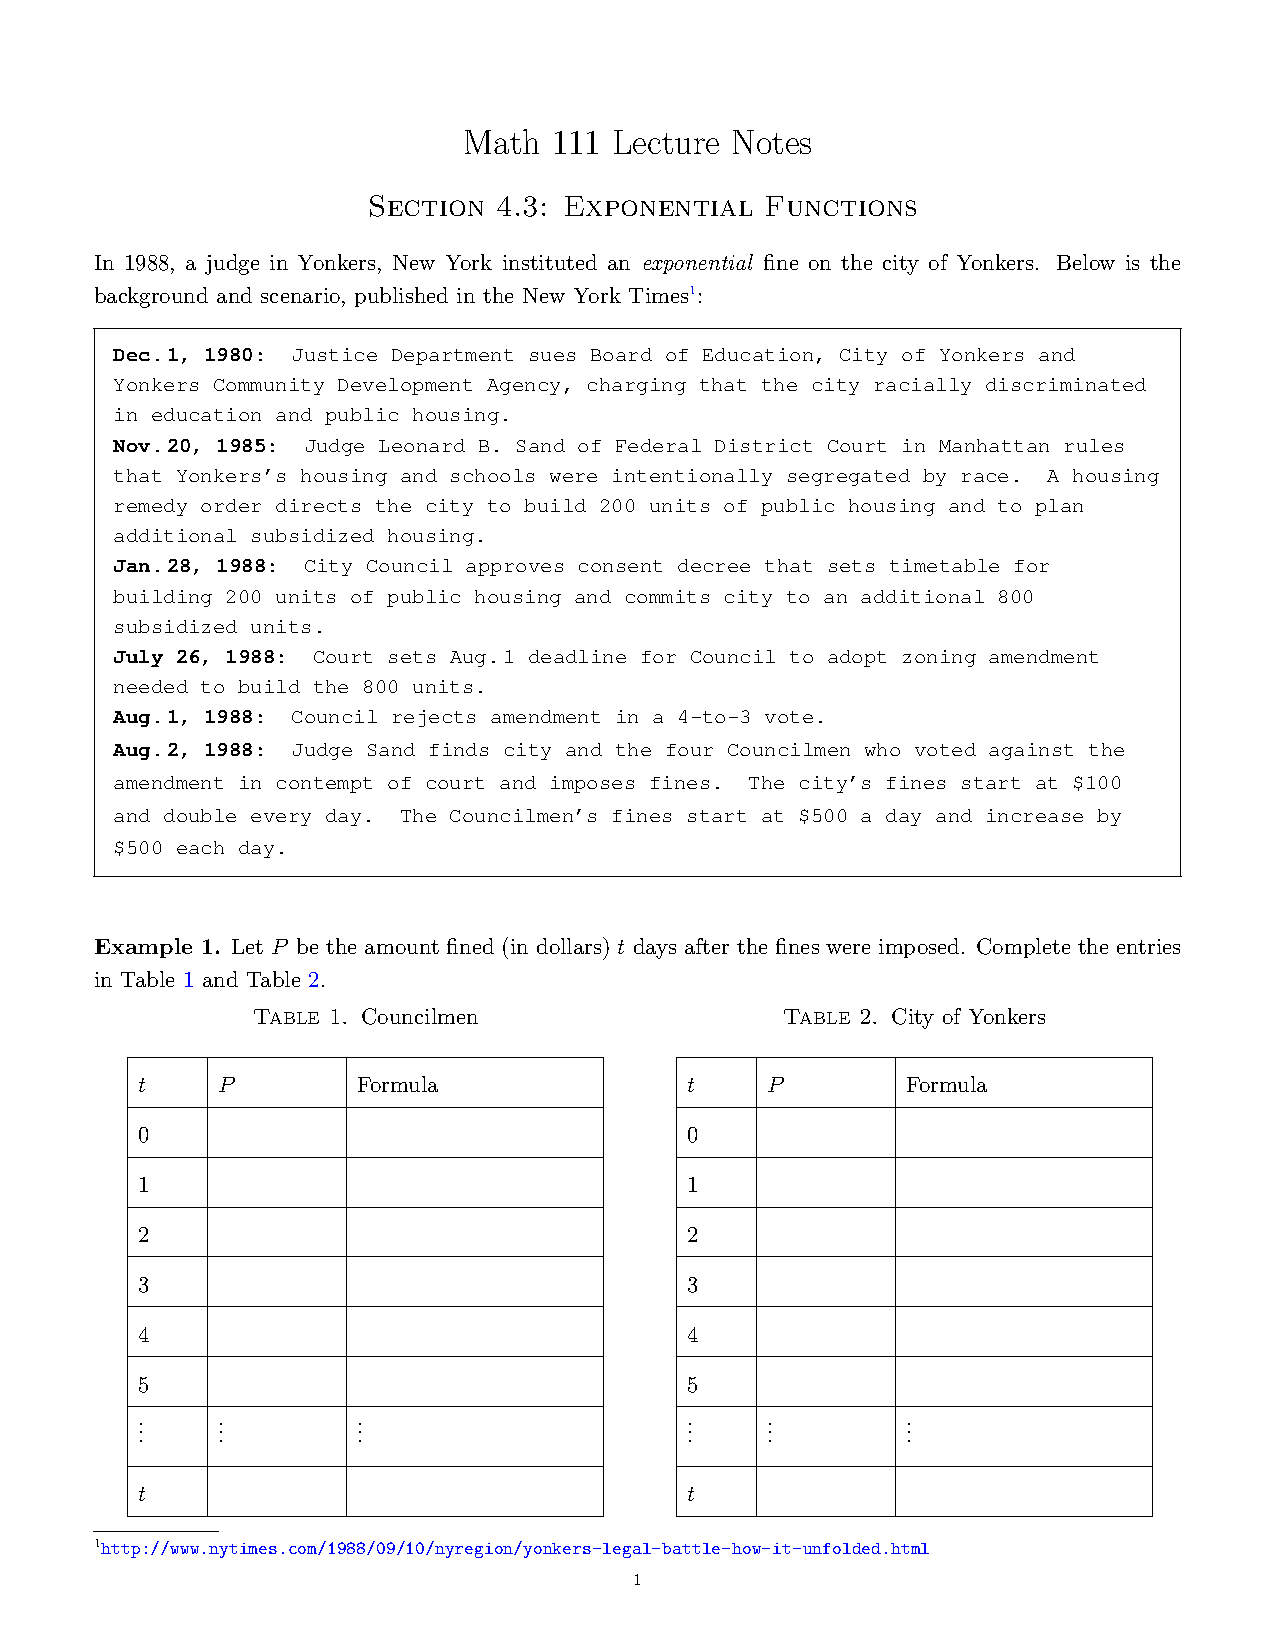
\includepdf[pages=-,pagecommand={\pagestyle{fancy}}]{./appendices/socialJusticeExample}

% arara: pdflatex: {files: [MathSACpr2014]}
% !arara: indent: {overwrite: yes}
\chapter{Class size report}\label{app:sec:classsize}
\emph{The report on the following pages was submitted to the DOIs}.

% http://tex.stackexchange.com/questions/117960/header-and-page-numbers-with-pdfpages
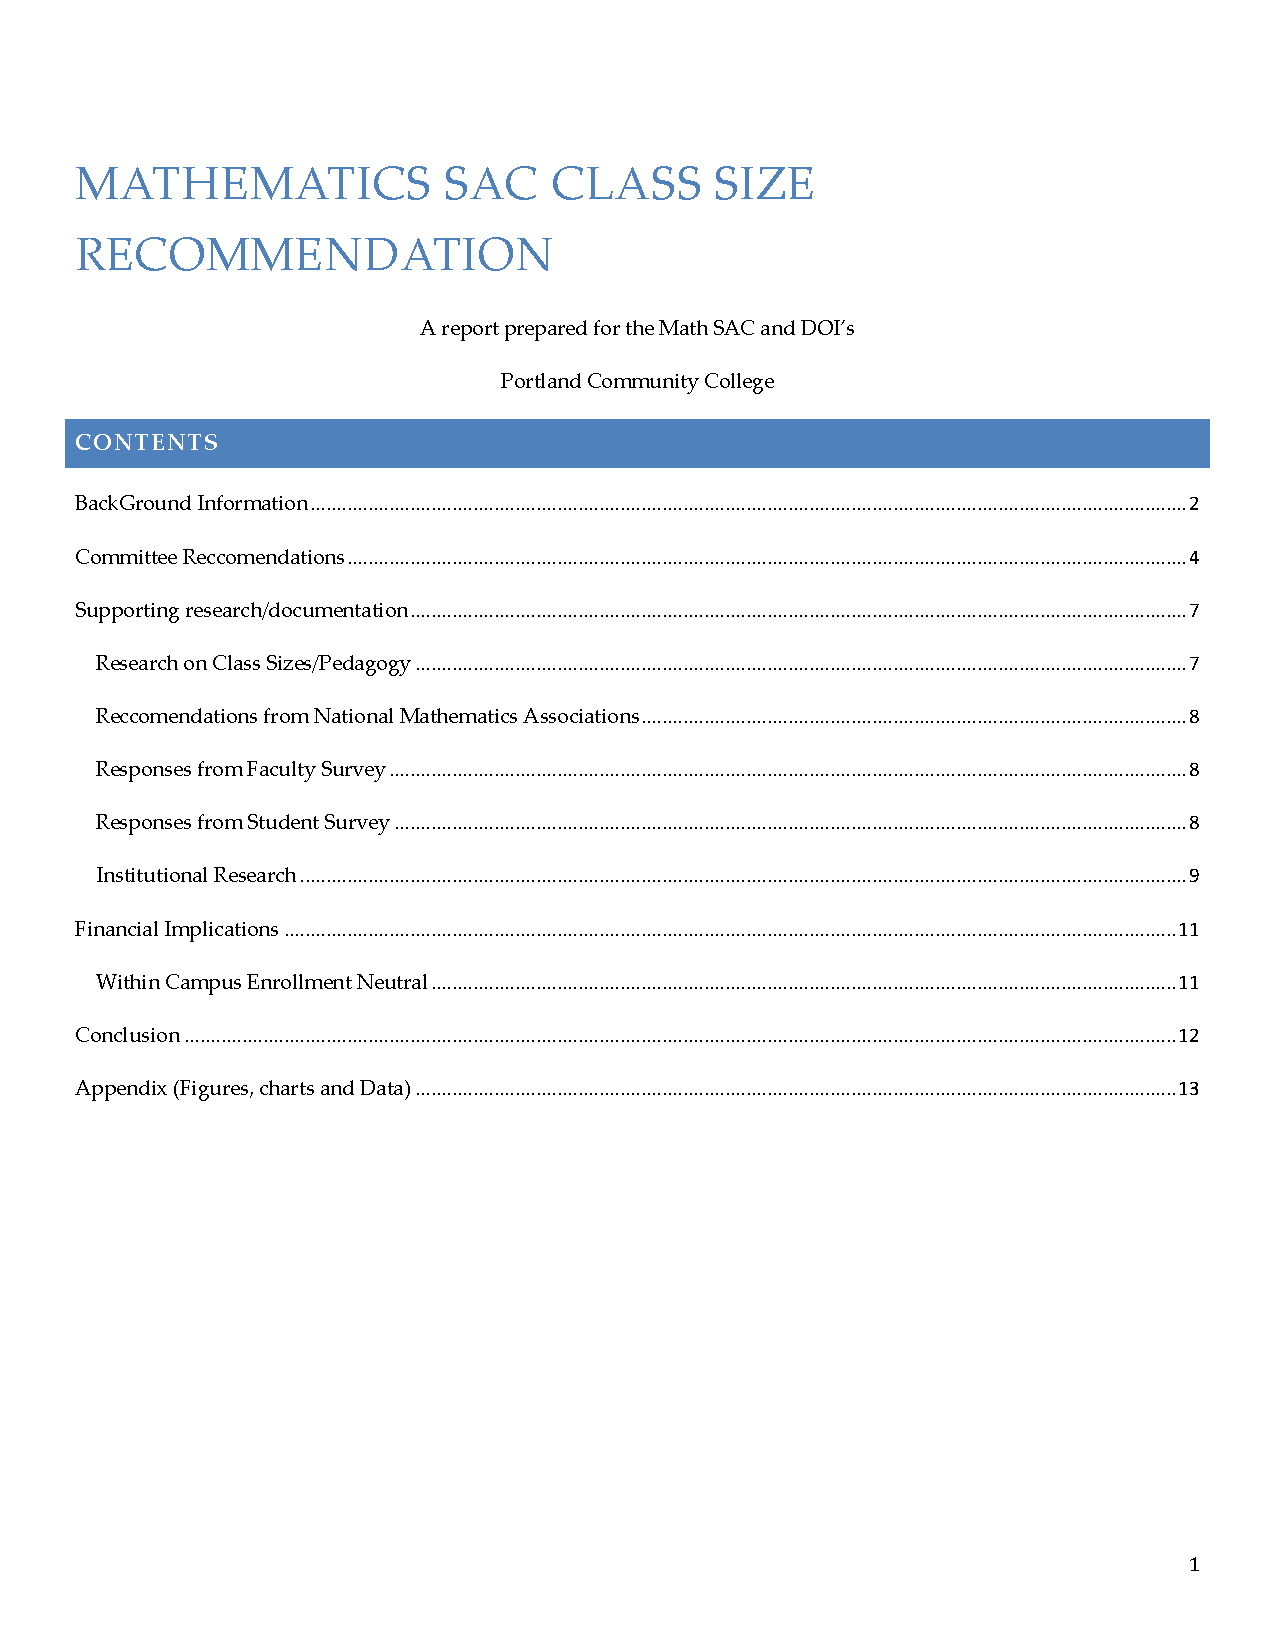
\includepdf[pages=-,pagecommand={\pagestyle{fancy}}]{appendices/classSizeRecommendations}

% arara: pdflatex: {files: [MathSACpr2014]}
% !arara: indent: {overwrite: yes}
\chapter{Demographic data}\label{app:sec:demographicdata}

\Crefrange{app:tab:demographic2008-2009}{app:tab:demographic2012-2013} show
demographic data for the academic years 2008 through 2013.

% the monster tables need bigger margins- don't worry, it
% is restored at the end
\newgeometry{left=0.5cm,right=0.5cm,
top=2cm,bottom=1.5cm,asymmetric=true,bindingoffset=0cm}
\begin{sidewaystable}
  \captionsetup{skip=0pt}
	\centering
	\caption{Demographic data for 2008--2009 (Pre-college level MTH and statistics)}
	% arara: pdflatex
\documentclass[varwidth]{standalone}
%\usepackage[landscape,textwidth=25cm]{geometry}
\usepackage{pgfplotstable}
\usepackage{booktabs}
\usepackage{multirow}

% caption: pass rates by demographic for 2008-2009
%           note that MTH 111 was split into MTH 111 A, B, C

% empty column type- very useful
\newcolumntype{H}{>{\setbox0=\hbox\bgroup}c<{\egroup}@{}}

\pgfplotstableset{percentstyle/.style={
    preproc/expr={##1*100},
    dec sep align,fixed,fixed zerofill,
postproc cell content/.append code={
            \ifx\\##1\\% check if ##1 is empty
            \else
            \ifnum1=\pgfplotstablepartno
                \pgfkeysalso{@cell content/.add={}{\,\%}}%
            \fi
            \fi
        },
    precision=0,
},
demographic/.style={},
}

% references:
%   http://tex.stackexchange.com/questions/65760/pgfplotstable-how-can-i-add-percent-signs-and-respect-dec-sep-align
%   http://tex.stackexchange.com/questions/16604/easiest-way-to-delete-a-column/16607#16607
%   http://tex.stackexchange.com/questions/89365/check-for-empty-macro-argument

\begin{document}

% http://tex.stackexchange.com/questions/128468/problems-with-pgfplotstableread-and-relative-paths
\IfStandalone{
	\newcommand{\fromRoot}[1]{../data/demographics/#1}
	}{
	\newcommand{\fromRoot}[1]{./data/demographics/#1}
}
\pgfplotstableread[col sep=comma]{\fromRoot{demographics2008-2009.csv}}\diversitydata

\noindent\resizebox{\textwidth}{!}{
\pgfplotstabletypeset[
every head row/.style={
        before row={%
        \toprule
        \multirow{2}{*}{2008--2009}
        & \multicolumn{7}{c}{MTH 20} 
        & \multicolumn{7}{c}{MTH 60} 
        & \multicolumn{7}{c}{MTH 65} 
        & \multicolumn{29}{c}{MTH 95} 
        & \multicolumn{10}{c}{MTH 243} 
        & \multicolumn{10}{c}{MTH 244} 
        \\},
        after row=\midrule},
every last row/.style={after row=\bottomrule},
every row no 3/.style={after row=\cmidrule{2-70}},
every row no 13/.style={after row=\cmidrule{2-70}},
demographic,
    columns/demographic/.style={string type,column name={},column type=l},
    % MTH 20 - ignore most of the columns
    columns/mth20p/.style={column type=H},
    columns/mth20np/.style={column type=H},
    columns/mth20tot/.style={column name=Total,column type=r},
    columns/mth20totper/.style={percentstyle,column name=\% Total},
    columns/mth20totpass/.style={percentstyle,column name=\% Pass},
    % MTH 60 - ignore most of the columns
    columns/mth60p/.style={column type=H},
    columns/mth60np/.style={column type=H},
    columns/mth60tot/.style={column name=Total,column type=r},
    columns/mth60totper/.style={percentstyle,column name=\% Total},
    columns/mth60totpass/.style={percentstyle,column name=\% Pass},
    % MTH 65 - ignore most of the columns
    columns/mth65p/.style={column type=H},
    columns/mth65np/.style={column type=H},
    columns/mth65tot/.style={column name=Total,column type=r},
    columns/mth65totper/.style={percentstyle,column name=\% Total},
    columns/mth65totpass/.style={percentstyle,column name=\% Pass},
    % MTH 95 - ignore most of the columns
    columns/mth95p/.style={column type=H},
    columns/mth95np/.style={column type=H},
    columns/mth95tot/.style={column name=Total,column type=r},
    columns/mth95totper/.style={percentstyle,column name=\% Total},
    columns/mth95totpass/.style={percentstyle,column name=\% Pass},
    % MTH 111A - ignore all of the columns
    columns/mth111Ap/.style={column type=H},
    columns/mth111Anp/.style={column type=H},
    columns/mth111Atot/.style={column type=H},
    columns/mth111Atotper/.style={column type=H},
    columns/mth111Atotpass/.style={column type=H},
    % MTH 111B - ignore all of the columns
    columns/mth111Bp/.style={column type=H},
    columns/mth111Bnp/.style={column type=H},
    columns/mth111Btot/.style={column type=H},
    columns/mth111Btotper/.style={column type=H},
    columns/mth111Btotpass/.style={column type=H},
    % MTH 111C - ignore all of the columns
    columns/mth111Cp/.style={column type=H},
    columns/mth111Cnp/.style={column type=H},
    columns/mth111Ctot/.style={column type=H},
    columns/mth111Ctotper/.style={column type=H},
    columns/mth111Ctotpass/.style={column type=H},
    % MTH 111BC - ignore most of the columns
    columns/mth111BCp/.style={column type=H},
    columns/mth111BCnp/.style={column type=H},
    columns/mth111BCtot/.style={column type=H},
    columns/mth111BCtotper/.style={column type=H},
    columns/mth111BCtotpass/.style={column type=H},
    % MTH 112 - ignore most of the columns
    columns/mth112p/.style={column type=H},
    columns/mth112np/.style={column type=H},
    columns/mth112tot/.style={column type=H},
    columns/mth112totper/.style={column type=H},
    columns/mth112totpass/.style={column type=H},
    % MTH 243 - ignore most of the columns
    columns/mth243p/.style={column type=H},
    columns/mth243np/.style={column type=H},
    columns/mth243tot/.style={column name=Total,column type=r},
    columns/mth243totper/.style={percentstyle,column name=\% Total},
    columns/mth243totpass/.style={percentstyle,column name=\% Pass},
    % MTH 244 - ignore most of the columns
    columns/mth244p/.style={column type=H},
    columns/mth244np/.style={column type=H},
    columns/mth244tot/.style={column name=Total,column type=r},
    columns/mth244totper/.style={percentstyle,column name=\% Total},
    columns/mth244totpass/.style={percentstyle,column name=\% Pass},
    % MTH 251 - ignore most of the columns
    columns/mth251p/.style={column type=H},
    columns/mth251np/.style={column type=H},
    columns/mth251tot/.style={column type=H},
    columns/mth251totper/.style={column type=H},
    columns/mth251totpass/.style={column type=H},
    % MTH 252 - ignore most of the columns
    columns/mth252p/.style={column type=H},
    columns/mth252np/.style={column type=H},
    columns/mth252tot/.style={column type=H},
    columns/mth252totper/.style={column type=H},
    columns/mth252totpass/.style={column type=H},
    % MTH 253 - ignore most of the columns
    columns/mth253p/.style={column type=H},
    columns/mth253np/.style={column type=H},
    columns/mth253tot/.style={column type=H},
    columns/mth253totper/.style={column type=H},
    columns/mth253totpass/.style={column type=H},
    % MTH 254 - ignore most of the columns
    columns/mth254p/.style={column type=H},
    columns/mth254np/.style={column type=H},
    columns/mth254tot/.style={column type=H},
    columns/mth254totper/.style={column type=H},
    columns/mth254totpass/.style={column type=H},
]{\diversitydata}
}

\end{document}

	\caption{Demographic data for 2008--2009 (College level MTH)}
	% arara: pdflatex
\documentclass[varwidth]{standalone}
%\usepackage[landscape,textwidth=25cm]{geometry}
\usepackage{pgfplotstable}
\usepackage{booktabs}
\usepackage{multirow}

% caption: pass rates by demographic for 2008-2009
%           note that MTH 111 was split into MTH 111 A, B, C

% empty column type- very useful
\newcolumntype{H}{>{\setbox0=\hbox\bgroup}c<{\egroup}@{}}

\pgfplotstableset{percentstyle/.style={
    preproc/expr={##1*100},
    dec sep align,fixed,fixed zerofill,
postproc cell content/.append code={
            \ifx\\##1\\% check if ##1 is empty
            \else
            \ifnum1=\pgfplotstablepartno
                \pgfkeysalso{@cell content/.add={}{\,\%}}%
            \fi
            \fi
        },
    precision=0,
}
}

% references:
%   http://tex.stackexchange.com/questions/65760/pgfplotstable-how-can-i-add-percent-signs-and-respect-dec-sep-align
%   http://tex.stackexchange.com/questions/16604/easiest-way-to-delete-a-column/16607#16607
%   http://tex.stackexchange.com/questions/89365/check-for-empty-macro-argument

\begin{document}

% http://tex.stackexchange.com/questions/128468/problems-with-pgfplotstableread-and-relative-paths
\IfStandalone{
	\newcommand{\fromRoot}[1]{../data/demographics/#1}
	}{
	\newcommand{\fromRoot}[1]{./data/demographics/#1}
}
\pgfplotstableread[col sep=comma]{\fromRoot{demographics2008-2009.csv}}\diversitydata

\noindent\resizebox{\textwidth}{!}{
\pgfplotstabletypeset[
every head row/.style={
        before row={%
        \toprule
        \multirow{2}{*}{2008--2009}
        & \multicolumn{30}{c}{MTH 111A} 
        & \multicolumn{15}{c}{MTH 111 B\&C} 
        & \multicolumn{11}{c}{MTH 112} 
        & \multicolumn{12}{c}{MTH 251} 
        & \multicolumn{7}{c}{MTH 252} 
        & \multicolumn{7}{c}{MTH 253} 
        & \multicolumn{7}{c}{MTH 254}\\},
        after row=\midrule},
every last row/.style={after row=\bottomrule},
every row no 3/.style={after row=\cmidrule{2-90}},
every row no 13/.style={after row=\cmidrule{2-90}},
    columns/demographic/.style={string type,column name={},column type=l},
    % MTH 20 - ignore most of the columns
    columns/mth20p/.style={column type=H},
    columns/mth20np/.style={column type=H},
    columns/mth20tot/.style={column type=H},
    columns/mth20totper/.style={column type=H},
    columns/mth20totpass/.style={column type=H},
    % MTH 60 - ignore most of the columns
    columns/mth60p/.style={column type=H},
    columns/mth60np/.style={column type=H},
    columns/mth60tot/.style={column type=H},
    columns/mth60totper/.style={column type=H},
    columns/mth60totpass/.style={column type=H},
    % MTH 65 - ignore most of the columns
    columns/mth65p/.style={column type=H},
    columns/mth65np/.style={column type=H},
    columns/mth65tot/.style={column type=H},
    columns/mth65totper/.style={column type=H},
    columns/mth65totpass/.style={column type=H},
    % MTH 95 - ignore most of the columns
    columns/mth95p/.style={column type=H},
    columns/mth95np/.style={column type=H},
    columns/mth95tot/.style={column type=H},
    columns/mth95totper/.style={column type=H},
    columns/mth95totpass/.style={column type=H},
    % MTH 111A - ignore all of the columns
    columns/mth111Ap/.style={column type=H},
    columns/mth111Anp/.style={column type=H},
    columns/mth111Atot/.style={column name=Total,column type=r},
    columns/mth111Atotper/.style={percentstyle,column name=\% Total},
    columns/mth111Atotpass/.style={percentstyle,column name=\% Pass},
    % MTH 111B - ignore all of the columns
    columns/mth111Bp/.style={column type=H},
    columns/mth111Bnp/.style={column type=H},
    columns/mth111Btot/.style={column type=H},
    columns/mth111Btotper/.style={column type=H},
    columns/mth111Btotpass/.style={column type=H},
    % MTH 111C - ignore all of the columns
    columns/mth111Cp/.style={column type=H},
    columns/mth111Cnp/.style={column type=H},
    columns/mth111Ctot/.style={column type=H},
    columns/mth111Ctotper/.style={column type=H},
    columns/mth111Ctotpass/.style={column type=H},
    % MTH 111BC - ignore most of the columns
    columns/mth111BCp/.style={column type=H},
    columns/mth111BCnp/.style={column type=H},
    columns/mth111BCtot/.style={column name=Total,column type=r},
    columns/mth111BCtotper/.style={percentstyle,column name=\% Total},
    columns/mth111BCtotpass/.style={percentstyle,column name=\% Pass},
    % MTH 112 - ignore most of the columns
    columns/mth112p/.style={column type=H},
    columns/mth112np/.style={column type=H},
    columns/mth112tot/.style={column name=Total,column type=r},
    columns/mth112totper/.style={percentstyle,column name=\% Total},
    columns/mth112totpass/.style={percentstyle,column name=\% Pass},
    % MTH 243 - ignore most of the columns
    columns/mth243p/.style={column type=H},
    columns/mth243np/.style={column type=H},
    columns/mth243tot/.style={column type=H},
    columns/mth243totper/.style={column type=H},
    columns/mth243totpass/.style={column type=H},
    % MTH 244 - ignore most of the columns
    columns/mth244p/.style={column type=H},
    columns/mth244np/.style={column type=H},
    columns/mth244tot/.style={column type=H},
    columns/mth244totper/.style={column type=H},
    columns/mth244totpass/.style={column type=H},
    % MTH 251 - ignore most of the columns
    columns/mth251p/.style={column type=H},
    columns/mth251np/.style={column type=H},
    columns/mth251tot/.style={column name=Total,column type=r},
    columns/mth251totper/.style={percentstyle,column name=\% Total},
    columns/mth251totpass/.style={percentstyle,column name=\% Pass},
    % MTH 252 - ignore most of the columns
    columns/mth252p/.style={column type=H},
    columns/mth252np/.style={column type=H},
    columns/mth252tot/.style={column name=Total,column type=r},
    columns/mth252totper/.style={percentstyle,column name=\% Total},
    columns/mth252totpass/.style={percentstyle,column name=\% Pass},
    % MTH 253 - ignore most of the columns
    columns/mth253p/.style={column type=H},
    columns/mth253np/.style={column type=H},
    columns/mth253tot/.style={column name=Total,column type=r},
    columns/mth253totper/.style={percentstyle,column name=\% Total},
    columns/mth253totpass/.style={percentstyle,column name=\% Pass},
    % MTH 254 - ignore most of the columns
    columns/mth254p/.style={column type=H},
    columns/mth254np/.style={column type=H},
    columns/mth254tot/.style={column name=Total,column type=r},
    columns/mth254totper/.style={percentstyle,column name=\% Total},
    columns/mth254totpass/.style={percentstyle,column name=\% Pass},
]{\diversitydata}
}

\end{document}

\end{sidewaystable}
\begin{sidewaystable}
  \captionsetup{skip=0pt}
	\centering
	\caption{Demographic data for 2009--2010 (Pre-college level MTH and statistics)}
	% arara: pdflatex
\documentclass[varwidth]{standalone}
%\usepackage[landscape,textwidth=25cm]{geometry}
\usepackage{pgfplotstable}
\usepackage{booktabs}
\usepackage{multirow}

% caption: pass rates by demographic for 2009-2010
%           note that MTH 111 was split into MTH 111 A, B, C
%           and that there was 0 enrollment in MTH 111A which is
%           why it is not displayed.

% empty column type- very useful
\newcolumntype{H}{>{\setbox0=\hbox\bgroup}c<{\egroup}@{}}

\pgfplotstableset{percentstyle/.style={
    preproc/expr={##1*100},
    dec sep align,fixed,fixed zerofill,
postproc cell content/.append code={
            \ifx\\##1\\% check if ##1 is empty
            \else
            \ifnum1=\pgfplotstablepartno
                \pgfkeysalso{@cell content/.add={}{\,\%}}%
            \fi
            \fi
        },
    precision=0,
}
}

% references:
%   http://tex.stackexchange.com/questions/65760/pgfplotstable-how-can-i-add-percent-signs-and-respect-dec-sep-align
%   http://tex.stackexchange.com/questions/16604/easiest-way-to-delete-a-column/16607#16607
%   http://tex.stackexchange.com/questions/89365/check-for-empty-macro-argument

\begin{document}

% http://tex.stackexchange.com/questions/128468/problems-with-pgfplotstableread-and-relative-paths
\IfStandalone{
	\newcommand{\fromRoot}[1]{../data/demographics/#1}
	}{
	\newcommand{\fromRoot}[1]{./data/demographics/#1}
}

\pgfplotstableread[col sep=comma]{\fromRoot{demographics2009-2010.csv}}\diversitydata

%Note that MTH 111A had $0$ enrollment for 2009--2010, so its data is not displayed.

\noindent\resizebox{\textwidth}{!}{
\pgfplotstabletypeset[
every head row/.style={
        before row={%
        \toprule
        \multirow{2}{*}{2009--2010}
        & \multicolumn{7}{c}{MTH 20} 
        & \multicolumn{7}{c}{MTH 60} 
        & \multicolumn{7}{c}{MTH 65} 
        & \multicolumn{29}{c}{MTH 95} 
        & \multicolumn{10}{c}{MTH 243} 
        & \multicolumn{10}{c}{MTH 244} 
        \\},
        after row=\midrule},
every last row/.style={after row=\bottomrule},
every row no 3/.style={after row=\cmidrule{2-80}},
every row no 13/.style={after row=\cmidrule{2-80}},
    columns/demographic/.style={string type,column name={},column type=l},
    % MTH 20 - ignore most of the columns
    columns/mth20p/.style={column type=H},
    columns/mth20np/.style={column type=H},
    columns/mth20tot/.style={column name=Total,column type=r},
    columns/mth20totper/.style={percentstyle,column name=\% Total},
    columns/mth20totpass/.style={percentstyle,column name=\% Pass},
    % MTH 60 - ignore most of the columns
    columns/mth60p/.style={column type=H},
    columns/mth60np/.style={column type=H},
    columns/mth60tot/.style={column name=Total,column type=r},
    columns/mth60totper/.style={percentstyle,column name=\% Total},
    columns/mth60totpass/.style={percentstyle,column name=\% Pass},
    % MTH 65 - ignore most of the columns
    columns/mth65p/.style={column type=H},
    columns/mth65np/.style={column type=H},
    columns/mth65tot/.style={column name=Total,column type=r},
    columns/mth65totper/.style={percentstyle,column name=\% Total},
    columns/mth65totpass/.style={percentstyle,column name=\% Pass},
    % MTH 95 - ignore most of the columns
    columns/mth95p/.style={column type=H},
    columns/mth95np/.style={column type=H},
    columns/mth95tot/.style={column name=Total,column type=r},
    columns/mth95totper/.style={percentstyle,column name=\% Total},
    columns/mth95totpass/.style={percentstyle,column name=\% Pass},
    % MTH 111A - ignore all of the columns
    columns/mth111Ap/.style={column type=H},
    columns/mth111Anp/.style={column type=H},
    columns/mth111Atot/.style={column type=H},
    columns/mth111Atotper/.style={column type=H},
    columns/mth111Atotpass/.style={column type=H},
    % MTH 111B - ignore all of the columns
    columns/mth111Bp/.style={column type=H},
    columns/mth111Bnp/.style={column type=H},
    columns/mth111Btot/.style={column type=H},
    columns/mth111Btotper/.style={column type=H},
    columns/mth111Btotpass/.style={column type=H},
    % MTH 111C - ignore all of the columns
    columns/mth111Cp/.style={column type=H},
    columns/mth111Cnp/.style={column type=H},
    columns/mth111Ctot/.style={column type=H},
    columns/mth111Ctotper/.style={column type=H},
    columns/mth111Ctotpass/.style={column type=H},
    % MTH 111BC - ignore most of the columns
    columns/mth111BCp/.style={column type=H},
    columns/mth111BCnp/.style={column type=H},
    columns/mth111BCtot/.style={column type=H},
    columns/mth111BCtotper/.style={column type=H},
    columns/mth111BCtotpass/.style={column type=H},
    % MTH 112 - ignore most of the columns
    columns/mth112p/.style={column type=H},
    columns/mth112np/.style={column type=H},
    columns/mth112tot/.style={column type=H},
    columns/mth112totper/.style={column type=H},
    columns/mth112totpass/.style={column type=H},
    % MTH 243 - ignore most of the columns
    columns/mth243p/.style={column type=H},
    columns/mth243np/.style={column type=H},
    columns/mth243tot/.style={column name=Total,column type=r},
    columns/mth243totper/.style={percentstyle,column name=\% Total},
    columns/mth243totpass/.style={percentstyle,column name=\% Pass},
    % MTH 244 - ignore most of the columns
    columns/mth244p/.style={column type=H},
    columns/mth244np/.style={column type=H},
    columns/mth244tot/.style={column name=Total,column type=r},
    columns/mth244totper/.style={percentstyle,column name=\% Total},
    columns/mth244totpass/.style={percentstyle,column name=\% Pass},
    % MTH 251 - ignore most of the columns
    columns/mth251p/.style={column type=H},
    columns/mth251np/.style={column type=H},
    columns/mth251tot/.style={column type=H},
    columns/mth251totper/.style={column type=H},
    columns/mth251totpass/.style={column type=H},
    % MTH 252 - ignore most of the columns
    columns/mth252p/.style={column type=H},
    columns/mth252np/.style={column type=H},
    columns/mth252tot/.style={column type=H},
    columns/mth252totper/.style={column type=H},
    columns/mth252totpass/.style={column type=H},
    % MTH 253 - ignore most of the columns
    columns/mth253p/.style={column type=H},
    columns/mth253np/.style={column type=H},
    columns/mth253tot/.style={column type=H},
    columns/mth253totper/.style={column type=H},
    columns/mth253totpass/.style={column type=H},
    % MTH 254 - ignore most of the columns
    columns/mth254p/.style={column type=H},
    columns/mth254np/.style={column type=H},
    columns/mth254tot/.style={column type=H},
    columns/mth254totper/.style={column type=H},
    columns/mth254totpass/.style={column type=H},
]{\diversitydata}
}

\end{document}

	\caption{Demographic data for 2009--2010 (College level MTH). Note that MTH 111A had $0$ enrollment for 2009--2010, so its data is not displayed. }
	% arara: pdflatex
\documentclass[varwidth]{standalone}
%\usepackage[landscape,textwidth=25cm]{geometry}
\usepackage{pgfplotstable}
\usepackage{booktabs}
\usepackage{multirow}

% caption: pass rates by demographic for 2009-2010
%           note that MTH 111 was split into MTH 111 A, B, C
%           and that there was 0 enrollment in MTH 111A which is
%           why it is not displayed.

% empty column type- very useful
\newcolumntype{H}{>{\setbox0=\hbox\bgroup}c<{\egroup}@{}}

\pgfplotstableset{percentstyle/.style={
    preproc/expr={##1*100},
    dec sep align,fixed,fixed zerofill,
postproc cell content/.append code={
            \ifx\\##1\\% check if ##1 is empty
            \else
            \ifnum1=\pgfplotstablepartno
                \pgfkeysalso{@cell content/.add={}{\,\%}}%
            \fi
            \fi
        },
    precision=0,
}
}

% references:
%   http://tex.stackexchange.com/questions/65760/pgfplotstable-how-can-i-add-percent-signs-and-respect-dec-sep-align
%   http://tex.stackexchange.com/questions/16604/easiest-way-to-delete-a-column/16607#16607
%   http://tex.stackexchange.com/questions/89365/check-for-empty-macro-argument

\begin{document}

% http://tex.stackexchange.com/questions/128468/problems-with-pgfplotstableread-and-relative-paths
\IfStandalone{
	\newcommand{\fromRoot}[1]{../data/demographics/#1}
	}{
	\newcommand{\fromRoot}[1]{./data/demographics/#1}
}

\pgfplotstableread[col sep=comma]{\fromRoot{demographics2009-2010.csv}}\diversitydata

%Note that MTH 111A had $0$ enrollment for 2009--2010, so its data is not displayed.

\noindent\resizebox{\textwidth}{!}{
\pgfplotstabletypeset[
every head row/.style={
        before row={%
        \toprule
        \multirow{2}{*}{2009--2010}
        & \multicolumn{44}{c}{MTH 111 B\&C}
        & \multicolumn{5}{c}{MTH 112} 
        & \multicolumn{17}{c}{MTH 251} 
        & \multicolumn{7}{c}{MTH 252} 
        & \multicolumn{7}{c}{MTH 253} 
        & \multicolumn{7}{c}{MTH 254}\\},
        after row=\midrule},
every last row/.style={after row=\bottomrule},
every row no 3/.style={after row=\cmidrule{2-80}},
every row no 13/.style={after row=\cmidrule{2-80}},
    columns/demographic/.style={string type,column name={},column type=l},
    % MTH 20 - ignore most of the columns
    columns/mth20p/.style={column type=H},
    columns/mth20np/.style={column type=H},
    columns/mth20tot/.style={column type=H},
    columns/mth20totper/.style={column type=H},
    columns/mth20totpass/.style={column type=H},
    % MTH 60 - ignore most of the columns
    columns/mth60p/.style={column type=H},
    columns/mth60np/.style={column type=H},
    columns/mth60tot/.style={column type=H},
    columns/mth60totper/.style={column type=H},
    columns/mth60totpass/.style={column type=H},
    % MTH 65 - ignore most of the columns
    columns/mth65p/.style={column type=H},
    columns/mth65np/.style={column type=H},
    columns/mth65tot/.style={column type=H},
    columns/mth65totper/.style={column type=H},
    columns/mth65totpass/.style={column type=H},
    % MTH 95 - ignore most of the columns
    columns/mth95p/.style={column type=H},
    columns/mth95np/.style={column type=H},
    columns/mth95tot/.style={column type=H},
    columns/mth95totper/.style={column type=H},
    columns/mth95totpass/.style={column type=H},
    % MTH 111A - ignore all of the columns
    columns/mth111Ap/.style={column type=H},
    columns/mth111Anp/.style={column type=H},
    columns/mth111Atot/.style={column type=H},
    columns/mth111Atotper/.style={column type=H},
    columns/mth111Atotpass/.style={column type=H},
    % MTH 111B - ignore all of the columns
    columns/mth111Bp/.style={column type=H},
    columns/mth111Bnp/.style={column type=H},
    columns/mth111Btot/.style={column type=H},
    columns/mth111Btotper/.style={column type=H},
    columns/mth111Btotpass/.style={column type=H},
    % MTH 111C - ignore all of the columns
    columns/mth111Cp/.style={column type=H},
    columns/mth111Cnp/.style={column type=H},
    columns/mth111Ctot/.style={column type=H},
    columns/mth111Ctotper/.style={column type=H},
    columns/mth111Ctotpass/.style={column type=H},
    % MTH 111BC - ignore most of the columns
    columns/mth111BCp/.style={column type=H},
    columns/mth111BCnp/.style={column type=H},
    columns/mth111BCtot/.style={column name=Total,column type=r},
    columns/mth111BCtotper/.style={percentstyle,column name=\% Total},
    columns/mth111BCtotpass/.style={percentstyle,column name=\% Pass},
    % MTH 112 - ignore most of the columns
    columns/mth112p/.style={column type=H},
    columns/mth112np/.style={column type=H},
    columns/mth112tot/.style={column name=Total,column type=r},
    columns/mth112totper/.style={percentstyle,column name=\% Total},
    columns/mth112totpass/.style={percentstyle,column name=\% Pass},
    % MTH 243 - ignore most of the columns
    columns/mth243p/.style={column type=H},
    columns/mth243np/.style={column type=H},
    columns/mth243tot/.style={column type=H},
    columns/mth243totper/.style={column type=H},
    columns/mth243totpass/.style={column type=H},
    % MTH 244 - ignore most of the columns
    columns/mth244p/.style={column type=H},
    columns/mth244np/.style={column type=H},
    columns/mth244tot/.style={column type=H},
    columns/mth244totper/.style={column type=H},
    columns/mth244totpass/.style={column type=H},
    % MTH 251 - ignore most of the columns
    columns/mth251p/.style={column type=H},
    columns/mth251np/.style={column type=H},
    columns/mth251tot/.style={column name=Total,column type=r},
    columns/mth251totper/.style={percentstyle,column name=\% Total},
    columns/mth251totpass/.style={percentstyle,column name=\% Pass},
    % MTH 252 - ignore most of the columns
    columns/mth252p/.style={column type=H},
    columns/mth252np/.style={column type=H},
    columns/mth252tot/.style={column name=Total,column type=r},
    columns/mth252totper/.style={percentstyle,column name=\% Total},
    columns/mth252totpass/.style={percentstyle,column name=\% Pass},
    % MTH 253 - ignore most of the columns
    columns/mth253p/.style={column type=H},
    columns/mth253np/.style={column type=H},
    columns/mth253tot/.style={column name=Total,column type=r},
    columns/mth253totper/.style={percentstyle,column name=\% Total},
    columns/mth253totpass/.style={percentstyle,column name=\% Pass},
    % MTH 254 - ignore most of the columns
    columns/mth254p/.style={column type=H},
    columns/mth254np/.style={column type=H},
    columns/mth254tot/.style={column name=Total,column type=r},
    columns/mth254totper/.style={percentstyle,column name=\% Total},
    columns/mth254totpass/.style={percentstyle,column name=\% Pass},
]{\diversitydata}
}

\end{document}

\end{sidewaystable}
\begin{sidewaystable}
  \captionsetup{skip=0pt}
	\centering
	\caption{Demographic data for 2010--2011 (Pre-college level MTH and statistics)}
	% arara: pdflatex
\documentclass[varwidth]{standalone}
%\usepackage[landscape,textwidth=25cm]{geometry}
\usepackage{pgfplotstable}
\usepackage{booktabs}
\usepackage{multirow}

% caption: pass rates by demographic for 2010-2011
%           note that MTH 111 was split into MTH 111 A, B, C
%           and that there was 0 enrollment in MTH 111A which is
%           why it is not displayed.

% empty column type- very useful
\newcolumntype{H}{>{\setbox0=\hbox\bgroup}c<{\egroup}@{}}

\pgfplotstableset{percentstyle/.style={
    preproc/expr={##1*100},
    dec sep align,fixed,fixed zerofill,
postproc cell content/.append code={
            \ifx\\##1\\% check if ##1 is empty
            \else
            \ifnum1=\pgfplotstablepartno
                \pgfkeysalso{@cell content/.add={}{\,\%}}%
            \fi
            \fi
        },
    precision=0,
}
}

% references:
%   http://tex.stackexchange.com/questions/65760/pgfplotstable-how-can-i-add-percent-signs-and-respect-dec-sep-align
%   http://tex.stackexchange.com/questions/16604/easiest-way-to-delete-a-column/16607#16607
%   http://tex.stackexchange.com/questions/89365/check-for-empty-macro-argument

\begin{document}

% http://tex.stackexchange.com/questions/128468/problems-with-pgfplotstableread-and-relative-paths
\IfStandalone{
	\newcommand{\fromRoot}[1]{../data/demographics/#1}
	}{
	\newcommand{\fromRoot}[1]{./data/demographics/#1}
}
\pgfplotstableread[col sep=comma]{\fromRoot{demographics2010-2011.csv}}\diversitydata

%Note that MTH 111A had $0$ enrollment for 2010--2011, so its data is not displayed.

\noindent\resizebox{\textwidth}{!}{
\pgfplotstabletypeset[
every head row/.style={
        before row={%
        \toprule
        \multirow{2}{*}{2010--2011}
        & \multicolumn{7}{c}{MTH 20} 
        & \multicolumn{7}{c}{MTH 60} 
        & \multicolumn{7}{c}{MTH 65} 
        & \multicolumn{29}{c}{MTH 95} 
        & \multicolumn{10}{c}{MTH 243} 
        & \multicolumn{10}{c}{MTH 244} 
        \\},
        after row=\midrule},
every last row/.style={after row=\bottomrule},
every row no 3/.style={after row=\cmidrule{2-80}},
every row no 13/.style={after row=\cmidrule{2-80}},
    columns/demographic/.style={string type,column name={},column type=l},
    % MTH 20 - ignore most of the columns
    columns/mth20p/.style={column type=H},
    columns/mth20np/.style={column type=H},
    columns/mth20tot/.style={column name=Total,column type=r},
    columns/mth20totper/.style={percentstyle,column name=\% Total},
    columns/mth20totpass/.style={percentstyle,column name=\% Pass},
    % MTH 60 - ignore most of the columns
    columns/mth60p/.style={column type=H},
    columns/mth60np/.style={column type=H},
    columns/mth60tot/.style={column name=Total,column type=r},
    columns/mth60totper/.style={percentstyle,column name=\% Total},
    columns/mth60totpass/.style={percentstyle,column name=\% Pass},
    % MTH 65 - ignore most of the columns
    columns/mth65p/.style={column type=H},
    columns/mth65np/.style={column type=H},
    columns/mth65tot/.style={column name=Total,column type=r},
    columns/mth65totper/.style={percentstyle,column name=\% Total},
    columns/mth65totpass/.style={percentstyle,column name=\% Pass},
    % MTH 95 - ignore most of the columns
    columns/mth95p/.style={column type=H},
    columns/mth95np/.style={column type=H},
    columns/mth95tot/.style={column name=Total,column type=r},
    columns/mth95totper/.style={percentstyle,column name=\% Total},
    columns/mth95totpass/.style={percentstyle,column name=\% Pass},
    % MTH 111A - ignore all of the columns
    columns/mth111Ap/.style={column type=H},
    columns/mth111Anp/.style={column type=H},
    columns/mth111Atot/.style={column type=H},
    columns/mth111Atotper/.style={column type=H},
    columns/mth111Atotpass/.style={column type=H},
    % MTH 111B - ignore all of the columns
    columns/mth111Bp/.style={column type=H},
    columns/mth111Bnp/.style={column type=H},
    columns/mth111Btot/.style={column type=H},
    columns/mth111Btotper/.style={column type=H},
    columns/mth111Btotpass/.style={column type=H},
    % MTH 111C - ignore all of the columns
    columns/mth111Cp/.style={column type=H},
    columns/mth111Cnp/.style={column type=H},
    columns/mth111Ctot/.style={column type=H},
    columns/mth111Ctotper/.style={column type=H},
    columns/mth111Ctotpass/.style={column type=H},
    % MTH 111BC - ignore most of the columns
    columns/mth111BCp/.style={column type=H},
    columns/mth111BCnp/.style={column type=H},
    columns/mth111BCtot/.style={column type=H},
    columns/mth111BCtotper/.style={column type=H},
    columns/mth111BCtotpass/.style={column type=H},
    % MTH 112 - ignore most of the columns
    columns/mth112p/.style={column type=H},
    columns/mth112np/.style={column type=H},
    columns/mth112tot/.style={column type=H},
    columns/mth112totper/.style={column type=H},
    columns/mth112totpass/.style={column type=H},
    % MTH 243 - ignore most of the columns
    columns/mth243p/.style={column type=H},
    columns/mth243np/.style={column type=H},
    columns/mth243tot/.style={column name=Total,column type=r},
    columns/mth243totper/.style={percentstyle,column name=\% Total},
    columns/mth243totpass/.style={percentstyle,column name=\% Pass},
    % MTH 244 - ignore most of the columns
    columns/mth244p/.style={column type=H},
    columns/mth244np/.style={column type=H},
    columns/mth244tot/.style={column name=Total,column type=r},
    columns/mth244totper/.style={percentstyle,column name=\% Total},
    columns/mth244totpass/.style={percentstyle,column name=\% Pass},
    % MTH 251 - ignore most of the columns
    columns/mth251p/.style={column type=H},
    columns/mth251np/.style={column type=H},
    columns/mth251tot/.style={column type=H},
    columns/mth251totper/.style={column type=H},
    columns/mth251totpass/.style={column type=H},
    % MTH 252 - ignore most of the columns
    columns/mth252p/.style={column type=H},
    columns/mth252np/.style={column type=H},
    columns/mth252tot/.style={column type=H},
    columns/mth252totper/.style={column type=H},
    columns/mth252totpass/.style={column type=H},
    % MTH 253 - ignore most of the columns
    columns/mth253p/.style={column type=H},
    columns/mth253np/.style={column type=H},
    columns/mth253tot/.style={column type=H},
    columns/mth253totper/.style={column type=H},
    columns/mth253totpass/.style={column type=H},
    % MTH 254 - ignore most of the columns
    columns/mth254p/.style={column type=H},
    columns/mth254np/.style={column type=H},
    columns/mth254tot/.style={column type=H},
    columns/mth254totper/.style={column type=H},
    columns/mth254totpass/.style={column type=H},
]{\diversitydata}
}

\end{document}

	\caption{Demographic data for 2010--2011 (College level MTH). Note that MTH 111A had $0$ enrollment for 2010--2011, so its data is not displayed. }
	% arara: pdflatex
\documentclass[varwidth]{standalone}
%\usepackage[landscape,textwidth=25cm]{geometry}
\usepackage{pgfplotstable}
\usepackage{booktabs}
\usepackage{multirow}

% caption: pass rates by demographic for 2010-2011
%           note that MTH 111 was split into MTH 111 A, B, C
%           and that there was 0 enrollment in MTH 111A which is
%           why it is not displayed.

% empty column type- very useful
\newcolumntype{H}{>{\setbox0=\hbox\bgroup}c<{\egroup}@{}}

\pgfplotstableset{percentstyle/.style={
    preproc/expr={##1*100},
    dec sep align,fixed,fixed zerofill,
postproc cell content/.append code={
            \ifx\\##1\\% check if ##1 is empty
            \else
            \ifnum1=\pgfplotstablepartno
                \pgfkeysalso{@cell content/.add={}{\,\%}}%
            \fi
            \fi
        },
    precision=0,
}
}

% references:
%   http://tex.stackexchange.com/questions/65760/pgfplotstable-how-can-i-add-percent-signs-and-respect-dec-sep-align
%   http://tex.stackexchange.com/questions/16604/easiest-way-to-delete-a-column/16607#16607
%   http://tex.stackexchange.com/questions/89365/check-for-empty-macro-argument

\begin{document}

% http://tex.stackexchange.com/questions/128468/problems-with-pgfplotstableread-and-relative-paths
\IfStandalone{
	\newcommand{\fromRoot}[1]{../data/demographics/#1}
	}{
	\newcommand{\fromRoot}[1]{./data/demographics/#1}
}
\pgfplotstableread[col sep=comma]{\fromRoot{demographics2010-2011.csv}}\diversitydata

%Note that MTH 111A had $0$ enrollment for 2010--2011, so its data is not displayed.

\noindent\resizebox{\textwidth}{!}{
\pgfplotstabletypeset[
every head row/.style={
        before row={%
        \toprule
        \multirow{2}{*}{2010--2011}
        & \multicolumn{44}{c}{MTH 111 B\&C}
        & \multicolumn{5}{c}{MTH 112} 
        & \multicolumn{17}{c}{MTH 251} 
        & \multicolumn{7}{c}{MTH 252} 
        & \multicolumn{7}{c}{MTH 253} 
        & \multicolumn{7}{c}{MTH 254}\\},
        after row=\midrule},
every last row/.style={after row=\bottomrule},
every row no 3/.style={after row=\cmidrule{2-88}},
every row no 13/.style={after row=\cmidrule{2-88}},
    columns/demographic/.style={string type,column name={},column type=l},
    % MTH 20 - ignore most of the columns
    columns/mth20p/.style={column type=H},
    columns/mth20np/.style={column type=H},
    columns/mth20tot/.style={column type=H},
    columns/mth20totper/.style={column type=H},
    columns/mth20totpass/.style={column type=H},
    % MTH 60 - ignore most of the columns
    columns/mth60p/.style={column type=H},
    columns/mth60np/.style={column type=H},
    columns/mth60tot/.style={column type=H},
    columns/mth60totper/.style={column type=H},
    columns/mth60totpass/.style={column type=H},
    % MTH 65 - ignore most of the columns
    columns/mth65p/.style={column type=H},
    columns/mth65np/.style={column type=H},
    columns/mth65tot/.style={column type=H},
    columns/mth65totper/.style={column type=H},
    columns/mth65totpass/.style={column type=H},
    % MTH 95 - ignore most of the columns
    columns/mth95p/.style={column type=H},
    columns/mth95np/.style={column type=H},
    columns/mth95tot/.style={column type=H},
    columns/mth95totper/.style={column type=H},
    columns/mth95totpass/.style={column type=H},
    % MTH 111A - ignore all of the columns
    columns/mth111Ap/.style={column type=H},
    columns/mth111Anp/.style={column type=H},
    columns/mth111Atot/.style={column type=H},
    columns/mth111Atotper/.style={column type=H},
    columns/mth111Atotpass/.style={column type=H},
    % MTH 111B - ignore all of the columns
    columns/mth111Bp/.style={column type=H},
    columns/mth111Bnp/.style={column type=H},
    columns/mth111Btot/.style={column type=H},
    columns/mth111Btotper/.style={column type=H},
    columns/mth111Btotpass/.style={column type=H},
    % MTH 111C - ignore all of the columns
    columns/mth111Cp/.style={column type=H},
    columns/mth111Cnp/.style={column type=H},
    columns/mth111Ctot/.style={column type=H},
    columns/mth111Ctotper/.style={column type=H},
    columns/mth111Ctotpass/.style={column type=H},
    % MTH 111BC - ignore most of the columns
    columns/mth111BCp/.style={column type=H},
    columns/mth111BCnp/.style={column type=H},
    columns/mth111BCtot/.style={column name=Total,column type=r},
    columns/mth111BCtotper/.style={percentstyle,column name=\% Total},
    columns/mth111BCtotpass/.style={percentstyle,column name=\% Pass},
    % MTH 112 - ignore most of the columns
    columns/mth112p/.style={column type=H},
    columns/mth112np/.style={column type=H},
    columns/mth112tot/.style={column name=Total,column type=r},
    columns/mth112totper/.style={percentstyle,column name=\% Total},
    columns/mth112totpass/.style={percentstyle,column name=\% Pass},
    % MTH 243 - ignore most of the columns
    columns/mth243p/.style={column type=H},
    columns/mth243np/.style={column type=H},
    columns/mth243tot/.style={column type=H},
    columns/mth243totper/.style={column type=H},
    columns/mth243totpass/.style={column type=H},
    % MTH 244 - ignore most of the columns
    columns/mth244p/.style={column type=H},
    columns/mth244np/.style={column type=H},
    columns/mth244tot/.style={column type=H},
    columns/mth244totper/.style={column type=H},
    columns/mth244totpass/.style={column type=H},
    % MTH 251 - ignore most of the columns
    columns/mth251p/.style={column type=H},
    columns/mth251np/.style={column type=H},
    columns/mth251tot/.style={column name=Total,column type=r},
    columns/mth251totper/.style={percentstyle,column name=\% Total},
    columns/mth251totpass/.style={percentstyle,column name=\% Pass},
    % MTH 252 - ignore most of the columns
    columns/mth252p/.style={column type=H},
    columns/mth252np/.style={column type=H},
    columns/mth252tot/.style={column name=Total,column type=r},
    columns/mth252totper/.style={percentstyle,column name=\% Total},
    columns/mth252totpass/.style={percentstyle,column name=\% Pass},
    % MTH 253 - ignore most of the columns
    columns/mth253p/.style={column type=H},
    columns/mth253np/.style={column type=H},
    columns/mth253tot/.style={column name=Total,column type=r},
    columns/mth253totper/.style={percentstyle,column name=\% Total},
    columns/mth253totpass/.style={percentstyle,column name=\% Pass},
    % MTH 254 - ignore most of the columns
    columns/mth254p/.style={column type=H},
    columns/mth254np/.style={column type=H},
    columns/mth254tot/.style={column name=Total,column type=r},
    columns/mth254totper/.style={percentstyle,column name=\% Total},
    columns/mth254totpass/.style={percentstyle,column name=\% Pass},
]{\diversitydata}
}

\end{document}

\end{sidewaystable}

% fix the margins back
\restoregeometry

% arara: pdflatex: {files: [../MathSACpr2014], options: "--output-directory=../"}
% !arara: indent: {overwrite: yes}
\chapter{Instructor Qualifications}\label{app:sec:instructorquals}
\subsection{Mathematics Instructor Qualifications (prior to May 2011)}
Master degree (MA or MS) in mathematics from an accredited college or university.  Or, a graduate degree in a related field with successful completion of at least 30 quarter credits of graduate level mathematics courses.

There are three alternative approval paths for part-time MTH instructors.
\begin{enumerate}
  \item PSU Mathematics Graduate Students with 27 or more Graduate-level Credits in Mathematics: Any MTH course appropriate for the graduate student, i.e., it's not limited to certain courses. Approved many years ago by then VP for Academic Services Jim Van Dyke, we're allowed to hire PSU mathematics grad students who have completed 27 or more credits of graduate-level MTH courses. This path was worked out as part of a cooperative program with PSU's Mathematics Department. It gives us access to instructors and gives PSU grad students an opportunity to see if teaching is a good career fit.
  \item For Teaching MTH 30 through MTH 95: Approved several years ago by the MTH SAC, instructors may teach MTH 30 through MTH 95 provided they have the following credentials.
    \begin{itemize}
      \item Bachelor degree in Mathematics or Mathematics Education or in Education with an emphasis in mathematics. (Note: Bachelor degree in Business math be substituted for instructors of MTH 30.)
        AND
      \item Three years full-time (or equivalent cumulative part-time) mathematics teaching experience within grades 7 through 16.
        AND
      \item Transcript showing successful completion of a full calculus sequence.
    \end{itemize}
  \item Masters degree in a related field such as, but not limited to, Physics or Engineering: Any MTH course appropriate for the instructor, i.e., it's not limited to certain courses. Approved this year by the MTH SAC, individuals may demonstrate competency by having a Masters degree in a related field including, but not limited to, Physics or Engineering. The rationale behind this approval path is that folks with Masters degrees in Physics or Engineering, and other fields, have many math-intensive graduate-level courses in their discipline.
\end{enumerate}

\subsection{Mathematics Instructor Qualifications (approved May 2011)}
\subsubsection{MTH 99 AND BELOW}
Masters degree (MA or MS) in Mathematics or Mathematics Education from a regionally accredited college or university.  Or a graduate degree in a related field \footnote{The applicability of a particular degree as `a related field' will be determined by an appropriate Division Dean in consultation with a Mathematics Faculty Department Chair.
    }, such as, but not limited to, Physics or Engineering, with successful completion of at least 27 quarter credits of graduate level mathematics courses.
\subsubsection{MTH 100 AND ABOVE}
Masters degree (MA or MS) in Mathematics from a regionally accredited college or university.  Or a graduate degree in a related field (as above), such as, but not limited to, Education, Physics, or Engineering, with successful completion of at least 27 quarter credits of graduate level mathematics courses.
\subsubsection{Criteria for provisional instructors MTH 99 and below }
\begin{enumerate}
  \item Masters degree in a related field (as above) such as, but not limited to, Physics or Engineering; OR
  \item Mathematics graduate students who are actively working on a degree (taking at least 1 credit per year) and have successful completion of at least 27quarter credits in graduate level Mathematics courses on their transcript; OR
  \item Bachelor's degree in Mathematics or Mathematics Education or in Education with an emphasis in mathematics.  (Note: Bachelor degree in Business may be substituted for instructors of MTH 30.)
    AND 
    \begin{itemize}
      \item Transcript showing successful completion of a full year of calculus.
        AND
      \item Three years full-time (or equivalent cumulative part-time) mathematics teaching experience within grades 6 or above.
    \end{itemize}
\end{enumerate}
\subsubsection{Criteria for provisional instructors MTH 100 and above }
\begin{enumerate}
  \item Masters degree in a related field (as above) such as, but not limited to, Physics or Engineering; OR
  \item Mathematics graduate students who are actively working on a degree (taking at least 1 credit per year) and have successful completion of at least 27 quarter credits in graduate level Mathematics courses on their transcript; OR
  \item Masters degree in Mathematics Education or Education may be substituted for instructors of MTH 211, MTH 212, and MTH 213.
\end{enumerate}
\subsection{Mathematics Instructor Qualifications (approved February 2013)}
\subsubsection{MTH 99 and below}
\begin{enumerate}
  \item Master's degree (MA or MS) in Mathematics or Mathematics Education from a regionally accredited college or university; OR
  \item A graduate degree in a related field (as above), such as, but not limited to, Physics or Engineering, with successful completion of at least 30 quarter credits of graduate level mathematics courses.
\end{enumerate}
\subsubsection{MTH 100 and above}
\begin{enumerate}
  \item  Master's degree (MA or MS) in Mathematics from a regionally accredited college or university; OR
  \item A graduate degree in a related field (as above), such as, but not limited to, Education, Physics, or Engineering, with successful completion of at least 30 quarter credits of graduate level mathematics courses.
\end{enumerate}
\subsubsection{Demonstrated competency MTH 99 and below}
\begin{enumerate}
  \item Master's degree in a related field (as above) such as, but not limited to, Physics or Engineering; OR
  \item Bachelor's degree in Mathematics or Mathematics Education or in Education with an emphasis in mathematics AND Transcript showing successful completion of a full year of calculus AND three years full-time (or equivalent cumulative part-time) mathematics teaching experience within grades 6 or above.  
  \item Bachelor's degree in Business may be substituted for instructors of MTH 30.
\end{enumerate}
\subsubsection{Demonstrated competency MTH 100 and above}
\begin{enumerate}
  \item Master's degree in a related field (as above) such as, but not limited to, Physics or Engineering; OR
  \item Master's degree in Mathematics Education or Education may be substituted for instructors of MTH 211, MTH 212, and MTH 213.
\end{enumerate}
\subsubsection{Provisional approval MTH 99 and below}
Mathematics graduate students who are actively working on a degree (taking at least 1 credit per year) and have successful completion of at least 27 quarter credits in graduate level Mathematics courses on their transcript.
\subsubsection{Provisional approval MTH 100 and above}
Mathematics graduate students who are actively working on a degree (taking at least 1 credit per year) and have successful completion of at least 27 quarter credits in graduate level Mathematics courses on their transcript.



\end{document}
